\documentclass[12pt]{article}

\usepackage[
	colorlinks=true,
	urlcolor=blue,
	linkcolor=black]
{hyperref}

\usepackage{fancyhdr}
\usepackage{lastpage}
\pagestyle{fancy}

%\fancyfoot[C]{--- \thepage/\pageref{LastPage}\ ---}

\fancypagestyle{plain}
\fancyhf{} % Löscht vorhandene Kopf- und Fußzeileneinstellungen
\cfoot{\thepage} % Zentrierte Fußzeile: Seitennummer

%\usepackage{wasysym}
\usepackage[english]{babel}
\usepackage{tikz}
%\pagestyle{empty}
%\usepackage[margin=0in,paperwidth=596pt,paperheight=842pt]{geometry}
\usepackage[all]{hypcap}


\usepackage{geometry}
\usepackage{xcolor}
\definecolor{mygray}{gray}{0.3}

\usepackage{amsmath}
\usepackage{amssymb}
\usepackage{amsfonts}

\usepackage[some]{background}
\usepackage{lipsum}

\usepackage{graphicx} % Zum Einfügen von Grafiken
\usepackage{caption}  % Für anpassbare Bildunterschriften
\usepackage{subcaption} % Für Unterabbildungen, wenn nötig
\graphicspath{ {./Images/} }
\usepackage{array}

\usepackage{floatflt}
\usepackage{pgfplots}
\usepackage{bm}      % for \boldsymbol
\usepackage{accents} % für \accentset
\usepackage{stackengine} % für \stackengine
\usepackage{theorem}

\usepackage{hyperref}  % Include the hyperref package
\usepackage{makeidx}
\makeindex 

\setcounter{tocdepth}{2} % Begrenzt die Gliederungsebene des Inhaltsverzeichnisses auf 2 (Abschnitte und Unterabschnitte)

\begin{document}
\pagenumbering{roman} % römische Seitennummerierung für Titelblatt und 

\begin{titlepage}
   \begin{center}
   \LARGE  
   \vspace{1.0cm}
       
   \textbf{Mathematische Grundlagen des Maschinellen Lernens (ML)}

   \vspace{1.0cm}
  
   \large       
   ---- Ausarbeitung zu einer Vorlesung ("Skript") ---
       
   
   \vspace{1.0cm}
   
   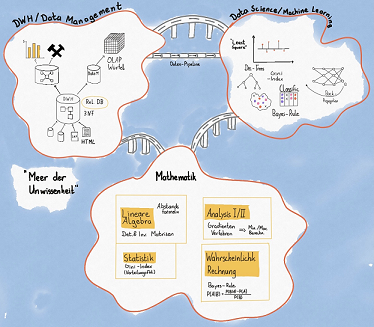
\includegraphics{DWH-Zeichnung}\\
   \small "3-Insel-Bild"  
   %\includegraphics{dhbw_logo} 
   %\begin{figure}
   %\epsfig{file=DHBW-Logo-BW.pdf, scale=0.1}
   %\end{figure}
       
   \vfill
   \large   
   
   Dr. Hermann Völlinger, Mathematik und IT Architektur
           \\ Stuttgart, Herbst 2024     

   \vspace{0.6cm}
        
   \end{center}
   
\begin{center}
Diese Version V0.78 (Datum: 20.07.2024) ist nicht final!!! \\
{\color{red}{(Beachte: ************ Kommentare *********)}} \\[0.3cm]
Aktuelle Versionen findet man in meinem GitHub\\[0.1cm]
\url{https://github.com/HVoellinger/Mathematische-Grundlagen_von_ML/blob/main/Math+MaschLernen(ML)v0.78.pdf} \\
\vspace{0.4cm}
\begin{large}
Dieses Skript wurde generiert mit \LaTeX\  
\end{large}
\end{center}

%\includegraphics[width=0.4\textwidth]{dhbw.gif}
% Department Name\\ Fakultät Technik-Informatik
  
\end{titlepage}

\begin{LARGE} Inhaltsangabe \end{LARGE}

\tableofcontents

\newpage

\begin{LARGE} Bilderverzeichnis \end{LARGE}

\listoffigures 

\newpage

\begin{LARGE} Tabellenverzeichnis \end{LARGE}

\listoftables 

\newpage

\pagenumbering{arabic} % arabische Seitennummerierung für den Hauptteil
 
\renewcommand{\labelenumi}{(\alph{enumi})}
\renewcommand{\labelenumii}{\arabic{enumii}.}

\fancyfoot[C]{--- \thepage/\pageref{LastPage}\ ---}

\section{Management Zusammenfassung - Motivation und Ziele}

Ziel der Ausarbeitung ist es, die {\color{blue}mathematischen Konzepte des Maschinellen Lernens (ML)} zu erkennen.

\subsection{Meine Motivation und Ziele der Arbeit}
Die Anregung zur Erstellung dieses Skriptes liegen in den Erfahrungen, die ich bei meinen DHBW Vorlesungen in Stuttgart zur "Einführung in das Maschinelle Lernen (ML)" festgestellt habe. Viele Studenten habe große Probleme, mathematische Aussagen zu Verstehen und deren Bedeutung für ML zu begreifen.
\\
Dies führte in einigen Fällen auch zum Abbruch des "Data Science" Studienganges. Meine beruflichen Erfahrungen im Bereich der Projektberatung für Data Warehouse Projekte bestätigen dies.\\
Leider wird in der gängigen Literatur dieses Thema nicht genug gewürdigt. Dies mag damit zu tun haben, das heutzutage mathematische Ausbildung in der Schule und in der Universität etwas den Bezug zur Realität verloren hat, und deshalb viele Schüler und Studenten den Nutzen und die Schönheit der Mathematik nicht erkennen können. Es gehört ja manchmal schon "zum guten Ton", wenn technische Hochschulabsolventen fast schon scherzhaft sagen, dass Sie mit Mathematik "nichts am Hut haben".\\
Dies ist leider sehr schade und ist zudem beim Lösen von ML Fragestellungen eine große Hürde. Viele Studenten im "Data Science" Bereich scheitern deshalb auch an mangelnden Mathematik Kenntnissen.\\[0.2cm]
%
Das Ziel der Ausarbeitung ist es deshalb zu zeigen wie nützlich mathematische Ideen bei der Lösung der Fragestellungen des Maschinellen Lernens (aka: \url{https://en.wikipedia.org/wiki/Machine_learning}) sind.\\
Hierfür werden wir mit vielen anschaulichen, aber nicht trivialen Beispielen starten, mit deren Hilfe wir die Arbeitsweise des mathematischen Verfahrens leichter erkennen können. Die Studenten können die prinzipiellen Arbeitsweisen und Methoden der Algorithmen somit erkennen. Die Studenten werden zudem durch geeignete Übungsbeispiele angeregt die Beispiele zu Verallgemeinern. Zu jedem Kapitel gibt es Übungen, die das im Kapitel Gelernte nochmals an konkreten Fragestellungen und Problemen erproben und vertiefen. \\
Musterlösungen bzw. Hinweise zur Lösung der Übungen findet man am Ende des Skriptes. Die Umsetzung dieser Beispiele in allgemeine mathematische Aussagen unter Nutzung des mathematischen Kalküls wird damit leichter und verständlicher vorbereitet (nach dem Prinzip: „Vom Speziellen zum Allgemeinen“). \\[0.2cm]\\
Es werden zudem zahlreiche Hinweise auf vertiefende Anwendungen oder Informationen durch Internet-Links oder weiterführende Literatur gegeben. An vielen Stellen werden konkrete Umsetzungsbeispiele mit Werkzeugen wie \textit{KNIME Analytics Platform} gezeigt. \\
Die Umsetzung dieser Beispiele in allgemeine mathematische Aussagen unter  Nutzung des mathematischen Kalküls wird damit leichter und verständlicher vorbereitet.\\[0.2cm]
%
Die Beziehungen ("Brücken") zwischen Mathematik, Maschinellen Lernen (ML) und Data Science (DL) (insbesondere \href{https://en.wikipedia.org/wiki/Data_mining}{Data Mining} werden konkret gebaut und anschließend beispielhaft "beschritten" (siehe auch "3-Insel-Bild" von der Titelseite).\\\\[0.3cm] 
%
Die Leser sollen befähigt werden, die Mathematik hinter den ML Anwendungen zu verstehen um mögliche weitere sinnvolle Ergänzungen und Erweiterungen, die sich aus den mathematischen Erkenntnissen ergeben, zu entwickeln.\\

\subsection{Brücke "DWH nach ML"im "3-Insel-Titelbild"}
Das Ziel dieses Papiers liegt in einer Vertiefung des Verständnisses der Brücke zwischen Mathematik und ML. Diese Brücke wird auch in den folgenden Kapiteln ausführlich beschrieben. Ein weiterer wichtiger Input für das Verständnis von ML liegt jedoch auch in der Brücke zwischen Data-Management/DWH und ML. Zu diesem Thema werde ich im folgenden Unterkapitel einige wichtige Anmerkungen und Aussagen machen.\\[0.1cm]
Über diese Brücke fließen nicht nur Daten sondern auch Metadaten. Metadaten sind für das Verständnis eines DWH sehr wichtig. Siehe auch dazu die Vorlesung zu Thema DWH [HVö-LecDWH23].\\
Diese Metadaten spielen jedoch auch ein wichtige Rolle bei der Entwicklung von ML Algorithmen und Modellen. Insbesondere wenn wir hier an das Thema vom Aufbau grosser Sprachmodelle (aka LLM) denken. Siehe hierzu auch das Kapitel im Anhang über LLM's (i.e. ChatGPT). \\[0.2cm] 
%
Wo stecken also diese Metadaten im DWH? Hier möchte ich beispielhaft zwei Werkzeuge erwähnen und zwar die Werkzeuge zur Datenmodellierung (z.B. Infosphere Data Architect -IDA) und Data Governance (z.B. Infosphere Governance Catalog - IGC). Beide Werzeuge wurden ausführlich in der DWH Vorlesung (siehe [HVö-LecDWH23], Seite 25 und Seiten 130-132) besprochen. \\[0.1cm] 
\subsubsection{Details zu IDA und IGC}
\textbf{IDA:} IBM InfoSphere Data Architect ist eine kollaborative Lösung für die Modellierung und das Design von Unternehmensdaten, die das Integrationsdesign für Business Intelligence-, Master Data Management- und Service-orientierte Architekturinitiativen vereinfacht und beschleunigt. IDA ermöglicht die Zusammenarbeit mit Anwendern in jedem Schritt des Datendesignprozesses, vom Projektmanagement über das Anwendungsdesign bis hin zum Datendesign. Das Tool hilft dabei, Prozesse, Dienste, Anwendungen und Datenarchitekturen aufeinander abzustimmen. Sehen Sie in [DHBW-Moodle] das Video: 'Demo-Infosphere Data Architect (IDA).mp4' .\\[0.2cm]
%
\begin{figure}[htp]
  \centering
  \hspace*{-0.1cm} 
  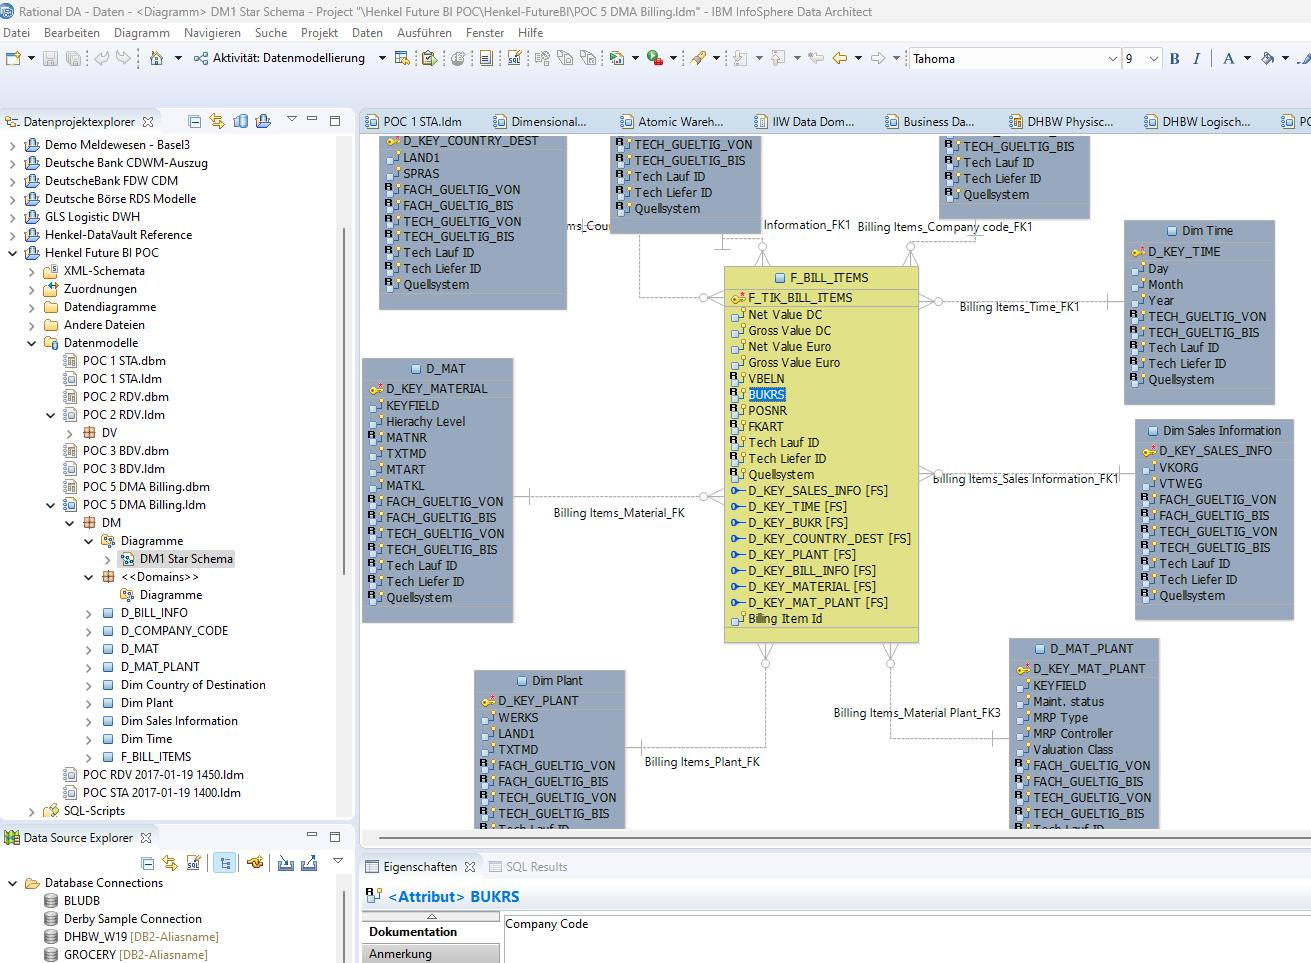
\includegraphics[width=0.9\textwidth]{IDA-Datamart}
  \caption{Beispiel für ein Datamart Modell unter IDA}
  \label{fig:IDA-Datamart}
\end{figure}
\\[4.2cm] 
%
\textbf{IGC:} IBM InfoSphere Information Governance Catalog (IGC) ist ein interaktives, webbasiertes Tool, mit dem Benutzer ein Unternehmensvokabular und ein Klassifizierungssystem in einem zentralen Katalog erstellen, verwalten und gemeinsam nutzen können. Es hilft den Anwendern, die geschäftliche Bedeutung ihrer Assets zu verstehen und bietet Such-, Browse- und Abfragefunktionen. Darüber hinaus können die Benutzer Asset-Sammlungen erstellen und Berichte über den Datenfluss zwischen Assets erstellen. Siehe in [DHBW-Moodle] die folgenden Dokumente und Videos:
'Geführte IGC Demo.pdf'; Geführte IGC Demo - Deutsch.pdf'; 'Demo-IGC-Teil1.mp4'; 'Demo-IGC-Teil2.mp4' und 'Demo Qutput-IGC-Teil2-Data Lineage.pdf'. \\[0.2cm] 
%
\begin{figure}[htp]
  \centering
  \hspace*{-0.1cm} 
  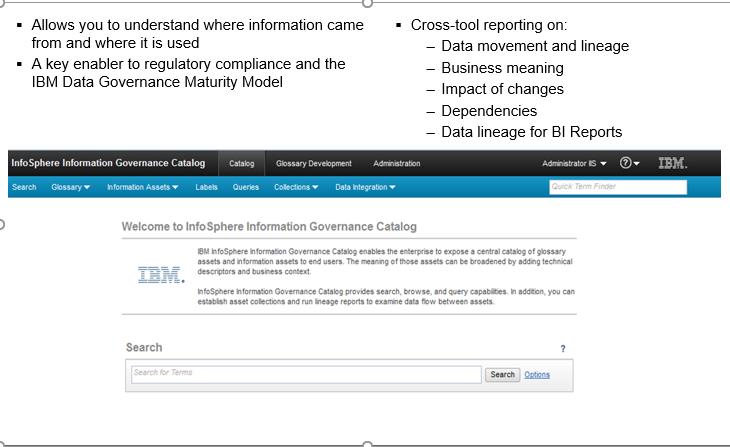
\includegraphics[width=0.95\textwidth]{IGC-Overview}
  \caption{Einstiegsmaske in IGC}
  \label{fig:IGC-Overview}
\end{figure}
%
\\[0.2cm] 
%
\subsubsection{Nutzen der IDA und IGC Strukturen für ML}
%
Im nächsten Beispiel sehen wir wie Technische Assets (z.B. Spaltennamen einer Tabelle) mit fachlichen Begriffen ("Business Terms") verbunden werden. Dadurch erhalten wir eine fachliche Beschreibung und Kategorisierung/Strukturierung) der fachlichen Asssts im DWH.\\[0.2cm] 
%
\begin{figure}[htp]
  \centering
  \hspace*{-0.1cm} 
  \includegraphics[width=0.95\textwidth]{Business Term mit zugehörigen technischen Assets}
  \caption{Business Term mit zugehörige Assets}
  \label{fig:IGC-BT+TA}
\end{figure}
\\[0.2cm]
Im obigen Beispiel sehen wir den Geschäftsbegriff „Buchungskreis“, zu dem das Feld mit dem Namen „BUKRS“ in 7 Tabellen in verschiedenen Datenschichten des DWH gehört. 
Diese Information erklärt die betriebswirtschaftliche Bedeutung dieses Feldes und gibt auch an, wo dieses Feld im DWH vorkommt. Dies ist sowohl für die Analyse/Auswertung der Daten als auch für den Datenpopulationsprozess (ETL) beim Laden der Daten in das DWH von entscheidender Bedeutung. Zudem ist diese Strukturierung bei Bau eines LLM Modells in ML sehr hilfreich.\\
Eine weitere nützliche Info ist die sogenannte "Data Lineage", die den kompletten Verarbeitungsprozess (inklusive und Datenablagen) im DWH abbildet. Die zugehörige Business Lineage ze.gt nur die Datenablage ohne die ETL Prozesse dazwischen darzustellen. Zusammengefasst: \\
Data Lineage: Technisch orientiert, detaillierte Nachverfolgbarkeit der Datenflüsse und Transformationen innerhalb der IT-Infrastruktur.\\
Business Lineage: Geschäftlich orientiert, höher abstrahierte Darstellung der Datenflüsse und Nutzung in Geschäftsprozessen und -anwendungen.\\
Beide Konzepte sind wichtig für eine umfassende Daten-Governance-Strategie. Data Lineage bietet die technische Grundlage, während Business Lineage das Verständnis und die Transparenz aus der Geschäftsperspektive fördert. 
\\[0.5cm] 
%
\begin{figure}[htp]
  \centering
  \hspace*{-0.1cm} 
  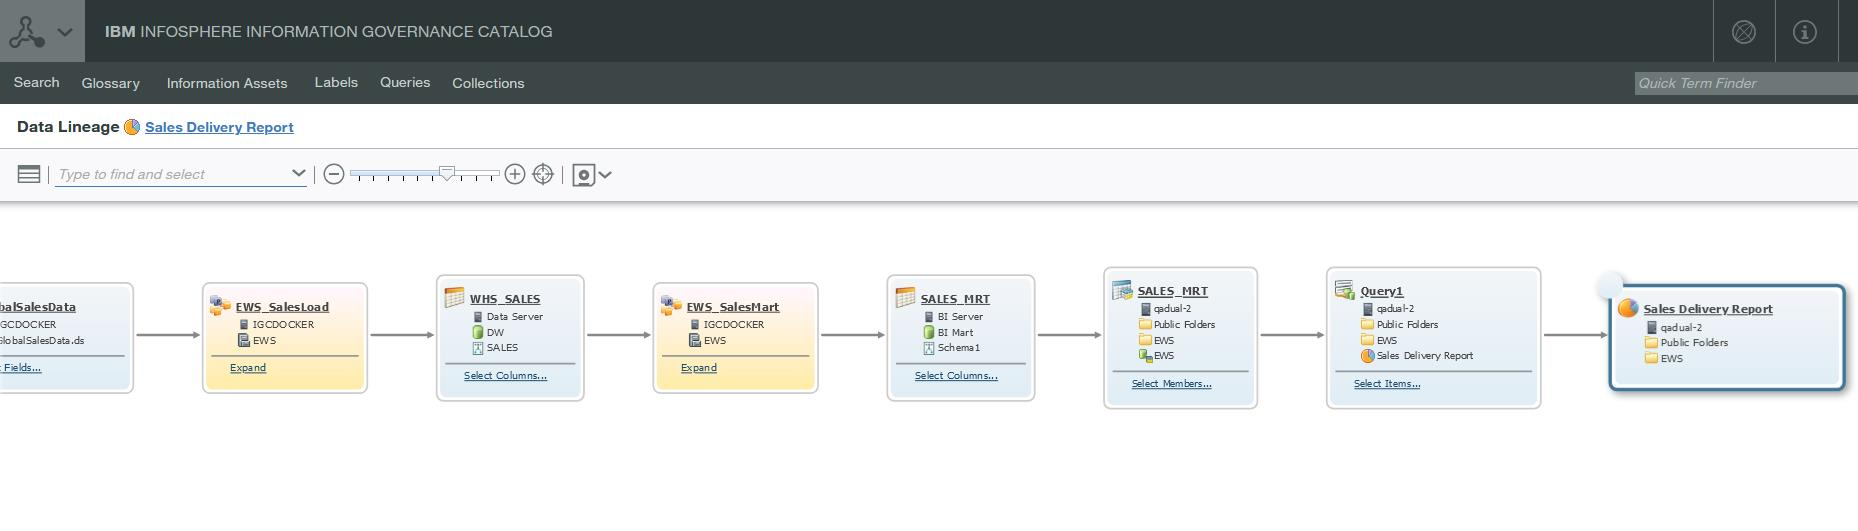
\includegraphics[width=0.95\textwidth]{IGC-DataLineage}
  \caption{Data Lineage für einen BI Report in IGC}
  \label{fig:IGC-DataLineage}
\end{figure}\\[0.2cm]
\textbf{Zusammenfassung - Nutzen für ein LLM:}\\[0.2cm]
Zusammengefasst ist Data Governance beim Aufbau eines LLMs von zentraler Bedeutung, um sicherzustellen, dass die Datenqualität hoch ist, Bias minimiert wird, Datenschutz und -sicherheit gewährleistet sind, Transparenz und Verantwortlichkeit gefördert werden und letztlich ein leistungsfähiges, genaues und vertrauenswürdiges Modell entsteht. \\[0.1cm]
Weiterführende bzw. vertiefende Literatur zu diesem Thema findet man unter den Referenzen \textbf{[TDWI-Feature Learning]} oder unter \textbf{[TDWI-Datenflüsse]}       \\[0.2cm]
%
\subsection{Überblick über die Mathematischen Methoden}
Die mathematischen Grundlagen des Maschinellen Lernens ("Machine Learning") umfassen mehrere Bereiche der Mathematik, die für das Verständnis und die Entwicklung von Machine Learning Algorithmen von Bedeutung sind.
Hier sind die wichtigsten \textbf{mathematische Konzepte und Grundlagen:}\\[0.3cm]
%
\textbf{1. Lineare Algebra:} Lineare Algebra ist ein grundlegender Bestandteil des Maschinellen Lernens "Machine Learning". Vektoren und Matrizen werden verwendet, um Daten darzustellen, und Operationen wie Skalierung, Addition, Multiplikation und Transformationen werden angewendet, um Berechnungen durchzuführen. Matrixoperationen wie Matrixmultiplikation und Matrixinversion sind wichtig für viele Algorithmen.\\[0.2cm]
%
\textbf{2. Differentialrechnung:} Differentialrechnung wird verwendet, um Funktionen zu analysieren und Optimierungsalgorithmen abzuleiten. Berechnung von Gradienten, Ableitungen, partielle Ableitungen und Optimierungsmethoden wie das Verfahren zum Gradientenabstieg sind entscheidend für das Trainieren von Modellen und das Anpassen von Parametern.\\[0.2cm]
%
\textbf{3. Wahrscheinlichkeitstheorie und Statistik:} Wahrscheinlichkeitstheorie und Statistik spielen eine wichtige Rolle im Machine Learning, insbesondere im Bereich des überwachten und nicht überwachten Lernens. Wahrscheinlichkeitsverteilungen, Schätzungen, Hypothesenbildung und statistische Modelle werden verwendet, um Muster in den Daten zu erkennen, Vorhersagen zu treffen und Unsicherheiten zu quantifizieren.\\[0.2cm]
%
\textbf{4. Optimierung:} Optimierungsmethoden werden verwendet, um Modelle zu trainieren und die besten Parameterwerte zu finden. Die Optimierungstechniken umfassen lineare Programmierung, konvexe Optimierung und nichtlineare Optimierung.\\[0.2cm]
%
\textbf{5. Informationstheorie:} Informationstheorie befasst sich mit der Quantifizierung und Übertragung von Informationen. Konzepte wie Entropie, Informationsgewinn und Kompressionsalgorithmen spielen eine Rolle in der Modellierung und Auswahl von Merkmalen sowie in der Reduzierung der Komplexität von Daten.\\[0.2cm]
%
Diese mathematischen Grundlagen werden verwendet, um Modelle zu definieren, Daten zu analysieren, Funktionen anzupassen, Vorhersagen zu treffen und Modelle zu evaluieren. Sie dienen als Grundlage für das Verständnis der Algorithmen und Methoden des Machine Learning. Es ist wichtig, ein solides Verständnis dieser mathematischen Konzepte zu haben, um Machine Learning effektiv anzuwenden und weiterzuentwickeln.
%
\subsection{Historische Anmerkungen zu Mathematik und ML}
%
Vor etwa 250 Jahren begann man, die Mathematik zu formalisieren, aber erst vor etwa 100 Jahren wurde die moderne Mathematik entwickelt. Es handelt sich um ein riesiges Fachgebiet, mit vielen Unterbereichen, wie Lineare Algebra, Statistik, etc. sowie mit Anwendungen in den Ingenieurwissenschaften und der Physik.\\[0.2cm]
Die Nutzung von Mathematik in Machine Learning ist eine grundlegende Komponente der Entwicklung von Algorithmen und Modellen. Hier sind einige historische Anmerkungen zur Verwendung von Mathematik in diesem Bereich:\\[0.2cm]
\textbf{1. Entwicklung der linearen Regression (19. Jahrhundert):} \\
Die lineare Regression ist ein grundlegendes statistisches Modell, das in Machine Learning weit verbreitet ist. Es wurde im 19. Jahrhundert entwickelt und nutzt mathematische Konzepte wie die Methode der kleinsten Quadrate, um Beziehungen zwischen Variablen zu modellieren.\\[0.2cm]
\textbf{2. Perzeptron (1957)}\\
Der Perzeptron-Algorithmus, entwickelt von Frank Rosenblatt, war einer der frühen Versuche, maschinelles Lernen formal mathematisch zu modellieren. Es basierte auf der Idee von künstlichen Neuronen und wurde für die Klassifikation verwendet.\\[0.2cm]
\textbf{3. Gradientenabstiegsverfahren (1960er Jahre):} \\
Das Gradientenabstiegsverfahren ist ein wichtiger Optimierungsalgorithmus in der Mathematik, der später in vielen Machine-Learning-Verfahren wie Neuronalen Netzen, Support Vector Machines und tiefen Lernalgorithmen verwendet wurde.\\[0.2cm]
\textbf{4. Bayes'sche Statistik (18. Jahrhundert):}\\
Die Bayes'sche Statistik und das Bayes'sche Theorem, das auf dem Werk von Thomas Bayes basiert, sind grundlegende mathematische Konzepte, die in probabilistischen Machine-Learning-Modellen wie dem Naive Bayes-Klassifikator Anwendung finden.\\[0.2cm]
\textbf{5. Entwicklung von neuronalen Netzen (1940er Jahre - heute):}\\
Neuronale Netze, die in vielen modernen Machine-Learning-Anwendungen eine zentrale Rolle spielen, basieren auf mathematischen Modellen von künstlichen Neuronen und sind eng mit der Linearen Algebra und dem Konzept der Backpropagation verbunden.\\[0.2cm]
\textbf{6. Entwicklung von tiefen neuronalen Netzen (2010er Jahre):}\\
Die jüngste Entwicklung von tiefen neuronalen Netzen, die in Deep Learning eingesetzt werden, beruht auf fortgeschrittenen mathematischen Konzepten, insbesondere der Backpropagation, die es ermöglichen, komplexe Modelle zu trainieren.\\[0.3cm]
%
Die Verwendung von Mathematik in Machine Learning ist also keine neue Entwicklung, sondern hat eine lange Geschichte. Mit der Zeit wurden jedoch immer leistungsfähigere mathematische Techniken entwickelt und angewendet, um komplexe Modelle zu erstellen und große Datenmengen zu verarbeiten. Diese Entwicklung setzt sich fort, da Machine Learning und künstliche Intelligenz weiterhin stark erforscht und weiterentwickelt werden.
\\[0.2cm]
%
\newpage
%
\section{Wichtige Anwendungen der Mathematik in ML}

In diesem Skript/Buch werden Sie unter anderen sechs konkrete Beispiele für Mathematik bei bekannten Verfahren des Maschinellen Lernen (ML) kennenlernen. Pro Verfahren gibt es ein separates Kapitel im Skript.\\
Die einzelne Kapitel werden durch anschauliche Beispiele motiviert und  ergänzt. Anhand dieser Beispiele kann mal auch schnell und anschaulich die allgemeinen mathematischen Grundlage der entsprechenden ML Verfahren nachvollziehen.\\
Zu den einzelnen Kapitel Themen gibt es jeweils mehrere Übungen bzw. Hinweise zu deren Lösung.\\
Diese sechs ML Verfahren sind:\\

%\begin{enumerate}
%\item[\color{blue}{1. text}]
%\item \blue{\item[2. text]
%\item[3. text]
%\end{enumerate}

1. Mathematik zum k-Means-Algorithmus ("Euklidische Geometrie")\\

2. Entscheidungsbäume mit GINI-Index und ID3-Verfahren (Statistik)\\

3. Lineare Regression und "Best Fit" Verfahren der Analysis (AN)\\

4. Text-Klassifikation mit Bayes-Verfahren (Bedingte Wahrscheinlichkeiten)\\
 
5. Verfahren der "Support Vector Machines" (SVM) via "Kernel-Trick"\\

6. Neuronale Netzwerke und Backpropagation via "Absteigende Gradienten"\\[0.2cm]
%
Am Ende kommt noch ein Kapitel \textbf{Anhang} in den sechs weitere ML-Verfahren der Vollständigkeit halber eher kurz erläutert werden. Diese sind:\\

1. Empfehlungssysteme "Recommender Systems" (LinAlgebra)\\

2. Regularisierungen "Regularization" und Lin. Algebra (LA)\\

3. Hauptkomponenten-Analyse "Principal Component Analysis" (PCA)\\
 
4. Singulärwertzerlegung "Singular Value Decomposition" (SVD)\\
 
5. Mathematische Verfahren im NLP, i.e. "Latent Semantic Analysis/Indexing (LSI)"?\\

6. Mathematik und grosse Sprachmodelle "Large Language Models" (LLMs))

\newpage

\section{Mathematik zum "k-Means-Algorithmus" \\}

Ein {\color{blue}{k-Means-Algorithmus}}\index{k-Means-Algorithmus} ist ein Verfahren der Euklidischen Geometrie. Dabei wird aus einer Menge von ähnlichen Objekten eine vorher bekannte Anzahl von k Gruppen ("Clustern") gebildet.\\
Der Algorithmus ist eine der am häufigsten verwendeten Techniken zur Gruppierung von Objekten, da er schnell die Zentren der Cluster findet. Dabei bevorzugt der Algorithmus Gruppen mit geringer Varianz und ähnlicher Größe.\\
Der Algorithmus hat starke Ähnlichkeiten mit dem "Erwartungs-Maximierungs-Algorithmus (EM-Algorithmus)" und zeichnet sich durch seine Einfachheit aus.\\
Erweiterungen sind der $"k-Median-Algorithmus"$ und der $"k-Means++ Algorithmus" $.\\

\subsection{Problemstellung und Mathematik}

Ziel von k-Means ist es einen den Datensatz so in $k$ Partitionen zu teilen, dass die Summe der quadrierten Abweichungen von den Cluster-Schwerpunkten minimal ist. Mathematisch entspricht dies der Optimierung der Funktion F:\\
\begin{center}
$ F = \sum_{i=1}^{k}  \sum_{\mathbf x_j \in S_{i}} {\| \mathbf x_j - \boldsymbol \mu_i \|^2}$ \\[0.2cm]
mit den Datenpunkten $ \mathbf x_j $ und \\
den "Schwerpunkten" $ \boldsymbol \mu_i $ der Cluster $ S_i $.\\[0.2cm]
\end{center}
%
Diese Zielfunktion basiert auf der \textbf{Methode der kleinsten Quadrate} und man spricht auch von "Clustering durch Varianzminimierung", da die Summe der Varianzen der Cluster minimiert wird.\\[0.2cm]
Da zudem $ \| \mathbf x_j - \boldsymbol \mu_i \|^2 $ die quadrierte "Euklidische Distanz" ist, ordnet k-Means effektiv jedes Objekt dem nächstgelegenen (nach Euklidischer Distanz) Clusterschwerpunkt zu.\\ 
Eine Visualisierung der k-Means-Konvergenz Iterationen, sehen wir im der folgenden Figur.
\newpage
%
\begin{figure}[htp]
  \centering
  \hspace*{-0.1cm} 
  \includegraphics[width=0.7\textwidth]{k-Means-Konvergenz-Iteration0}
  \caption{k-Means-Konvergenz-Iterationen(0-14)}
  \label{fig:k-Means-Iteration0}
\end{figure}
%
Um eine Animation dieser 3-Means-Konvergenz mit insgesamt 15 Iterationen zu sehen können sie auch folgenden Link auf mein GitHub aufrufen:\\
\url{https://github.com/HVoellinger/Mathematische-Grundlagen_von_ML/blob/main/Images/k-Means-Konvergenz-Animation.gif}\\

\subsection{k-Means Algorithmen}

Da die Suche nach der optimalen Lösung schwer ist, wird im Normalfall ein approximativer Algorithmus verwendet wie die \textbf{ Heuristiken von Lloyd oder MacQueen}. Da die Problemstellung von k abhängig ist, muss dieser Parameter vom Benutzer festgelegt werden.\\

\subsubsection{Lloyd-Algorithmus}

Der am häufigsten verwendete {\color{blue}{k-Means-Algorithmus}} \index{k-Means-Algorithmus} ist der \textbf{Lloyd-Algorithmus}, der oft als "der k-Means-Algorithmus" bezeichnet wird, obwohl Lloyd diesen Namen nicht verwendet hat. Lloyds Algorithmus besteht aus drei Schritten:\\[0.2cm]
\textbf{1. Initialisierung:} Wähle $k$ zufällige Mittelwerte ("Means"): $ \mathbf m_1^{(1)}, \ldots, \mathbf m_k^{(1)} $ aus dem Datensatz.\\
\textbf{2. Zuordnung:} Jedes Datenobjekt wird demjenigen Cluster zugeordnet, bei dem die Cluster-Varianz am wenigsten erhöht wird.
\begin{center}
$ S_i^{(t)} = \left\{ \mathbf x_j : \big\| \mathbf x_j - \mathbf m^{(t)}_i \big\|^2 \leq \big\| \mathbf x_j - \mathbf m^{(t)}_{i^*} \big\|^2 \text{ für alle }i^*=1,\ldots,k \right\}$\\[0.2cm]
\end{center}
\textbf{3. Aktualisieren:} Berechne die Mittelpunkte der Cluster neu.
\begin{center}
$ \mathbf m_i^{(t+1)} = \frac{1}{|S_i^{(t)}|} \sum_{\mathbf x_j \in S_{i}^{(t)}} \mathbf x_j  $ \\
\end{center}
Die Schritte 2–3 werden dabei so lange wiederholt, bis sich die Zuordnungen nicht mehr ändern.

\subsubsection{MacQueen'sLloyd-Algorithmus} 

MacQueen führte mit dem Begriff k-Means einen anderen Algorithmus ein:
\\[0.3cm]1. Wähle die ersten $k$ Elemente als Clusterzentren.\\
2. Weise jedes neue Element dem Cluster zu, bei dem sich die Varianz am wenigsten erhöht, und aktualisiere das Clusterzentrum.
\\[0.3cm]Während es ursprünglich – vermutlich – nicht vorgesehen war, kann man auch diesen Algorithmus iterieren, um ein besseres Ergebnis zu erhalten.

\subsection{Python Programm zum k-Means-Clustering}

{\color{red}{***********************************************************************\\ 
Ab hier bis Ende der Section sind die Folien der Vorlesung ML  zu nutzen und diese sind in Latex umzusetzen...\\
************************************************************************}}\\[0.2cm]


\begin{center}
\hspace*{-2.0cm}   
\includegraphics[width=1.0\textwidth]{K-Means-Python-Bild1}
\hspace*{-2.0cm}   
\includegraphics[width=1.0\textwidth]{K-Means-Python-Bild2}
\hspace*{-2.0cm} 
\includegraphics[width=1.0\textwidth]{K-Means-Python-Bild3}
\hspace*{-2.0cm} 
\includegraphics[width=1.0\textwidth]{K-Means-Python-Bild4}
\end{center}

\subsection{k-Means-Clustering für IRIS Blumen}


Der in diesem Beispiel verwendete Datensatz ist der berühmte {\color{blue}{IRIS-Blumen Datensatz}} \index{IRIS-Blumen Datensatz} Er besteht aus 150 Einträgen der Irisblume, die jeweils durch vier Merkmale beschrieben werden: Kelchblattlänge, Kelchblattbreite, Blütenblattlänge und
Blütenblattbreite. \\[0.2cm]
Zusätzlich ist der spezifische Typ der Irisblume angegeben. Es gibt drei Arten
der Schwertlilienpflanze: Iris Setosa, Iris Versicolor und Iris Virginica.\\
Jede Art ist mit mit 50 Einträgen im Datensatz vertreten. Die Merkmale sind in Zentimetern angegeben. Die Abbildung unten zeigt wie die Daten im Datenrahmen dargestellt werden. Der Datensatz wurde erstmals von Ronald Fisher, einem britischen Biologen, in einem Aufsatz aus dem Jahr 1936 vorgestellt. Er ist eines der am häufigsten verwendeten Beispiele für statistischen Klassifizierung-Algorithmen beim Maschinellen Lernen. \\
Die Abbildung unten zeigt die ersten fünf Einträge des Datensatzes. Der Datensatz ist in der Python-Bibliothek scikit-learn enthalten.\\ 

\begin{figure}[htp]
  \centering
  \hspace*{-0.1cm} 
  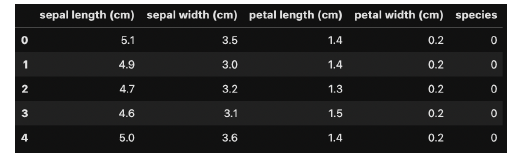
\includegraphics[width=0.9\textwidth]{IRIS-Dataset-First_Entries}\\
  \caption{Die ersten 5 Entries im IRIS Datensatz}
  \label{fig:Iris_DS}
\end{figure}
%
Siehe Lösungen in meinem Github:\\ 
%
\url{https://github.com/HVoellinger/Mathematische-Grundlagen_von_ML/blob/main/Quellen_Math-ML/k-means-HVoe.pdf} \\
%
\url{https://github.com/HVoellinger/Mathematische-Grundlagen_von_ML/blob/main/Quellen_Math-ML/k-means-HVoe.tex}\\[0.3cm]
%
Die Konfusion-Matrix zeigt, dass alle 50 setosa-Blüten richtig klassifiziert wurden.\\ 48 versicolor-Blüten wurden richtig klassifiziert, aber 14 wurden falsch erkannt. \\ 36 virginica-Blüten wurden richtig beschriftet und 2 virginica-Blüten wurden fälschlicherweise als virginica-Blüten klassifiziert.\\[0.2cm]
%
Insgesamt funktionieren  Clustering und Klassifizierung mit k-Means im {\color{blue}{IRIS-Blumen Datensatz}} \index{IRIS-Blumen Datensatz} gut. Mit einer Genauigkeit von 89 Prozent ist der Algorithmus ein gutes Hilfsmittel, um ein Modell für die Vorhersage der genauen Art der Irisblüte zu erstellen.\\
Wie die Konfusion-Matrix zeigt, ist die Klassifikation zu 100\% genau
für die Setosa-Blüten und über 94\% für die Versicolor-Arten. Es scheitert nur bei der genauen Virginica-Blüten mit einer Genauigkeit von "nur" 77\%.\\
Das Modell von k-Means kann jedoch noch weiter verbessert werden, wie andere  Implementierungen wie k-means++ zeigen. Es verbessert außerdem die Wahl der anfänglichen Zentren.

\newpage

{\color{red}{***********************************************************************\\ 
Ab hier bis Ende der Übungen sind die Folien der Vorlesung ML  zu nutzen und diese sind in Latex umzusetzen...\\
************************************************************************}}\\[0.2cm]
\subsection{Übungen zum Kapitel 3}
.....\\
\subsubsection{Übung 3.1 - nnn1}
TEXT\\
\subsubsection{Übung 3.2 - nnn2}
.....\\
\subsubsection{Übung 3.3 - ...............}


\newpage

\section{Lernen von Entscheidungsbäumen ("Decision Tree")\\}


\textbf{Entscheidungsbaum-Algorithmen} sind weit verbreitete Methoden im maschinellen Lernen, die zur \textbf{Klassifikation und Regression} verwendet werden.\\

\subsection{Mathematik bei Entscheidungsbäumen}

Es gibt verschiedene mathematische Verfahren und Techniken, die bei der Konstruktion und Optimierung von Entscheidungsbäumen eingesetzt werden. Hier sind einige davon:\\[0.2cm]
%
\textbf{1. Entropie und Informationsgewinn:}\\
Die Entropie ist ein Maß für die Unordnung oder Unsicherheit in einem Datensatz. Beim Konstruieren eines Entscheidungsbaums wird der Informationsgewinn verwendet, um festzustellen, wie gut eine Funktion (Attribut) den Datensatz in Bezug auf die Zielvariable aufteilt. Der Informationsgewinn wird oft in Form von Entropieänderungen zwischen den ursprünglichen und den aufgeteilten Datensätzen gemessen.\\[0.2cm]
%
\textbf{2. Gini-Index}\\
Der Gini-Index misst die Wahrscheinlichkeit, dass eine zufällig ausgewählte Instanz falsch klassifiziert wird, wenn sie zufällig nach den Klassenverteilungen in einem Teilbaum ausgewählt wird. Ein niedriger Gini-Index deutet auf eine homogene Verteilung der Klassen hin.\\[0.2cm]
%
\textbf{3. Reduktion des quadratischen Fehlers (Regression):}\\
Bei Entscheidungsbäumen für Regression werden mathematische Kriterien wie die Reduktion des quadratischen Fehlers verwendet, um die besten Aufteilungen der Daten zu finden, die zu einer geringeren Varianz der Zielvariablen führen.\\[0.2cm]
%
\textbf{4. Cost-Complexity-Pruning:}\\
Nach dem Konstruieren eines Entscheidungsbaums können zu viele Verzweigungen zu Overfitting führen. Das Cost-Complexity-Pruning verwendet eine Kostenfunktion, um die Qualität eines Baums in Bezug auf seine Komplexität zu bewerten. Durch Entfernen von Verzweigungen, die nur geringfügig zur Verbesserung der Modellgenauigkeit beitragen, kann die Generalisierungsfähigkeit des Baums verbessert werden.\\[0.2cm]
%
\textbf{5. CART (Classification and Regression Trees):}\\
Der CART-Algorithmus verwendet eine rekursive Zweig- und Bindemethode, um einen Baum zu erstellen. Er sucht nach der besten Spaltung eines Datensatzes anhand des Gini-Index (für Klassifikation) oder der Reduzierung des quadratischen Fehlers (für Regression).\\[0.2cm]
%
\textbf{6. Random Forests und Boosting:}\\
Diese Ansätze basieren auf Entscheidungsbäumen, werden jedoch durch die Kombination mehrerer Bäume oder das Hinzufügen von Gewichten zu den Instanzen verbessert. Sie nutzen mathematische Methoden, um die Vorhersagegenauigkeit und Robustheit zu erhöhen.\\[0.2cm]
%
\textbf{6. Hyperparameter-Optimierung:}\\
Die Wahl der Hyperparameter, wie beispielsweise die maximale Tiefe des Baums oder die Mindestanzahl der Instanzen in einem Blatt, beeinflusst die Leistung des Entscheidungsbaums. Mathematische Verfahren wie Rastersuche oder Bayes'sche Optimierung können verwendet werden, um die besten Hyperparameter für das Modell zu finden.\\[0.2cm]
%
\textbf{Zusammenfassung}:
Diese Verfahren sind alle Teil des Prozesses der Konstruktion, Anpassung und Optimierung von Entscheidungsbäumen im maschinellen Lernen. Die Wahl des geeigneten Verfahrens hängt von der Art des Problems und den Daten ab, mit denen Sie arbeiten.\\[0.4cm]

\subsection{Mathematische Grundlagen Gini-Index und Entropie-Verfahren}


\subsubsection{Gini-Index Verfahren}
%
Das {\color{blue}{Gini-Index Verfahren}}\index{Gini-Index Verfahren} ist eine Technik zur Aufteilung von Entscheidungsbäumen, insbesondere im Kontext von Klassifikationsproblemen. Der Gini-Index misst die Unreinheit oder den Mischungsgrad der Daten an einem bestimmten Punkt im Baum.\\
Er wird oft für die Auswahl von Splits in einem Entscheidungsbaum verwendet. \\
Der "klassische" Gini-Index für zwei Zielvariablen i und j mit den entsprechenden Wahrscheinlichkeiten $p_i$ und $p_j$ wird durch die folgende Formel dargestellt:
\[
Gini = \sum_{i \neq j} (p_i)\cdot(p_j)
\]
%
Betrachtet man den Fall mit binären Zielvariablen (YES=1 oder NO=0), so gibt es insgesamt vier mögliche Kombinationen der Wahrscheinlichkeiten sodass die Summe 1 ergibt:\\
$P(Target=1)\cdot P(Target=1)+ P(Target=1)\cdot P(Target=0) + P(Target=0)\ \cdot P(Target=1) + P(Target=0) \cdot P(Target=0) = 1.$\\
Also folgt: \\
$P(Target=1).P(Target=0) + P(Target=0)\cdot P(Target=1)= 1 - [P(Target=0)]^2 – [P(Target=1)]^2.$  \\[0.3cm]
Damit wird der Gini-Index für einen bestimmten Knoten durch die folgende Formel dargestellt:
\[
Gini(D) = 1 - \sum_{i=1}^{c} (p_i)^2
\]
%
Hierbei steht \(D\) für den Datensatz im betrachteten Knoten, \(c\) ist die Anzahl der Klassen, und \(p_i\) ist der Anteil der Instanzen der Klasse \(i\) im Knoten.\\[0.2cm]
Der Gini-Index ist eine Zahl zwischen 0 und 1, wobei 0 für einen reinen Knoten (alle Instanzen gehören derselben Klasse an) und 1 für einen maximal unreinen Knoten steht.\\
Wenn ein Entscheidungsbaum trainiert wird, wird der Gini-Index für potenzielle Splits berechnet, und der Split mit dem niedrigsten Gini-Index wird ausgewählt, um den Datensatz zu teilen. Der Prozess wird rekursiv für jeden entstehenden Teilbaum fortgesetzt.\\
Das Gini-Index-Verfahren ist eine beliebte Methode in Entscheidungsbäumen, weil es effizient ist und gut mit kategorialen und numerischen Daten umgehen kann. Es wird oft in Algorithmen wie dem CART (Classification and Regression Trees) verwendet.\\[0.2cm]
\textbf{Beschreibung des Verfahrens an einem einfachen Beispiel:}\\
%
Angenommen, wir haben einen Datensatz mit zwei Klassen (A und B) und zwei Merkmalen (Merkmal 1 und Merkmal 2). Die Zielvariable ist die Klassenzugehörigkeit (A oder B). 
%
\begin{table}[h]
\centering
  \caption{Beispiel zur Knotenberechnung (Gini)}
  \label{tab:Beispiel-Tabelle}
\begin{tabular}{|c|c|c|c|}
\hline
\color{red}{Beispiel} & \color{red}{Merkmal 1} & \color{red}{Merkmal 2} & \color{red}{Klasse} \\
\hline
1 & 2 & 3 & A \\
2 & 1 & 4 & A \\
3 & 3 & 2 & B \\
4 & 4 & 1 & B \\
\hline
\end{tabular}
\end{table}\\[0.3cm]
%
Wir möchten einen Entscheidungsbaum erstellen, um die Klasse vorherzusagen. Beginnen wir mit dem Wurzelknoten. Um den Gini-Index zu berechnen, betrachten wir jede mögliche Aufteilung und wählen diejenige mit dem geringsten Gini-Index.
%
Angenommen, wir betrachten die Aufteilung nach Merkmal 1:
%
\begin{enumerate}
    \item Teilgruppe für (Merkmal 1) $\leq$ 2:
        \begin{itemize}
            \item Beispiele: 1, 2
            \item Gini-Index ( $\leq$ 2): $1 - (1/2)^2 - (1/2)^2 = 0.5$
        \end{itemize}
    \item Teilgruppe für (Merkmal 1) $ > $ 2:
        \begin{itemize}
            \item Beispiele: 3, 4
            \item Gini-Index ($>$ 2): $1 - (1/2)^2 - (1/2)^2 = 0.5$
        \end{itemize}
\end{enumerate}
%
Der gewichtete Durchschnitt der Gini-Indizes beträgt $0.5 \times \frac{2}{4} + 0.5 \times \frac{2}{4} = 0.5$. Das ist der Gini-Index für die Aufteilung nach Merkmal 1.\\[0.2cm]
Wir würden denselben Prozess für Merkmal 2 durchführen und dann die Aufteilung wählen, die den geringsten gewichteten Gini-Index hat.\\
Das ist im Wesentlichen, wie das {\color{blue}{Gini-Index Verfahren}}\index{Gini-Index Verfahren} in einem Entscheidungsbaum angewendet wird.\\[0.4cm]
Wenn man nun allgemein k Merkmale hat, und ein Knoten p in k Partitionen ("Kindknoten") zerlegt ("split") werden könnte, wo wird der Gini-Index des Splits $Gini_{split}$ wie folgt berechnet:

\[
Gini_{split} = \sum_{i=1}^{k} \frac{n_i}{n} \cdot Gini(i)
\]

Hierbei ist:
\begin{align*}
& Gini_{split} \text{{ ist der Gini-Index nach dem Split}}, \\
& Gini(i) \text{{ ist der Gini-Index des Kindknoten i}}, \\
& k \text{{ ist die Anzahl der Kindknoten}}, \\
& n_i \text{{ ist der Anteil der Samples im i-ten Kindknoten.}}\\
& n \text{{ ist der Anteil der Samples im p-ten Knoten.}}
\end{align*}
%
Man wählt als nächsten Knoten dann den Knoten mit dem geringsten $Gini_{split}$.
Für ein besseres Verständnis dieser Formeln und ihrer genauen Anwendung verweisen wir hier auf den nächsten Abschnitt mit konkreten Beispielen und mit konkreten Zahlen.\\
Wenn es sich bei der Zielvariablen um eine kategoriale Variable mit mehreren Ebenen handelt, ist der Gini-Index immer noch ähnlich. Wenn die Zielvariable k verschiedene Werte annimmt, lautet der Gini-Index:
\[
Gini_{kat} = 1 - \sum_{i=1}^{k} p_i^2
\]
%
Der \textbf{minimale} Gini-Index ist = 0, wenn alle Beobachtungen zu einem Label gehören. Der \textbf{maximale} Gini-Wert ist $1 - \frac{1}{k}$. Bei k = 2 ist $Gini_{max}$ = 0.5.\\

%
\subsubsection{Entropie: ID3-Verfahren}
%
{\color{blue}{Iterative Dichotomiser3 (ID3)}} \index{ID3-Verfahren} ist ein Algorithmus, der zur Entscheidungsfindung bei Entscheidungsbäumen eingesetzt wird.\\
Der australische Forscher J. Ross Quinlan publizierte diesen Algorithmus erstmals im Jahr 1986. ID3 war in seinen ersten Jahren sehr einflussreich. Er findet auch heute noch in einigen Produkten Verwendung. ID3 gilt als Vorgänger des [C4.5]-Algorithmus.\\
%
ID3 wird verwendet, wenn bei großer Datenmenge viele verschiedene Attribute von Bedeutung sind und deshalb ein Entscheidungsbaum ohne große Berechnungen generiert werden soll. Somit entstehen meist einfache Entscheidungsbäume. Es kann aber nicht garantiert werden, dass keine besseren Bäume möglich wären.\\[0.2cm]
%
\textbf{Mathematischer Algorithmus} \\[0.2cm]
Die Basisstruktur von ID3 ist iterativ. Es werden zu jedem noch nicht benutzten Attribut Entropien bezüglich der Trainingsmenge berechnet. Das Attribut mit dem höchsten Informationsgewinn (Englisch: \textit{Information Gain IG}) bzw. der kleinsten Entropie, wird gewählt und daraus ein neuer Baum-Knoten generiert.\\[0.1cm]
Das Verfahren terminiert, wenn alle Trainingsinstanzen klassifiziert wurden, d.h. wenn jedem Blattknoten eine Klassifikation zugeordnet ist.\\[0.1cm]
Der Informationstheoretische Verständnis des Begriffes \textbf {Entropie} geht auf Claude Elwood Shannon zurück und existiert seit etwa 1948. In diesem Jahr veröffentlichte Shannon seine fundamentale Arbeit:\\
 "A Mathematical Theory of Communication" (\url{http://math.harvard.edu/~ctm/home/text/others/shannon/entropy/entropy.pdf}) und prägte damit die moderne Informationstheorie.\\
 
Die Entropie wird üblicherweise mit einem großen griechischen Eta  \text{H} bezeichnet. Claude Elwood Shannon definierte die Entropie $ \mathrm{H} $ einer diskreten, gedächtnislosen Quelle (diskreten Zufallsvariable) $ X $ über einem endlichen, aus Zeichen bestehenden Alphabet $ Z=\{z_1, z_2, \dots, z_m\}$ wie folgt:\\[0.2cm]
Zunächst ordnet man jeder Wahrscheinlichkeit $ p $ eines Ereignisses seinen Informationsgehalt $ I(z) = -\log_2 p_z $ zu. Dann ist die \textbf{Entropie eines Zeichens} definiert als der Erwartungswert des Informationsgehalts: \
\begin{center}
$ \mathrm{H_1} = E[I]= \sum_{z\in Z} p_z I(z) = - \sum_{z\in Z} p_z \log_2 p_z $.\\
\end{center}
Sei $ z \in Z $, dann ist $ p_z = P(X=z) $ die Wahrscheinlichkeit, mit der das Zeichen $ z $ des Alphabets auftritt, oder gleichwertig:\\ 
\begin{center}
$ \qquad \mathrm{H_1} = - \sum_{i=1}^{m} p_i \log_2 p_i $ mit $ p_i = p_{z_i} $ 
\end{center}
Dabei wird $ 0\cdot\log_2 0=0 $ gesetzt (entsprechend dem Grenzwert $  \lim_{x \rightarrow 0} x \log_2 x $. Summanden mit verschwindender Wahrscheinlichkeit tragen daher aufgrund der Definition nicht zur Summe bei.\\[0.2cm]
Die Entropie $ \mathrm{H_n} $ für Wörter $ w $ der Länge $ n $ ergibt sich durch:
\begin{center}
$ (1) \qquad \mathrm{H_n} = -\sum_{w \in Z^n} p_w \log_2 p_w $
\end{center}
wobei $ p_w  = P(X=w)$ die Wahrscheinlichkeit ist, mit der das Wort $  w $ auftritt. \\[0.2cm]
Die Entropie $ \mathrm{H} $ ist dann der Grenzwert der Folge $ n\to \infty $ davon:
\begin{center}
$ (2)\qquad \mathrm{H} = \lim_{n\to \infty} \frac {\mathrm{H_n}}{n} $.
\end{center}
Wenn die einzelnen Zeichen stochastisch voneinander unabhängig sind, dann gilt
\begin{center}
 $ \mathrm{H_n} = n \mathrm{H_1} $ für alle $ n $, also $ \mathrm{H} = \mathrm{H_1} $. 
\end{center} 
%
Vergleiche auch Blockentropie: \url{https://de.wikipedia.org/wiki/Bedingte_Entropie#Blockentropie}.\\[0.4cm]
% 
\textbf{Definition des {\color{blue}{ID3-Verfahrens}} \index{ID3-Verfahren} und Auswahl der Attribute ("Merkmale"):}\\[0.3cm]
Sei $ T $ die Menge der Trainingsbeispiele mit ihrer jeweiligen Klassifizierung, $ a \in A $ das zu prüfende Attribut aus der Menge der verfügbaren Attribute, $ V(a) $ die Menge der möglichen Attributwerte von $ a $ und $ T_ v$ die Untermenge von $ T $, für die das Attribut $ a $ den Wert $ v $ annimmt. \\
Der Informationsgewinn, der durch Auswahl des Attributs $ a $ erzielt wird, errechnet sich dann als Differenz der Entropie von $ T $ und der erwarteten durchschnittlichen Entropie von $ T $ bei Fixierung von $ a $:\\
\begin{center}
$ IG(T, a) = \operatorname{Entropie}(T) - \sum_{v \in V(a)} \dfrac{|T_v|}{|T|} \operatorname{Entropie} (T_v) $. \\
\end{center}
Schließlich wählt man ein Attribut mit dem größtmöglichen Gewinn aus der Menge 
\begin{center} 
$\lbrace a_{next} \in A | IG(T, a_{next}) = \max_{a \in A}(IG(T, a)) \rbrace $ 
\end{center}
als das nächste Attribut.\\[0.2cm]
Diese Wahl führt zur Bevorzugung von Attributen mit vielen Wahlmöglichkeiten und damit zu einem breiten Baum. Um dem entgegenzuwirken kann eine Normalisierung über die Anzahl der Wahlmöglichkeiten durchgeführt werden.\\
Siehe auch folgenden Weblink:\\
\url{https://github.com/HVoellinger/Mathematische-Grundlagen_von_ML/blob/main/Quellen_Math-ML/Homework_H4.5-DecTree_ID3_Praesentation.pdf}\\[0.2cm]


\subsection{Beispiele für Gini-Index - und Entropie-Verfahren }
%
Wir führen nun die beiden Verfahren an einem Datensatz "Playing Tennis Game" durch. Wir  wollen zeigen, dass mit diesen Testdaten identische Ergebnisse erzielt werden.\\

\subsubsection{"Playing Tennis Game" Datensatz}

Bei Trainingsdaten handelt es such um einen berühmten Datensatz aus der Welt des maschinellen Lernens, nämlich den Wetterdatensatz "Playing Tennis Game". Die Entscheidung (Spiel Y oder N) ist dabei  basierend auf den Wetterbedingungen. Wir bauen einen entsprechenden  Entscheidungsbaum auf.\\
In der ersten Zeile stehen die entsprechenden {\color{red}{vier Bedingungen ("Features"): OUTLOOK, TEMP, HUMIDITY und WINDY}} \index{Bedingungen ("Features")}  und die {\color{blue}{Zielvariable("Label")}} \index{Zielvariable ("Label")} {\color{blue}{PLAY}}.\\
In den anschließenden 14 Zeilen stehen die Trainingsdaten.\\[0.2cm]
%
\renewcommand{\arraystretch}{1.2} % Zusätzlicher vertikaler Abstand in der Tabelle
\begin{table}[h]
  \centering
  \caption{"Playing Tennis Game" Datensatz}
  \label{tab:Tennis-Tabelle}
  \begin{tabular}{|*{5}{c|}}
    \hline
    \color{red}{OUTLOOK} & \color{red}{TEMP} &  \color{red}{HUMIDITY} & \color{red}{WINDY} &    \color{blue}{PLAY} \\
    \hline
    sunny & hot & high & false & no \\
    \hline
    sunny & hot & high & true & no \\
    \hline
    overcast & hot & high & false & yes \\
    \hline
    rainy & mild & high & false & yes \\
    \hline
    rainy & cold & normal & false & yes \\
    \hline
    rainy & cold & normal & true & no \\
    \hline
    overcast & cold & normal & true & yes \\
    \hline
    sunny & mild & high & false & no \\
    \hline
    sunny & cold & normal & false & yes \\
    \hline
    rainy & mild & normal & false & yes  \\
    \hline
    sunny & mild & normal & true & yes \\
    \hline
    overcast & mild & high & true & yes \\
    \hline
    overcast & hot & normal & false & yes \\
    \hline
    rainy & mild & high & true & no \\
    \hline
  \end{tabular}
\end{table}\\[4.2 cm]


\subsubsection{Beispiele für Gini-Index Verfahren}
%
Wir wollen jetzt einen Entscheidungsbaum mit obigen Datensatz aufbauen.






{\color{red}{***********************************************************************\\ 
Ab hier bis Ende der Section sind die Folien der Vorlesung ML  zu nutzen und diese sind in Latex umzusetzen...\\
************************************************************************}}\\[0.2cm]


\hspace*{-1.8cm}
\includegraphics[width=595.4401pt,height=841.32pt]{latexImage_f093f131e1ba361d5f674df0ed2570f1.png}

\hspace*{-1.8cm}
\includegraphics[width=595.4401pt,height=841.32pt]{latexImage_763b10c1e5a667e05d9d13d585345751.png}

\subsubsection{Beispiel für Entropie-Verfahren}

\begin{center}
\hspace*{-3.0cm}   
\includegraphics[width=1.4\textwidth]{DT-Entropie-Bild1}
\hspace*{-2.5cm}   
\includegraphics[width=1.4\textwidth]{DT-Entropie-Bild2}
\hspace*{-2.5cm} 
\includegraphics[width=1.4\textwidth]{DT-Entropie-Bild3}
\hspace*{-2.5cm} 
\includegraphics[width=1.4\textwidth]{DT-Entropie-Bild4}
\end{center}
%
%
\url{https://github.com/HVoellinger/Mathematische-Grundlagen_von_ML/blob/main/Quellen_Math-ML/Homework_H4.5-DecTree_ID3.pdf}

\subsection{GINI-Index "Production Maintenance"}


{\color{red}{***********************************************************************\\ 
Ab hier bis Ende Subsection sind die Folien der Vorlesung ML  zu nutzen und diese sind in Latex umzusetzen...\\
************************************************************************}}\\[0.2cm]



\newpage


\subsection{Übungen zu Kapitel 4}
{\color{red}{***********************************************************************\\ 
Ab hier bis Ende der Übungen sind die Folien der Vorlesung ML  zu nutzen und diese sind in Latex umzusetzen...\\
************************************************************************}}\\[0.2cm]


\subsubsection{Übung 4.1}
\begin{figure}[htp]
  \centering
  \hspace*{-1.5cm} 
  \includegraphics[width=1.2\textwidth]{DT-Homework(1+2)}
  \caption{DT-Homework(1+2)}
\label{fig:DT_Learning1}
\end{figure}

\subsubsection{Übung 4.2}

\subsubsection{Übung 4.3}

\begin{figure}[htp]
  \centering
  \hspace*{-1.5cm} 
  \includegraphics[width=1.2\textwidth]{DT-Homework(3+4)}
  \caption{DT-Homework(3+4)}
\label{fig:DT_Learning2}
\end{figure}

\subsubsection{Übung 4.4}


\subsubsection{Übung 4
.5}

\begin{figure}[bp]
  \centering
  \hspace*{-1.5cm} 
  \includegraphics[width=1.2\textwidth]{DT-Homework5}
  \caption{DT-Homework5}
\label{fig:DT_Learning2}
\end{figure}


\newpage

\section{Lineare Regression (LR) in ML \\}

\subsection{Allgemeine Einführung in Regressionsmodelle}

Ein \textbf{Regressionsmodell im Machine Learning} ist ein statistisches Modell, das dazu verwendet wird, die Beziehung zwischen einer abhängigen (oder Ziel-) Variable ("Target") und einer oder mehreren unabhängigen (oder erklärenden) Variablen (Features") zu analysieren und zu beschreiben. Das Hauptziel der Regression besteht darin, Vorhersagen für die abhängige Variable zu treffen, basierend auf den Werten der unabhängigen Variablen.\\
Die Grundidee hinter einem Regression ist es, eine Funktion zu finden, die die bestmögliche Anpassung an die gegebenen Daten bietet. Je nach Art der Daten und der Beziehung zwischen den Variablen gibt es verschiedene Arten von Regressionsmodellen, darunter:\\[0.2cm] 
% 
1. \textbf{{\color{blue}{Lineare Regression}}}: \index{Lineare Regression} Hierbei handelt es sich um das einfachste Regressionsmodell, bei dem versucht wird, eine lineare Beziehung zwischen den unabhängigen und abhängigen Variablen zu finden.\\[0.2cm]
%  
2. \textbf{Polynominale - oder auch Multidim. Regression}: Diese erweitert die lineare Regression, indem sie Polynome höheren Grades verwendet, um komplexere Beziehungen zwischen den Variablen zu modellieren.\\[0.2cm]
% 
3. \textbf{Logistische Regression}: Obwohl der Name "Regression" enthält, wird die logistische Regression hauptsächlich für Klassifikation Probleme verwendet, bei denen die abhängige Variable diskrete Werte annimmt. Sie wird verwendet, um die Wahrscheinlichkeit zu schätzen, dass eine bestimmte Klasse in einem binären oder mehrklassigen Klassifikationsproblem auftritt.\\[0.2cm]
%  
4. \textbf{Ridge Regression und Lasso Regression}: Diese Varianten der linearen Regression dienen dazu, mit möglicherweise hochdimensionalen Datensätzen umzugehen und Overfitting zu reduzieren, indem sie Regularisierungstechniken verwenden.\\[0.2cm] 
% 
5. \textbf{Nichtlineare Regression}: Für komplexere Zusammenhänge zwischen den Variablen werden nichtlineare Regressionsmodelle verwendet, die nichtlineare Funktionen verwenden, um die Daten besser anzupassen.\\[0.2cm]
% 
6. \textbf{Zeitreihenregression}: Diese Art der Regression wird verwendet, um Zeitreihendaten zu modellieren, bei denen die abhängige Variable über einen Zeitverlauf hinweg beobachtet wird.\\[0.2cm]
% 
\textbf{Zusammenfassung}: Die Auswahl des geeigneten Regressionsmodells hängt von der Natur der Daten, der Art der Beziehung zwischen den Variablen und den Zielen der Analyse ab. Die Modellierung und Auswertung von Regressionsmodellen sind grundlegende Techniken im Bereich des maschinellen Lernens und werden in einer Vielzahl von Anwendungen eingesetzt, von der Vorhersage von Aktienkursen bis zur medizinischen Diagnose. 

\subsection{Motivation und Beispiele der Linearen Regression}

In unserem Skript fokussieren wir uns auf die \textbf{Lineare Regressionen (LR)}.
Das LR Modell geht von einer linearen Beziehung zwischen den Variablen aus, was bedeutet, dass Änderungen in den unabhängigen Variablen ("Features") mit konstanten Veränderungen in der abhängigen Variable (Target") einhergehen.\\
Die  {\color{blue}{lineare Regression}} \index{Lineare Regression} nutzt eine Methode, die als \textbf{"Methode der kleinsten Quadrate"} bezeichnet wird, um die besten Schätzwerte für die Koeffizienten zu finden. Diese Methode minimiert die quadratischen Abweichungen zwischen den beobachteten Werten und den vom Modell vorhergesagten Werten. \\
Sei k die Anzahl der unabhängigen Variablen dann sprechen wir bei k = 1 von einer {\color{blue}{"Einfachen (simple) Linearen Regression" (sLR)}} und bei $k\geqslant 2.$ von einer {\color{blue}{"Multidimensionalen (multiplen) Linearen Regression"(mLR)}}.\\
Eine Trainingsmenge von n Datenpunkten $\lbrace P_j \rbrace$ in $\mathbb{R}^{k+1} $ wird dargestellt als Vektor: 
\begin{center}
$ \lbrace(x_{ij},y_j) \rbrace$,  wobei $1 \leq i \leq k $ und $1 \leq j \leq n $.\\
\end{center} 
Die ersten k Komponenten $\lbrace x_{ij} \rbrace $ pro Datenvektor sind die Komponenten der unabhängigen Variablen ("Features") und die letzte Komponente $ \lbrace(y_j)\rbrace $ ist die Komponente der abhängigen Variable ("Target" oder auch "Label").\\  Mit anderen Worten (aus fachlicher Sicht) sollen aus den k Eigenschaften $\lbrace x_{ij} \rbrace$ eine Aussage über die Zieleigenschaft $\lbrace y_j \rbrace$ gemacht werden.   

\subsubsection{Beispiele von LR Lösungen für k=1, k=2}

Mathematisch ("Geometrie") erhalten wir für k=1 eine Gerade in $ \mathbb{R}^2 $. \\
%
Wir schreiben die \textbf{Geradengleichung} als $ y = a + b \cdot x $. \\
$a$ ist dabei der Achsenabschnitt ("y-intercept" auf Englisch) und $b$ die Steigung in x-Richtung ("x-slope").\\[0.2cm] 
%
Für k = 2 eine Ebene in $ \mathbb{R}^3$ mit der \textbf{Ebenengleichung} $ z  = a + b \cdot x  + c \cdot y $. \\
$a$ ist dabei der Achsenabschnitt mit der z-Achse (z-intercept), $b$ die Steigung in x-Richtung (x-slope) und $c$ die Steigung in y-Richtung (y-slope) \\[0.2cm] 
%
Für $k \eqslantgtr 3 $ erhalten wir eine Hyperebene in $ \mathbb{R}^{k+1}$.     \\[0.4cm]
%
Die ersten zwei Fälle lassen sich leicht visualisieren:\\[0.3cm] 
\textbf{k=1:} Das folgende Bild zeigt die $ \color{red}{"Regressionsgerade"} $ für die n blauen Beobachtungspunkte $ \color{blue}{\lbrace P_1 = (x_1,y_1)\quad...\quad P_n = (x_n,y_n) \rbrace } $
\\[0.2cm]
\hspace*{0.2cm}
\begin{center}
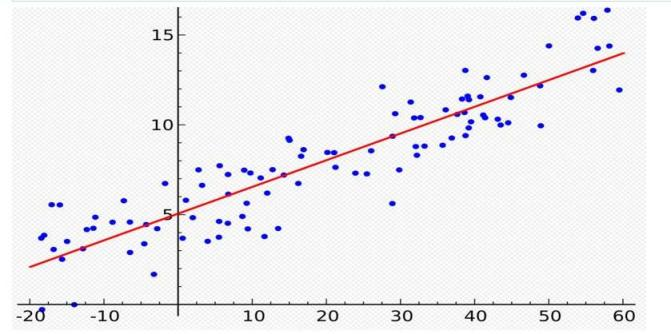
\includegraphics{sLR-Gerade} 
\end{center}
\textbf{k=2:} Das nächste Bild zeigt die $ \color{black}{"Regressionsebene"} $ für die n blauen Beobachtungspunkte $ \color{blue}{\lbrace P_1 = (x_1, y_1, z_1)\quad ... \quad P_n = (x_n, y_n, z_n)\rbrace } $
\begin{center}
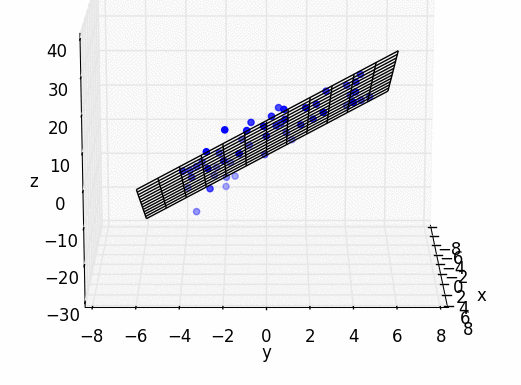
\includegraphics{ML5-MovingPicture_mLR}\
\end{center} 
Ein bewegtes Bild davon liegt in der Referenz [HVö-GitML20]: 
\url{https://github.com/HVoellinger/Lecture-Notes-to-ML-WS2020/blob/master/ML5-QYuIc.gif}
.....\\


\subsection{Kennzahlen  $ R^2 $ und $ Adj.{R^2} $ }
%
Für die Definition der \textbf{{\color{blue}{simple Linear Regression (sLR)}}}\index{Simple Linear Regression (sLR)|hyperpage} und \textbf{{\color{blue}{multiple Linear Regression (mLR)}}} \index{Multiple Linear Regression (mLR)|hyperpage} brauchen wir einige Kennzahlen für die Datenpunkte ("Beobachtungspunkte") aus der  {\color{blue}{Trainingsmenge}}\index{Trainingsmenge} (\textit{observation points).}
Diese Kennzahlen sind \textbf{Sum of Squares Total (SST)},\textbf{ Sum of Squares Error (SSE)} und \textbf{Sum of Squares Regression (SSR)}
%
\subsubsection{Definition der sLR Kennzahl $ R^2 $}
%
Das {\color{blue}{Bestimmtheitsmaß $R^2$}} \index{Bestimmtheitsmaß $R^2$}, auch ”Determinationskoeffizient” (von lateinisch: ”Determination”
”Abgrenzung, Bestimmung“ bzw. ”determinare” ”eingrenzen“, ” festlegen“, ”bestimmen“ und ”coefficere” ”mitwirken“), bezeichnet mit $R^2$, ist in der Statistik eine Kennzahl zur Beurteilung der Anpassungsgüte einer Regressionsanalyse.\\
Das Bestimmtheitsmaß beruht auf der ”Quadratsummenzerlegung”, bei der die totale
Quadratsumme in die durch das Regressionsmodell erklärte Quadratsumme einerseits
und in die Residuenquadratsumme (oder auch ”Fehlerquadratsummen”) andererseits
zerlegt wird.\\[0.2cm]
Weil das Bestimmtheitsmaß durch die Aufnahme zusätzlicher Variablen wächst und
die Gefahr der Überanpassung besteht, wird für praktische Anwendungen meist das
{\color{blue}{adjustierte Bestimmtheitsmaß $Adj.R^2$}} \index{Adjustiertes Bestimmtheitsmaß $Adj.R^2$} verwendet. Das adjustierte Bestimmtheitsmaß bestraft im Gegensatz zum unadjustierten Bestimmtheitsmaß die Aufnahme jeder neu hinzugenommenen abhängigen und unabhängigen Variable.\\[0.2cm]
Die Regressionsgerade $f(x)$ als Schätzer (Modellfunktion) für den Zusammenhang von
Größe und Gewicht der Probanden. $f(xi) = f_i $  ist das geschätzte Gewicht des
Probanden bei einer gegebenen Größe $x_i$.\\[0.2cm]
Der Restfehler (das Residuum) $\varepsilon_i$ stellt die Differenz zwischen dem Messwert $y_i$ und dem Schätzwert $f_i$ dar.\\[0.2cm]
%
Die Definition des {\color{blue}{Bestimmtheitsmaß $R^2$}} \index{Bestimmtheitsmaß $R^2$} benutzt die Kennzahlen SST und SSE). SSR wird für die eigentliche Definition von $R^2$ nicht genutzt. Wir brauchen diese Kennzahl aber später im Kapitel. Sei n = (Anzahl der Beobachtungen) dann definieren wir der Einfachheit halber: 
\begin{center}
$ f_i = f(x_i)\quad $ und $ \quad \overline{x} = \frac{1}{n} \sum\limits_{i=1}^n (x_i) ; \quad \overline{y} = \frac{1}{n} \sum\limits_{i=1}^n (y_i) $\\
\end{center} 
%Mit einfachen Umrechnungen (Matrizenrechnung) zeigt man: \\[0.2cm]
%$ \overline{f}} = \overline{y} $. \\[0.2cm]
%{\color{red}{******* Beweis hier noch einfügen  *******\\
%****** Beweis nutzt Matrixschreibweise *****}}\\\\[0.6cm]
%
SST, SSE und SSR sind gegeben durch die folgenden Definitionen. Ohne Verlust der Allgemeinheit (o.A.) können wir dabei annehmen das SST größer als Null ist:
\begin{center}
$ \texttt{(D-5.1): Sum of Squares Total (SST) := } \sum\limits_{i=1}^n \Bigl(y_i - \overline{y})\Bigr)^2 $ \index{Sum of Squares Total (SST)}
$ \texttt{(D-5.2): Sum of Squares Error (SSE) := } \sum\limits_{i=1}^n \Bigl(y_i - f_i\Bigr)^2 = \sum\limits_{i=1}^n \varepsilon_i^2 $ \index{Sum of Squares Error (SSE)}
$ \texttt{(D-5.3): Sum of Squares Regression (SSR) := } \sum\limits_{i=1}^n \Bigl(f_i - \overline{y})\Bigr)^2 $ \index{Sum of Squares Regression (SSR)} 
\end{center}
% Zeilenfüller
Für die Definition von $R^2$ brauchen wir Sum of Squares Error (SSE) und Sum of Squares Total (SST). Die Definition von $R^2$ ist gegeben durch die Differenz von 1 und dem Quotienten SSE/SST. Wir nennen $R^2$ in Deutsch auch {\color{blue}{"Bestimmtheitsgmaß"}}: \index{Bestimmtheitsmaß $R^2$}\\
\begin{center}
\texttt{(D-5.4):}
\begin{Large}  
\textbf{$ R^2 := 1 - \frac{SSE}{SST} $} \\[0.8cm]
\end{Large}   
\end{center}
% 
\textbf{Anmerkungen und Definition von $MSE$}:\\[0.2cm]
Bei der Nutzung von Python-Programmen, insbesondere bei der Nutzung der NumPy Bibliothek, wird oft noch eine weitere Kennzahl ("Measure") zur Messung der Güte der Regression benutzt. Diese Kennzahl ist  {\color{blue}{"Mean Squared Error" $(MSE)$}} \index{Mean Squared Error (MSE)} und ist eine Abwandlung der Definition von SSE (D-5.2). $ MSE$ ist definiert durch:
\begin{center}
$ \texttt{(D-5.5): Mean Squared Error (MSE) := } \frac{1}{n} \cdot \sum\limits_{i=1}^n \Bigl( y_i - f_i \Bigr)^2 = \frac{1}{n} \cdot \sum\limits_{i=1}^n \varepsilon_i^2 $ \\
\end{center} 
%
\textbf{Erläuterungen zu obigen Definitionen}:\\[0.3 cm]
%
In der einfachen linearen Regression haben die Begriffe SSE, SSR, SST und MSE folgende Bedeutungen:
\begin{itemize}
\item \textbf{SSE (Sum of Squares Error)}:\index{Sum of Squares Error (SSE)} \\ 
SSE steht für die ”Summe der quadrierten Fehler (”Error”)”. In der Literatur wird dies manchmal auch als ”Sum of Squares Residuals” bezeichnet. Wir wählen aber lieber den Begriff ”Error” um auch mit der Abkürzung SSE konsistent zu sein. SSE misst die Gesamtmenge der Abweichungen zwischen den beobachteten Datenpunkten $y_i$ und den vorhergesagten Werten $ f_i $ der Regressionsgeraden. Es repräsentiert die nicht erklärte Variation in den Daten. 
    
\item \textbf{SSR (Sum of Squares Regression)}:\index{Sum of Squares Regression (SSR)} \\
SSR steht für die "Summe der quadrierten Abweichungen der Regression" (Sum of Squares Regression)\index{Sum of Squares Regression (SSR)}. Die SSR misst die Variation, die durch die Regression erklärt wird. Sie quantifiziert die Summe der quadrierten Distanzen zwischen den vorhergesagten Werten \(\hat{y}_i\) und dem Mittelwert \(\bar{y}\) der abhängigen Variable.
    
\item \textbf{SST (Sum of Squares Total)}:\index{Sum of Squares Total (SST)} \\ SST steht für die "Gesamtsumme der quadrierten Abweichungen" (Sum of Squares Total). Die SST misst die Gesamtvariation der beobachteten Werte \(y_i\) um ihren Mittelwert \(\bar{y}\). Es ist die Summe der quadrierten Abweichungen jedes Datenpunkts von \(\bar{y}\).

\item \textbf{MSE (Mean Squared Error)}:\index{Mean Squared Error (MSE)}\\ Die MSE-Kennzahl ist eine weit verbreitete Metrik zur Beurteilung der Güte einer linearen Regression, einem statistischen Verfahren zur Vorhersage von abhängigen Variablen anhand von unabhängigen Variablen. Die MSE-Kennzahl quantifiziert, wie gut die Regressionsgerade die tatsächlichen Datenpunkte approximiert.Insgesamt ist der MSE eine nützliche Kennzahl, um die Genauigkeit eines linearen Regressionsmodells zu bewerten. Es ist jedoch wichtig zu beachten, dass je nach Anwendungsfall auch andere Metriken in Betracht gezogen werden können, um die Vorhersagequalität zu beurteilen.
\end{itemize}
%
Die Beziehung zwischen den Kennzahlen SST, SSE und SSR kann durch die Gleichung \(SST = SSR + SSE\) für optimale Regressionsgeraden ausgedrückt werden. Diese Gleichung zeigt, wie die Gesamtvariation der abhängigen Variable in die Variation, die durch die Regression erklärt wird (SSR), und die nicht erklärte Variation (SSE) aufgeteilt wird.\\[0.2 cm]
% 
\textbf{Sprechweise:} Wir sagen eine Gerade ist eine \textbf{"optimale"} (sLR)-Gerade wenn R² maximal ist (dies ist analog zu SSE ist minimal). Oftmals wird in der Literatur auch der Zusatz "optimale" weggelassen und man sagt nur "sLR-Gerade".\\[0.4 cm]
% 
%\textbf{Anmerkung:} Wir sehen später das für  optimale sLR-Geraden eine andere Formel für R² auch gültig ist. Diese Formel benutzt die Kennzahl SSR.\\[0.4cm]
% 
Im \textbf{folgenden Bild} sehen wir die Kennzahlen {\color{blue}{SSE}} und {\color{red}{SST}} geometrisch mit 4 Beobachtungspunkten. Sehr gut sind die Größen der Quadrate für {\color{blue}{SSE}} und {\color{red}{SST}} zu erkennen. Man bekommt zudem auch ein guten Eindruck von den Faktor 
\begin{large}
$ \frac{\color{blue}{SSE}}{\color{red}{SST}} $.\\[8.8cm]
\end{large}
%
\begin{figure}[htp]
\hspace*{-0.2cm}  
\centering 
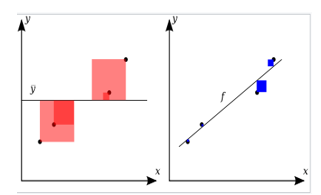
\includegraphics[width=0.8\textwidth]{SSE_SST-Definition}
  \caption{Geometrische Darstellung von {\color{blue}{SSE}} und {\color{red}{SST}}}
  \label{fig:SSE-SST-1}
\end{figure}
%
\subsubsection{Eigenschaften und Theoreme zu $R^2$ $(k \geqslant 2$ } 

Nun wollen wir die ersten offensichtlichen mathematische Aussagen zu R² machen. \\
Zur leichteren Schreibweise nutze ich die folgenden Notationen:\\
\begin{center}
sum(xi) := $ \sum\limits_{i=1}^n(x_i) $  und  $ \overline{x} := \frac{1}{n} \cdot \sum\limits_{i=1}^n(x_i) $\\[0.2cm]
\end{center}
Wir beginnen mit einigen einfachen mathematischen Aussagen ("Theoreme", "Propositionen", "Korollare", etc. ) über die Eigenschaften der Kennzahl $R^2$.\\[0.2cm]
\textbf{Anmerkung:} Ohne Einschränkung der Allgemeinheit ("OE") können wir annehmen, dass $SST > 0$ ist.\\[0.2cm] 
%
\textbf{Theorem (Th-5.1)}: "Eigenschaften von $R^2$”\\[0.2cm]
Es gelten die folgenden Aussagen:\\[0.3cm]
(i)  $ \quad 0 \leqslant R^2 \leqslant 1 \quad\quad\quad\quad\quad\quad $   "Begrenzung"\\[0.2cm]                                       
(ii) $ \quad R^2 = 0 \Leftrightarrow SSE = SST \quad $                      "Minimum"\\[0.2cm]                                       
(iii) $ \quad R^2 = 1 \Leftrightarrow SSE = 0 \quad\quad\quad $                 "Maximum"\\[0.4cm]                                       
\textbf{Beweis:}
Der Beweis dieser Aussagen ist trivial. Um aber das mathematische Kalkül einzuüben führen wir hier die mathematische Beweisargumentation explizit aus:\\[0.2cm]
ad (i): per Definition gilt $ SST \geqslant SSE \Leftrightarrow 1 \geqslant \frac{SSE}{SST} \Leftrightarrow 1- \frac{SSE}{SST} \geqslant 0 \Leftrightarrow R^2\geqslant 0 $\\[0.2cm]                                       
per Definition gilt $ \frac{SSE}{SST} \geqslant 0 \Leftrightarrow 0 \geqslant -\frac{SSE}{SST} \Leftrightarrow 1 \geqslant 1- \frac{SSE}{SST} \frac{SSE}{SST} R^2 \leqslant 1 $ \\[0.3cm]                                       
ad (ii): $ SSE = SST \Leftrightarrow \frac{SSE}{SST} = 1 \Leftrightarrow 1 - \frac{SSE}{SST} = 0 \Leftrightarrow R^2 = 0 $ \\[0.2cm]                                                                           
ad (iii): $SSE = 0 \Leftrightarrow \frac{SSE}{SST} = 0 \Leftrightarrow  1 + \frac{SSE}{SST} = 1 \Leftrightarrow  1 = 1 -  \frac{SSE}{SST} \Leftrightarrow  R^2 = 1 \qquad $ q.e.d. \\[0.3cm] 
%
Manchmal ist es notwendig das die optimale sLR-Gerade durch den Ursprung (a=0) geht. In diesem Fall erhalten wir die folgende Aussage:\\
\\[0.2cm]
\textbf{Korollar(K-5.1)}: “opt. sLR ohne Achsenabschnitt(a =0)”\\
\begin{center}
\begin{large}
Aus $ a=0 \Rightarrow b = {\dfrac{\overline{x \cdot y}}{\overline{x^2}}}$  \\[0.2cm]                                          
\end{large}
\end{center}
\textbf{Beweis:}\\
$ a = 0 \Rightarrow y = b \cdot x$\\\\[0.1cm]
%                                                                           
Da die sLR-Gerade optimal ist, muss die Ableitung von $R^2$ nach b gleich Null. Berechne nun diese. Da die Ableitung von SST konstant ist und die Gleichung später = 0 gesetzt wird, gilt: 
\begin{center}
\begin{large}
$ 0 =\frac{\partial}{\partial b} (1-\frac{SSE}{SST}) = \frac{\partial)}{\partial b} [SSE] = \frac{\partial}{\partial b}[\sum\limits_{i=1}^n [(y_i - b \cdot x_i)^2] = -2 \cdot \sum(y_i \cdot x_i - b \cdot (x_i)^2) $ 
\end{large}
\end{center}
daraus folgt:
\begin{center}
\begin{large}
$ \sum(y_i \cdot x_i) =  b \cdot \sum(x_i)^2) \Rightarrow b = \frac{\sum(y_i \cdot x_i) }{\sum(x_i)^2)} \Rightarrow m = \frac{\overline{x \cdot y}}{\overline{x^2}} \qquad $ q.e.d.     \\[0.5cm] 
\end{large}
\end{center} 
%
Wir brauchen für später auch noch weitere hilfreiche Formeln über Summen und Mittelwerte. Diese werden für die Berechnung der “optimalen” Koeffizienten $a$ und $b$ gebraucht (siehe: “Least Square Fit” (LSF) Methode):\\[0.8cm]
%                                                                                                                                     
\textbf{Proposition (P-5.1)}:\\[0.2cm]
%
Leicht können dann die folgenden 3 Aussagen bewiesen werden: \\
\begin{enumerate}
 \item  $ \quad (i:) \quad \sum(x_i - \bar{x})^2 = \sum(x_i^2) - n \cdot \bar{x}^2 $\\[0.2cm] 
    
 \item  \( \quad (ii:) \quad \sum(y_i - \bar{y})^2 = \sum(y_i^2) - n \cdot \bar{y}^2\)\\[0.2cm] 
    
 \item  \( \quad (iii:) \quad \sum((x_i - \bar{x}) \cdot (y_i - \bar{y})) = \sum(x_i \cdot y_i) - n \cdot \bar{x} \cdot \bar{y} \)\\[0.2cm] 
\end{enumerate}

\textbf{Beweis:}\\[0.1cm]
"straightforward":

\begin{enumerate}
    \item \( \sum(x_i - \bar{x})^2 = \sum(x_i^2 - 2 \cdot \bar{x} \cdot x_i + \bar{x}^2) \) \\[0.2cm]
        \(= \sum(x_i^2) - 2 \cdot \bar{x} \cdot \sum(x_i) + \sum(\bar{x}^2)\)\\[0.2cm]
        \(= \sum(x_i^2) - 2 \cdot n \cdot \bar{x}^2 + n \cdot \bar{x}^2 \quad \) ( weil:  \(\sum(x_i) = n \cdot \bar{x} \))\\[0.2cm]
        
    \item Analog: \(\sum(y_i - \bar{y})^2) = \sum(y_i^2) - n \cdot \bar{y}^2\)\\[0.2cm]
    
    \item Analog: \( \sum((x_i - \bar{x})(y_i - \bar{y})) = \sum(x_i \cdot y_i) - n \cdot \bar{x} \cdot \bar{y} \quad \)   q.e.d. \\[0.3cm]
\end{enumerate}   
%     
\subsubsection{Definition der mLR-Kennzahl Adj.R²}
%
In diesem Abschnitt definieren wir die Theorie der \href{https://en.wikipedia.org/wiki/Linear_regression}{"mutiple linear regression"}.\\
In einem {\color{blue}{multiplen Regression Problem}} arbeiten wir mit $n$ Datenpaaren $\langle\mathbf{x}^{(i)}, y^{(i)} \rangle \in \mathbb{R}^{k+1} $ 
wobei $\mathbf{x}^{(i)} \in \mathbb{R}^k$ und $y^{(i)} \in \mathbb{R}$ für alle $i \in \{1,\cdots,n\}$.  \\
Die Zahl $k$ ist die Anzahl der unabhängigen {\color{blue}{Features ("Prädiktoren") $ {\mathbf{x}^{(i)}} $ } }, und {\color{blue}{$ y^{(i)}$}} ist die abhängige {\color{blue}{Zielvariable ("target column")}}. Die Datenpaare nennen wir auch {\color{blue}{Trainings-Menge}}\index{Trainingsmenge}. Unser Ziel ist es die folgende Funktion:  
\\[0.2cm]
\hspace*{1.3cm}
\begin{large}
$F:\mathbb{R}^k \rightarrow \mathbb{R}$ 
\end{large} 
zu berechnen, so dass 
\\[0.2cm]  
$ F\bigl(\mathbf{x}^{(i)}\bigr)$ eine  genaue Approximation von $y^{(i)}$ ist,  für alle for all $i\in\{1,\cdots,n\}$, insbesondere wollen wir erreichen: \\[0.3cm]
\hspace*{1.3cm}
\begin{large}
$\forall i\in\{1,\cdots,n\}:F\bigl(\mathbf{x}^{(i)}\bigr) \approx y^{(i)}$. \\[0.4cm]
\end{large}
%
Die {\color{blue}{Kennzahl $Adj.R^2$}}\index{Adjustiertes Bestimmtheitsmaß $Adj.R^2$}, wobei "Adj." für "Adjustiert" (angepasst) steht, soll nun genauer definiert werden. Die Adj.R² ist eine modifizierte Version des gewöhnlichen R² ("Bestimmtheitsmaß").\\
Während das normale R² die Proportion der abhängigen Variabilität erklärt, kann das Adj.R² bei Modellen mit mehreren unabhängigen Variablen ("Prädiktoren") nützlicher sein, da es für die Anzahl der verwendeten Prädiktoren oder Kovariaten in einem Modell nutzt.\\
Bezeichnen wir n = Anzahl der Beobachtungen (Datenpunke) und k = Anzahl der unabhängigen Variablen (Prädiktoren) und definieren wir df := n-k-1 ("Anzahl der Freiheitsgrade"). Dann ergibt sich, unter Nutzung von (D-5.4), folgende Formel:\\[0.1cm]

\begin{center}
\texttt{(D-5.5)}
\begin{large}
\textbf{$ \quad Adj.R^2 := 1 - (1 - R^2) \cdot (\frac{n-1}{n-k-1}) = 1 - (\frac{SSE}{SST}) \cdot (\frac{n-1}{n-k-1}) $}  \\[0.6cm] 
\end{large}     
\end{center}
%
Das Adj.R² berücksichtigt die Anzahl der unabhängigen Variablen ("Prädiktoren") im Modell und passt das gewöhnliche R² an, um zu verhindern, dass es aufgrund von Überanpassung ("Overfitting") zu optimistisch wird. Ein höheres Adj.R² zeigt an, dass ein größerer Anteil der Variabilität im abhängigen Wert von den unabhängigen Variablen im Modell erklärt wird, wobei jedoch die Anzahl der Prädiktoren berücksichtigt wird. Zusammenfassend ergibt sich folgende Übersicht:\\

\begin{center}
\includegraphics{Adj.R²-Definition}\\
\end{center}
%
\textbf{Sprechweise:} Wir sagen eine Hyperebene ist eine \textbf{"optimale"} (mLR)- Hyperebene wenn Adj.R² maximal ist (dies ist analog zu SSE ist minimal). Oftmals wird in der Literatur auch der Zusatz "optimale" weggelassen und man sagt nur "mLR-Hyperebene".\\ 




\subsection{"Least Square Fit"(LSF) Verfahren für LR}

Mit den LSF Verfahren oder in Deutsch "Methode der kleinsten Quadrate" lassen sich nun die optimale sLR-Gerade (k=1) und im Fall (k=2) die optimale mLR-Ebene berechnen. Wir nutzen das "Max-Min" Kriterium der Analysis.\\
Wir berechnen dazu explizit die Ableitung der Funktion R² nach ihren Veränderlichen in den Fälle (k=1)und (k=2).\\
Um dies Durchführen zu können brauchen wir noch einige mathematische Grundlagen der Matrizenrechnung aus der Linearen Algebra. Dies sind die Berechnung einer Inversen einer Matrix \index{Inverse} und die Berechnung der Determinante\index{Determinante} einer Matrix. Beispielhaft zeigen wir jetzt nur die Formel für die Berechnung einer Determinante. Der Rest ist Wiederholung der Linearen Algebra Vorlesung.
%
\subsubsection{Lineare Algebra - Inverse und Determinante einer Matrix}
In diesem Unterkapitel machen wie eine kleine Wiederholung der Vorlesung über Lineare Algebra. Wir definieren die Inverse und die Determinante einer Matrix und geben ein Beispiel dazu. \\[0.3cm]
\textbf{Berechnung der Inversen Matrix $A^{-1}$}\\[0.2cm]
Du kannst die Matrixgröße und die Elemente entsprechend deiner spezifischen Matrix anpassen. Die inverse Matrix von $A$:
\[
A = \begin{bmatrix}
    a_{11} & a_{12} & \cdots & a_{1n} \\
    a_{21} & a_{22} & \cdots & a_{2n} \\
    \vdots & \vdots & \ddots & \vdots \\
    a_{n1} & a_{n2} & \cdots & a_{nn} \\
\end{bmatrix}
\]
kann mit der Formel
\begin{large}
\\[0.5cm]
\hspace*{4.0cm}
\colorbox{blue}{\framebox{\colorbox{yellow}{
$ A^{-1} = \frac{1}{\text{det}(A)} \cdot \text{adj}(A) $
}}} $ \qquad \qquad \qquad \quad $ (Inv)\\[0.6cm]
\end{large}
% 
berechnet werden, wobei $\text{adj}(A)$ die adjungierte (auch bekannt als die adjazente oder komplementäre) Matrix von $A$ ist.\\
%
Die adjungierte Matrix von $A$ (oft als $\text{adj}(A)$ abgekürzt) wird berechnet, indem man die Kofaktormatrix transponiert:
\[
\text{adj}(A) = \begin{bmatrix}
    C_{11} & C_{21} & \cdots & C_{n1} \\
    C_{12} & C_{22} & \cdots & C_{n2} \\
    \vdots & \vdots & \ddots & \vdots \\
    C_{1n} & C_{2n} & \cdots & C_{nn} \\
\end{bmatrix}
\]
\\[0.4cm]
wobei $C_{ij}$ die Kofaktoren der Elemente von $A$ sind. Die Kofaktoren werden durch das Entfernen der i-ten Zeile und j-ten Spalte aus $A$ und berechnen der Determinante\index{Determinante} der verbleibenden (n-1)x(n-1)-Matrix erhalten.\\[0.8cm]
%
\textbf{Berechnung der Determinante $det(A)$}\\[0.2cm]
Die Determinante von  einer (nxn)-Matrix $A$ wird bezeichnet durch folgende {Notation:\footnote{Senkrechte  Striche vor und hinter der Matrix $A$ bedeutet Determinante von $A$}}
\[
\begin{vmatrix}
    a_{11} & a_{12} & \cdots & a_{1n} \\
    a_{21} & a_{22} & \cdots & a_{2n} \\
    \vdots & \vdots & \ddots & \vdots \\
    a_{n1} & a_{n2} & \cdots & a_{nn} \\
\end{vmatrix}
\]
\\[0.4cm]
und kann mit dieser allgemeinen Formel berechnet werden:
\begin{large}
\\[0.5cm]
\hspace*{3.0cm}
\colorbox{blue}{\framebox{\colorbox{yellow}{
$ \text{det}(A) = \sum_{i=1}^{n} (-1)^{i+j} \cdot a_{ij} \cdot \text{det}(A_{ij})$
}}} $ \qquad $ (Det-1)\\[0.5cm]
\end{large}
wobei $A_{ij}$ die Matrix ist, die durch Entfernen der i-ten Zeile und j-ten Spalte aus $A$ entsteht.\\[0.8cm]
\textbf{Bemerkung: Definition der Determinante nach Leibniz (1690):}\\[0.4cm]
In dieser Bemerkung definieren wir etwas allgemeiner und eleganter die \href{https://de.wikipedia.org/wiki/Determinante}{Determinante} einer $n \times n$ Matrix so, wie dies 1690 von \href{http://de.wikipedia.org/wiki/Gottfried_Wilhelm_Leibniz}{Gottfried Wilhelm Leibniz\footnote{G. W. Leibniz war einer der bekanntesten Mathematiker, Philosophen und Naturwissenschafter seiner Epoche.}} vorgeschlagen wurde. Wir verzichten hier aus Zeitgründen auf die Einführung von Permutationsgruppen. Dies kann auch in Wikipedia leicht nachgeschaut werden.\\[0.2cm]
Ist $A = (a_{i,j}) \in \mathbb{K}^{n \times n}$, wobei entweder 
$\mathbb{K}= \mathbb{R}$ oder $\mathbb{K}= \mathbb{C}$ gilt, so definieren wir die {\emph{\color{blue}Determinante}} von $A$ (geschrieben $\mathtt{det}(A)$) über die Formel:
\begin{large}
\\[0.6cm]
\hspace*{0.0cm}
\colorbox{blue}{\framebox{\colorbox{yellow}{
$\texttt{det}(A =  \sum\limits_{\sigma \in \mathcal{S}_n} \texttt{sgn}(\sigma) \cdot \prod\limits_{i=1}^n a_{i,\sigma(i)} 
 = \sum \Bigl\{ \texttt{sgn}(\sigma) \cdot  \prod\limits_{i=1}^n a_{i,\sigma(i)} \Bigm| \sigma \in \mathcal{S}_n \Bigr\} $
}}} \\ $ \qquad $(Det-2)\\[0.6cm]
\end{large}
%
\textbf{Beispiel für eine $2 \times 2$ Matrix:}\\[0.2cm]
Es sei $A$ eine $2 \times 2$ Matrix, es gilt also
\\[0.2cm]
\hspace*{1.3cm}
$A = \left(
  \begin{array}{ll}
    a_{1,1} & a_{1,2} \\[0.2cm] 
    a_{2,1} & a_{2,2} 
  \end{array}
  \right)
$
\\[0.2cm]
Zur Berechnung von $\texttt{det}(A)$ (nach Leibniz, Formel (Det-2)) müssen wir uns überlegen, wie $ \mathcal{S}_2 $ aussieht.  Es gilt
\\[0.2cm]
\hspace*{1.3cm}
$\mathcal{S}_2 := \bigl\{ [1,2], [2,1] \bigr\}$.
\\[0.2cm]
Für die Permutation $[1,2]$ finden wir:  $\texttt{sgn}([1,2]) = (-1)^0 = +1$.
\\[0.2cm]
Und für die  Permutation $[2,1]$ ergibt sich: $ \quad \texttt{sgn}([2,1]) = (-1)^1 = -1 $.
\\[0.2cm]
Insgesamt haben wir
\\[0.2cm]
\hspace*{0.3cm}
$\texttt{det}(A) = \texttt{det}\left(\begin{array}{ll}
    a_{1,1} & a_{1,2} \\[0.2cm] 
    a_{2,1} & a_{2,2} 
  \end{array}
  \right)
  = (+1) \cdot a_{1,1} \cdot a_{2,2} + (-1) \cdot a_{1,2} \cdot a_{2,1} 
  = a_{1,1} \cdot a_{2,2} - a_{1,2} \cdot a_{2,1} $
Somit ergibt sich mit der Formel (Inv):\\[0.2cm]  
$ A^{-1} = \frac{1}{det A} \cdot \left(
  \begin{array}{ll}
    a_{2,2} & - a_{2,1} \\[0.2cm] 
    - a_{1,2} & a_{1,1} 
  \end{array}
  \right)
$ 
\\[0.4cm]
Es wird empfohlen bei solchen Rechnungen immer eine Probe zu machen, indem man jetzt mit den konkreten Werten die Gleichung: $A \cdot A^{(-1)} = E (Einheitsmatrix)$ nachrechnet.\\[0.3cm]
%
\textbf{Beispiel für eine $3 \times 3$ Matrix:}\\[0.2cm]
Für eine $3 \times 3$ Matrix $A$ lassen sich Inverse und Determinante analog berechnen.\\ Eine manuelle Berechnung ist jedoch sehr aufwendig und es ist ratsam einen entsprechenden ML Algorithmus zu benutzen. Du kannst dazu etwa  Jupyter Notebook ausführen. Stelle sicher, dass die benötigte NumPy-Bibliothek installiert ist. Im entsprechenden Codebeispiel (weiter unten) entwickeln wird ein Notebook erstellt, dass für eine symmetrische 3x3-Matrix A, ihre Determinante und Adj. Matrix berechnet, woraus sich die inverse Matrix von A sich ergibt.\\
Gegeben sei die 3x3-Matrix $A$:
\[
A = \begin{bmatrix}
    a_{11} & a_{12} & a_{13} \\
    a_{21} & a_{22} & a_{23} \\
    a_{31} & a_{32} & a_{33} \\
\end{bmatrix}
\]
Berechnung der adjungierten Matrix $\text{adj}(A)$:
\[
\text{adj}(A) = \begin{bmatrix}
    C_{11} & C_{21} & C_{31} \\
    C_{12} & C_{22} & C_{32} \\
    C_{13} & C_{23} & C_{33} \\
\end{bmatrix}
\]
wobei $C_{ij}$ die Kofaktoren der Elemente von $A$ sind:
\[
C_{11} = \begin{vmatrix}
    a_{22} & a_{23} \\
    a_{32} & a_{33} \\
\end{vmatrix}, \quad
C_{12} = -\begin{vmatrix}
    a_{21} & a_{23} \\
    a_{31} & a_{33} \\
\end{vmatrix}, \quad
C_{13} = \begin{vmatrix}
    a_{21} & a_{22} \\
    a_{31} & a_{32} \\
\end{vmatrix}
\]
\[
C_{21} = -\begin{vmatrix}
    a_{12} & a_{13} \\
    a_{32} & a_{33} \\
\end{vmatrix}, \quad
C_{22} = \begin{vmatrix}
    a_{11} & a_{13} \\
    a_{31} & a_{33} \\
\end{vmatrix}, \quad
C_{23} = -\begin{vmatrix}
    a_{11} & a_{12} \\
    a_{31} & a_{32} \\
\end{vmatrix}
\]
\[
C_{31} = \begin{vmatrix}
    a_{12} & a_{13} \\
    a_{22} & a_{23} \\
\end{vmatrix}, \quad
C_{32} = -\begin{vmatrix}
    a_{11} & a_{13} \\
    a_{21} & a_{23} \\
\end{vmatrix}, \quad
C_{33} = \begin{vmatrix}
    a_{11} & a_{12} \\
    a_{21} & a_{22} \\
\end{vmatrix}
\]
Die Kofaktoren werden durch die Berechnung der Determinanten von 2x2-Untermatrizen erstellt. Du kannst die Werte der Matrix $A$ anpassen, um die Kofaktoren und die adjungierte Matrix für deine spezifische Matrix zu berechnen.\\[0.4cm]
Berechnung der Determinante $\text{det}(A)$:
\[
\text{det}(A) = a_{11} \cdot \begin{vmatrix}
    a_{22} & a_{23} \\
    a_{32} & a_{33} \\
\end{vmatrix} - a_{12} \cdot \begin{vmatrix}
    a_{21} & a_{23} \\
    a_{31} & a_{33} \\
\end{vmatrix} + a_{13} \cdot \begin{vmatrix}
    a_{21} & a_{22} \\
    a_{31} & a_{32} \\
\end{vmatrix}
\]
Berechne die Determinanten der 2x2-Untermatrizen, indem du die Differenz der Produkte der Hauptdiagonalen und Nebendiagonalen verwendest:
\[
\text{det}(A) = a_{11} \cdot ((a_{22} \cdot a_{33}) - (a_{23} \cdot a_{32})) - a_{12} \cdot ((a_{21} \cdot a_{33}) - (a_{23} \cdot a_{31})) + a_{13} \cdot ((a_{21} \cdot a_{32}) - (a_{22} \cdot a_{31}))
\]
%
\textbf{Beispiel für eine symmetrische $3 \times 3$ Matrix:}\\[0.2cm]
In diesem Beispiel wird die Inverse\index{Inverse} und Determinante der 3x3-Matrix $A$ mithilfe des Laplace'schen\footnote{Pierre-Simon Laplace war einer der führenden Mathematiker und Wissenschaftler des 18. und 19. Jahrhunderts und hinterließ einen erheblichen Einfluss auf verschiedene Bereiche der Mathematik und Naturwissenschaften.} Entwicklungssatzes berechnet.\\
Dieser Satz ermöglicht es, die Determinante einer Matrix durch die Berechnung von Determinanten kleinerer Matrizen zu finden, was besonders nützlich ist, wenn die Matrix groß ist. \\
Um die Inverse einer Matrix zu berechnen, könnte man den Laplace-Entwicklungssatz verwenden, um die Determinante der Matrix zu finden und dann die Cofaktormethode oder eine andere Methode zur Berechnung der Inversen anwenden. \\
Du kannst die Werte der Matrix $A$ anpassen, um die Determinante für deine spezifische Matrix zu berechnen.\\[0.2cm]
Ist die Matrix \textbf{symmetrisch} so vereinfachen sich die Formel wesentlich. Gegeben sei die symmetrische 3x3-Matrix $A$:
\[
A = \begin{bmatrix}
    a & b & c \\
    b & d & e \\
    c & e & f \\
\end{bmatrix}
\]
Um die inverse Matrix $A^{-1}$ zu berechnen, führen wir die folgenden Schritte aus:\\[0.2cm]

1. Berechne die Determinante von $A$:
\[
\text{det}(A) = a(df - ce) - b(ef - cd) + c(be - dc)
\]
2. Berechne die Kofaktoren der Matrix $A$:
\[
\begin{aligned}
C_{11} &= \begin{vmatrix}
    d & e \\
    e & f \\
\end{vmatrix} = df - e^2, \\
C_{12} = C_{21} &= -\begin{vmatrix}
    b & c \\
    e & f \\
\end{vmatrix} = -bf + ce, \\
C_{13} = C_{31} &= \begin{vmatrix}
    b & d \\
    c & e \\
\end{vmatrix} = be - dc, \\
C_{22} &= \begin{vmatrix}
    a & c \\
    c & f \\
\end{vmatrix} = af - c^2, \\
C_{23} = C_{32} &= -\begin{vmatrix}
    a & b \\
    c & e \\
\end{vmatrix} = -ae + bc, \\
C_{33} &= \begin{vmatrix}
    a & b \\
    b & d \\
\end{vmatrix} = ad - b^2.
\end{aligned}
\]
3. Erstelle die adjungierte Matrix $\text{adj}(A)$ durch Transposition der Kofaktormatrix:
\[
\text{adj}(A) = \begin{bmatrix}
    C_{11} & C_{21} & C_{31} \\
    C_{12} & C_{22} & C_{32} \\
    C_{13} & C_{23} & C_{33} \\
\end{bmatrix}
\]
4. Berechne die inverse Matrix $A^{-1}$, indem du $\text{adj}(A)$ durch die Determinante von $A$ teilst:
\[
A^{-1} = \frac{1}{\text{det}(A)} \cdot \text{adj}(A)
\]
Die inverse Matrix $A^{-1}$ ist dann die resultierende 3x3-Matrix.\\
Dieser LaTeX-Code zeigt die korrekte Berechnung der inversen Matrix für die gegebene symmetrische 3x3-Matrix A unter Verwendung des Laplace'schen Entwicklungssatzes (siehe oben).\\[0.4cm]
Auch hier wird empfohlen bei dieser Rechnung eine Probe zu machen, indem man jetzt mit den konkreten Werten die Gleichung: $A \cdot A^{(-1)} = E (Einheitsmatrix)$ nachrechnet.\\[0.3cm]
%
\textbf{Python-Programm zur Berechnung der obigen Inversen:}\\[0.2cm] 
%
Wir entwickeln ein Python Programm als Jupyter Notebook. Du kannst dieses Code-Snippet in einem Jupyter Notebook ausführen. Importiere die benötigte NumPy-Bibliothek.\\ 
Das Notebook erstellt eine symmetrische 3x3-Matrix A, berechnet Det(A) und Adj(A), woraus sich Inv(A) ergibt. Insgesamt besteht das Programm aus 4 Schritten. 
\begin{center} 
\hspace*{-0.5cm}
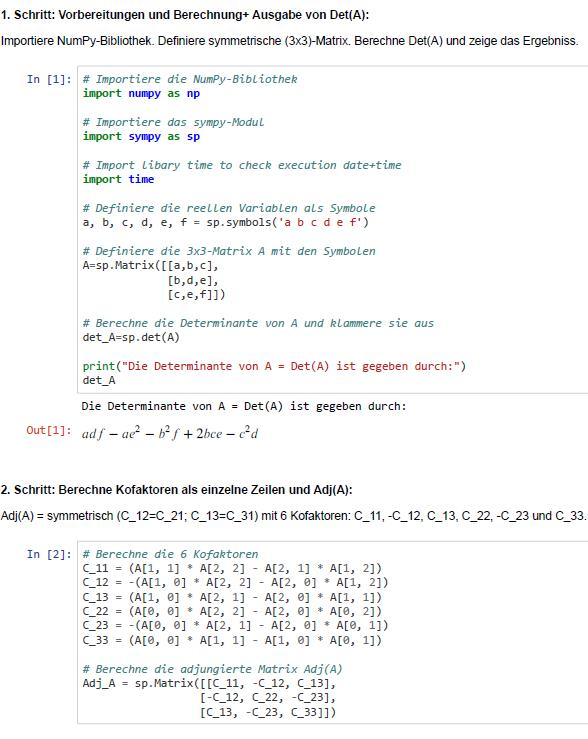
\includegraphics[width=1.12\textwidth]{Inv_Matrix-Step1+2}
\hspace*{-1.0cm} 
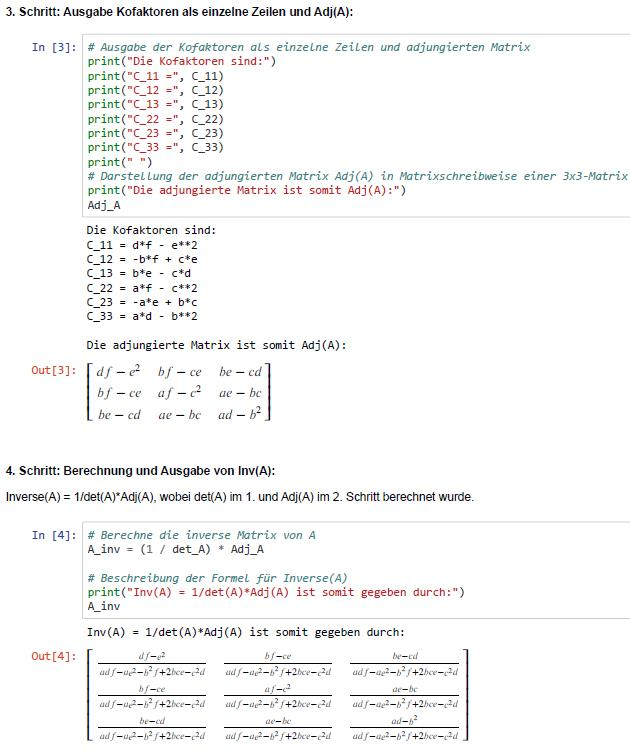
\includegraphics[width=1.15\textwidth]{Inv_Matrix-Step3+4}
\end{center}
%
% \begin{figure}[h]
%  \centering
%  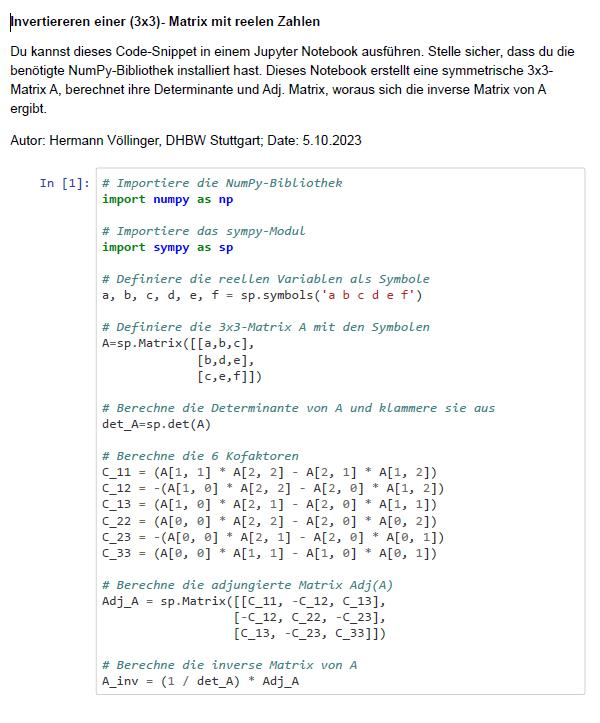
\includegraphics[width=1.0
%  \textwidth]{Inv_Matrix-Berech}
%  \caption{Python-Inv(A)- Berechnung}
%  \label{fig:IVM_Ber}
%\end{figure}
%\\[0.1cm]
%\begin{figure}[h]
%  \centering
%  \includegraphics[width=1.0
%  \textwidth]{Inv_Matrix-Ausgabe}
%  \caption{Python-Inv(A)- Ausgabe}
%  \label{fig:IVM_Ber}
%\end{figure}
%
\subsubsection{Detailberechnung für sLR}
%
Sei die optimale Regression-Gerade gegeben durch $ y = a + b \cdot x $ dann ist R² eine Funktion in den Veränderlichen $a$ und $ b: " R^2 = R^2(a,b)" $. Somit muss für ein Maximum gelten, dass der Gradient $\Delta{R^2}$ = 0 ist (Analysis I): 
\begin{center}
\begin{large} 
$  dR^2 = \frac{\partial R^2}{\partial a} \cdot da + \frac{\partial R^2}{\partial b} \cdot db = 0 \Longleftrightarrow  \frac{\partial R^2}{\partial a} = \frac{\partial R^2}{\partial b} = 0 $
\end{large}
\end{center}
%
Wir rechnen als erstes die \textbf{Ableitung nach $a$}:
% 
\begin{center}
\begin{large} 
$ \frac{\partial R^2}{\partial a} = \frac{\partial}{\partial a}(1 - \frac {SSE}{SST})]  =  \frac{\partial}{\partial a}(1) - \frac{\partial}{\partial a}(\frac{SSE}{SST})= 0 -  \frac{\partial}{\partial a}(SSE) $ 
\end{large}
\end{center}
% 
Die letzte Gleichung ist gültig, da das Gesamtergebnis ebenfalls = 0 gesetzt wird und $ \frac{\partial}{\partial a}(\frac{1}{SST}) = const. $ ist. Damit kann diese Ableitung vernachlässigt werden. Somit erhält man: \\ 

\begin{center}
\begin{large} 
$ 0 = \frac{\partial}{\partial a}(SSE) = \frac{\partial}{\partial a}[\sum\limits_{i=1}^n {((y_i - a -b \cdot x_i)^2)} = -(2) \cdot (\sum\ (y_i - a - b \cdot  x_i)) $
\end{large}
\end{center}
%
Durch Benutzung der Definition des Mittelwertes und Kürzen mit (-2) erhält man: 

\begin{center}
$ 0 = n \cdot \bar{y} - n \cdot a -n \cdot b \cdot \bar{x} \quad \Leftrightarrow \quad 0 = \bar{y} - a  -b \cdot \bar{x}$ \\[0.2cm] 
$ \qquad \qquad \Leftrightarrow \quad a = \bar{y} -b \cdot \bar{x} \qquad\ \Leftrightarrow \quad \bar{y} = a +  b \cdot \bar{x} \qquad $ (1)
\end{center}

Analog berechnen wir die \textbf{Ableitung nach $b$}:
 
\begin{center}
\begin{large} 
$ \frac{\partial R^2}{\partial b} = \frac{\partial [ 1 - \frac {SSE}{SST}]}{\partial b} =  \frac{\partial 1}{\partial b} - \frac{\partial [\frac{1}{SST}]}{\partial b} \cdot \frac{\partial SSE}{\partial b} = 0 -  \frac{\partial [\frac{1}{SST}]}{\partial b} \cdot \frac{\partial SSE}{\partial b} $ 
\end{large}
\end{center}
% 
Da diese Gleichung = 0 gesetzt wird und $ \frac{\partial [\frac{1}{SST}]}{\partial b} = const. $ ist, kann diese Ableitung vernachlässigt werden. Somit erhält man: 

\begin{center}
\begin{large} 
$ 0 = \frac{\partial (SSE)}{\partial b } = \frac{\partial}{\partial b} \dot  [\sum\limits_{i=1}^n [(y_i - a -b \cdot x_i^2] = -2 \cdot \sum[y_i \cdot x_i - a \cdot x_i - b \cdot x_i^2)] $
\end{large}
\end{center}
%
Durch Benutzung der Definition des Mittelwertes und Kürzen durch (-2) erhält man:  
 
\begin{center}
$ 0 = \sum(y_i \cdot x_i) - a \cdot n \cdot \bar{x} - b \cdot \sum(x_i^2) $ \\[0.4cm]  
$ \quad\quad\quad \Leftrightarrow \qquad \sum(y_i \cdot x_i) =  a \cdot n \cdot \bar{x} + b \cdot \sum(x_i^2)\qquad\qquad  $ (2) \\[0.3cm]
\end{center}
%
Schreiben wir nun die beiden Gleichungen (1) und (2) mit einer 2x2- Matrix um, so erhält man nach den Regeln der Matrizenmultiplikation (siehe Vorlesung "Lineare Algebra"):\\[0.2cm]  
\begin{center}
\begin{large} 
$ \begin{bmatrix} 1 & \bar{x} \\ n \cdot \bar{x} & \sum{x_i^2} \\ \end{bmatrix} \cdot                                                                                                  \begin{bmatrix} a \\ b \\ \end{bmatrix} = \begin{bmatrix} \bar{y} \\ \sum{x_i \cdot y_i}  \\ \end{bmatrix} $
\end{large}
\end{center}
%
In der Lin. Algebra wird die Inverse einer 2x2- Matrix:    
A = $ \begin{bmatrix} a & b \\ c & d \\ \end{bmatrix} $ berechnet als: 
\begin{center}
\begin{large} 
$ A^{-1} = \frac{1}{ad - bc} \begin{bmatrix}
d & -b \\
-c & a \\
\end{bmatrix} $
\end{large}
\end{center} 
wobei Determinante(A)= detA = ad - bc. Mit obigen Werten eingesetzt erhält man: \\
\begin{center}
\begin{large}
$ det = \sum{x_i^2} - n \cdot \bar{x}^2 $    (3) \\[0.5cm]        
$ \qquad\qquad  \begin{bmatrix} a \\ b \\ \end{bmatrix} = \frac{1}{det} \cdot { \begin{bmatrix} \sum{x_i^2} & -\bar{x} \\ -n \cdot \bar{x} & 1 \\ \end{bmatrix} \cdot                                                                                                     \begin{bmatrix} \bar{y} \\ \sum{x_i \cdot y_i} \\ \end{bmatrix}} $ \\[0.8cm]
\end{large}
\end{center} 
Unter Berücksichtigung von ($ det = \sum{x_i^2} - n \cdot \bar{x}^2 $) ist dies äquivalent zu den folgenden zwei Formeln : \\
\begin{center}
\begin{Large}
$ a = \frac{1}{det} \cdot (\bar{y} \cdot \sum{x_i^2} - \bar{x} \cdot \sum{x_i \cdot y_i})\qquad $ (4) \\[0.5cm]
$ b = \frac{1}{det} \cdot (\sum {x_i \cdot y_i} - n \cdot \bar{x} \cdot \bar{y})\qquad\qquad $      (5) \\[0.5cm]
\end{Large}
\end{center} 
\textbf{Weitere Umformulierungen von (4) und (5):}\\[0.1cm]
%
Zur Berechnung des Achsenabschnittes ("intercept") $a$ setzt man nun (P4.1-(i)) und (P5.1-(iii)) in Formel (3). Man kürzt anschließend doppelte Komponenten, so erhält  man: \\[0.2cm]
$ a = \frac{1}{det} \cdot (\bar{y} \cdot \sum{x_i^2} - \bar{x} \cdot \sum{x_i \cdot y_i})\qquad \qquad \qquad \qquad \qquad \qquad $      (nach Formel (3))
\\[0.2cm]
$ = \frac{1}{det} \cdot (\bar{y} \cdot (\sum{(x_i - \bar{x})^2} + n \cdot \bar{x}^2) - \bar{x} \cdot \sum{x_i \cdot y_i})\qquad \qquad \qquad \qquad $ (P4.1-(i)) \\[0.2cm]
$ = \frac{1}{det} \cdot (\bar{y} \cdot (\sum{(x_i - \bar{x})^2} + n \cdot \bar{x}^2) - \bar{x} \cdot (n \cdot \bar{x} \cdot \bar{y} + \sum{[(x_i - \bar{x}) \cdot (y_i - \bar{y})]} $      (P4.1-(iii)) \\[0.2cm]
$ = \frac{1}{det} \cdot (\bar{y} \cdot (\sum{(x_i - \bar{x})^2)} - \bar{x} \cdot \sum{[(x_i - \bar{x}) \cdot (y_i - \bar{y})]} \quad $                                   (Doppelten Faktor kürzen)
\\[0.2cm]
Analog lässt sich auch die es Steigung ("slope") $b$ aus Formel (4) umformen und man erhält: \\[0.2cm]
$ b = \frac{1}{det} \cdot \sum{[(x_i - \bar{x}) \cdot (y_i - \bar{y})]}$.
\\[0.5cm]
%
\textbf{Notation und "Bias-Trick":}\index{Bias-Trick} Zur Vereinfachung der Formeln und besserer Übersichtlichkeit führen wir das "Tilde" Symbol $ \widetilde{x_i} := (x_i - \bar{x}) $ und $ \widetilde{y_i} := (y_i - \bar{y}) $ ein.\\ 
Der \textbf{Trick} besteht darin, daß wir das Ergebnis der Optimierung des "Biases" $a$ in die Gleichung zur Optimierung von der "Steigung" $b$ einsetzen. \\
Dadurch vereinfachen sich die Gleichungen, denn wir keine 2x2-Matrix invertieren, sondern können mit Skalaren rechnen. Aus der Linearen Algebra wissen wir, daß dies eine enorme Vereinfachung und Ersparnisse in den Berechnungen bedeutet. Ich nenne diesen Trick \textbf{"Bias-Trick"}, da wir diesen Effekt durch das separate Vorziehen der Berechnung des optimalem "Biases" erreicht haben.\\[0.2cm] 
Damit ergibt sich auch das folgende Korollar: \\
\textbf{Korollar (K-5.2)}: 
\begin{center}
\begin{large}
 $ \qquad det = \sum{\widetilde{x_i}}^2 \qquad \qquad $ \\[0.2cm] 
\end{large}
\end{center}
%
\textbf{Beweis}:\\
Formel (3) von oben besagt: $ det = \sum{x_i^2} - n \cdot \bar{x}^2 $\\
Nach Proposition (P-5.1)(i) gilt: $ \quad \sum(x_i - \bar{x})^2 = \sum(x_i^2) - n \cdot \bar{x}^2 $\\[0.2cm] 
Setzen wir die Definition von $ \widetilde{x_i} = (x_i - \bar{x}) $ ein, so erhalten wir das gewünschte Ergebnis.\\
q.e.d.\\[0.5cm]
%
Wir erhalten wir als Zusammenfassung der obigen Berechnungen das folgende Theorem: \\[0.6cm]
%
\textbf{Theorem (Th-5.2)}: "LSF Komponenten für optimale sLR-Gerade" \\[0.2cm]
Sei $ det = \sum{\widetilde{x_i}}^2 $. Für die Achsenabschnitte $a$ und die Steigung $b$ einer optimalen sLR - Geraden $ y = a +  b \cdot x $ gelten folgende Formeln:\\[0.5cm]
\begin{large}
(sLSF-I): $ \quad a = \frac{1}{det} \cdot (\bar{y} \cdot \sum{(\widetilde{x_i}^2)} - \bar{x} \cdot  \sum{[\widetilde{x_i} \cdot \widetilde{y_i}]}) \quad\quad $   \\[0.3cm] 
(sLSF-I*): $ \quad a = \bar{y} - b \cdot \bar{x} \qquad \qquad \qquad \qquad\qquad \qquad $ \\[0.3cm]                                   
(sLSF-II): $ \quad b = \frac{1}{det} \cdot {\sum[\widetilde{x_i} \cdot \widetilde{y_i}]} \qquad \qquad \qquad \qquad $  \\[0.5cm]
\end{large}
Dabei steht:\\
$ \quad\quad\quad\quad\quad\quad \sum $ \text{ für die Summe über alle n Datenpunkte} := $ \sum\limits_{i=1}^n x_i $,\\
$ \quad\quad\quad\quad\quad\quad \bar{x} $ \text{ für den Durchschnittswert der x-Werte} := $ \frac{1}{n} \cdot {\sum\limits_{i=1}^n x_i} $, \\
$ \quad\quad\quad\quad\quad\quad \bar{y} $ \text{ für den Durchschnittswert der y-Werte} := $ \frac{1}{n} \cdot {\sum\limits_{i=1}^n y_i} $, \\
%\end{center}
\textbf{Beweis:}\\[0.2cm]
%
Der Beweis der Formeln (sLSF-I) und (sLSF-II) wurde durch Berechnungen oben gezeigt. Der Beweis (sLSF-I*) wurde schon in Formel (1) gezeigt. Wir beweisen in jedoch noch einmal direkt durch Einsetzen von $ det = \sum{\widetilde{x_i}}^2 $:\\[0.2cm]
$ a = \frac{1}{det} \cdot (\bar{y} \cdot \sum{\widetilde{x_i}^2} - \bar{x} \cdot  \sum{[\widetilde{x_i} \cdot \widetilde{y_i}]})\qquad $                (sLSF-I) \\[0.2cm] 
$  = \frac{1}{\sum{\widetilde{x_i}}^2} \cdot (\bar{y} \cdot \sum{{\widetilde{x_i}}^2} - \bar{x} \cdot  \sum{[\widetilde{x_i} \cdot \widetilde{y_i}]})\qquad $ (Einsetzen (K4.2))\\[0.2cm]
$ = \bar{y} + \bar{x} \cdot [\frac{\sum{[\widetilde{x_i} \cdot \widetilde{y_i}]}}{\sum{\widetilde{x_i}}^2}] \qquad \qquad \qquad \qquad \qquad $ (Kürzen)\\[0.3cm]
$ = \bar{y} + \bar{x} \cdot b \qquad \qquad\qquad \qquad \qquad \qquad \quad $ (sLF-II)\\    q.e.d.


\subsubsection{Weitere Folgerungen für optimale sLR Geraden}  


\textbf{Theorem (Th-5.3): "SST = SSE + SSR"} \\[0.2cm]
Sei $ y = a + b \cdot x $ optimale sLR-Gerade $ \Longrightarrow SST = SSE + SSR $
\\[0.2cm]
\textbf{Beweis:} 

\begin{align*}
SST &= \sum_{i=1}^{n} (y_i - \bar{y})^2 \\
&= \sum_{i=1}^{n} (y_i - f_i + f_i - \bar{y})^2 \\
&= \sum_{i=1}^{n} [(y_i - f_i)^2 + 2(y_i - f_i)(f_i - \bar{y}) + (f_i - \bar{y})^2] \\
&= \sum_{i=1}^{n} (y_i - f_i)^2 + \sum_{i=1}^{n} (f_i - \bar{y})^2 + 2\sum_{i=1}^{n} (y_i - f_i)(f_i - \bar{y})
\end{align*}
%
Beachte, dass der mittlere Ausdruck $\sum_{i=1}^{n} (f_i - \bar{y})^2$ der SSR entspricht und der letzte Ausdruck $2\sum_{i=1}^{n} (y_i - f_i)(f_i - \bar{y})$ (*) durch algebraische Umformungen gleich null wird (da die Residuen und die Abweichungen vom Mittelwert orthogonal zueinander sind).
Der Beweis von (*) ist eine Übungsaufgabe.
 
Somit bleibt übrig:

\[
SST = SSR + SSE
\]

q.e.d \\[0.7cm]
%
Wenn man viele Beispiele rechnet könnte man vermuten, dass auch die Umkehrung gilt. Diese ist jedoch nicht trivialerweise berechenbar.\\ Andererseits ist auch ein Gegenbeispiel nicht einfach zu konstruieren.\\  Somit kann man an dieser Stelle nur eine Vermutung aussprechen: \\[0.2cm]
%
% 
\textbf{Vermutung (V-5.1)}\\[0.2cm]
Aus der Bedingung $ SST = SSE + SSR $ folgt für eine sLR-Gerade, dass diese auch optimal ist in unserer Definition (d.h. R² = maximal).\\[0.2cm] 
%
\textbf{Anmerkung zu einem möglichen Beweis}:\\ 
%
{\color{red}{Kann zur Zeit noch nicht bewiesen werden.\\
Auch ein Gegenbeispiel ist nicht trivial konstruierbar.\\
Somit bleibt diese Frage offen, bis ein Beweis gefunden ist.}}\\[0.3
cm]
%
\textbf{Anmerkung:} (V-5.1) wird als Übungsaufgabe mit (*) definiert.\\[0.4cm]
\textbf{Korollar (K-5.3)}: "Massenzentrum" \\
Sei $ f(x) =  a + b \cdot x $ eine opt. sLR-Gerade. Definiere $\overline{f} := f(\bar{x})$ dann kann man mit einfachen Umrechnungen (Matrizenrechnung)zeigen: 
\begin{large}
\begin{center}
$ \overline{f} = \overline{y} $ \\
\end{center} 
\end{large}
%
\textbf{Beweis:} Man kann den Beweis auf zwei Arten durchführen:\\
\textbf{1. Beweis-Methode:}\\
In Theorem (Th-5.3) wurde gezeigt, dass gilt: (*) $ \quad 0 = \sum_{i=1}^{n} (y_i - f_i)(f_i - \bar{y})$ \\
Ohne Einschränkug der Allgemeinheit (OE) kann man annehmen: $(f_i - \bar{y}) \neq 0 $ \\ dann folgt direkt $0 = \sum_{i=1}^{n} (y_i - f_i)$ \\
\textbf{2. Beweis-Methode:}\\
Um den den Zusammenhang zwischen den geschätzten Werten $ \overline{f} = \frac{1}{n} \cdot \sum_{i=1}^{n} (f_i)$ und den tatsächlichen Werten $ \overline{y} $ in einer einfachen linearen Regression zu zeigen, setzen wir die "Schätzung für den Achsenabschitt a"  =: $ \hat{a} $ und die "Schätzung der Steigung b" =: $ \hat{b} $ ein und führen die Berechnungen durch:
\begin{large}
\begin{center}
$ \overline{f} = \frac{1}{n} \cdot \sum_{i=1}^{n} (\hat{a}+ \hat{b} \cdot x_i) \Longrightarrow \overline{f} = \hat{a} + \hat{b} \cdot  \overline{x} $ \\[0.2cm]
(sLSF-I*): $ \hat{a}  = \bar{y} - \hat{b} \cdot \bar{x} \Longrightarrow \bar{y}  = \hat{a} + \hat{b} \cdot \bar{x} $
\end{center} 
\end{large}
Vergleichen wir die Formeln für  $\overline{f}$ und $\overline{y}$, so sind diese gleich. \\
q.e.d.

\subsubsection{Detailberechnung für mLR(k=2)}
%
Analog wie für die simple Lineare Regression (SLR) lässt sich das LSF-Verfahren auch auf die multiple Lineare Regression(mLR) anwenden. Für den Fall k=2 erhält man das folgende Theorem:\\[0.4cm]
%
\textbf{Theorem (Th-5.4)}: "LSF Komponenten für optimale mLR(k=2)-Ebene" \\[0.2cm]
Sei $ \quad det = \sum{\widetilde{x_i}^2} \cdot \sum{\widetilde{y_i}^2}  -  (\sum{\widetilde{x_i} \cdot \widetilde{y_i}})^2 \quad $ \\
Für den Achsenabschnitt $a$ und die Steigungen $b$ und $c$ einer optimalen mLR(k=2)- Ebene $\quad  z = a +  b \cdot x + c \cdot y \quad $  
gelten folgende Formeln:\\[0.5cm]
\begin{large}
(mLSF-I): $ \quad a = \bar{z} - b \cdot \bar{x} - c \cdot \bar{y} \ \qquad \qquad \qquad\qquad $ \\[0.3cm]
(mLSF-II): $ \quad b = \frac{1}{det} \cdot \left[  \sum{\widetilde{y_i}^2} \cdot  \sum{(\widetilde{x_i} \cdot \widetilde{z_i})} - \sum{(\widetilde{x_i} \cdot \widetilde{y_i})} \cdot  \sum{(\widetilde{y_i} \cdot \widetilde{z_i})}          \right] $    \\[0.3cm]                                
(sLSF-III): $ \quad c = \frac{1}{det} \cdot \left[ \sum{\widetilde{x_i}^2} \cdot  \sum{(\widetilde{y_i} \cdot \widetilde{z_i})} - \sum{(\widetilde{x_i} \cdot \widetilde{y_i})} \cdot  \sum{( \widetilde{x_i} \cdot \widetilde{z_i})}          \right] $  \\[0.7cm]
\end{large}
\textbf{Beweis:}\\[0.2cm]
Sei die optimale Regression-Ebene gegeben durch $ z = a + b \cdot x + c \cdot y$ dann muss gelten $R^2 = R^2(a,b,c)$ ist maximal $\Leftrightarrow SSE$ ist minimal. Sei $S = S(a,b,c)$ die Abkürzung für $SSE(a,b,c)$. $S$ ist eine Funktion in den Veränderlichen $a$ und $b$ und $c$. Somit muss für ein Minimum gelten, dass der Gradient $\Delta{S(a,b,c)}$ = 0 ist (Analysis I): 
\begin{center}
\begin{large} 
$  dS(a,b,c) = \frac{\partial S}{\partial a} \cdot da + \frac{\partial S}{\partial b} \cdot db + \frac{\partial S}{\partial c} \cdot dc = 0 \Longleftrightarrow  \frac{\partial S}{\partial a} = \frac{\partial S}{\partial b} = \frac{\partial S}{\partial c} = 0 $
\end{large}
\end{center}
%
Wir rechnen als erstes die \textbf{partielle Ableitung nach $a$}:\\[0.3cm]
% 
\begin{large} 
$ \frac{\partial S}{\partial a} = \frac{\partial}{\partial a}[\sum\limits_{i=1}^n {(z_i - a - b \cdot x_i - c \cdot y_i)^2}] 
= 2 \cdot \sum\ (z_i - a - b \cdot x_i - c \cdot y_i) \\[0.5cm] $
\end{large}
%
Durch Benutzung der Definition des Mittelwertes und Kürzen mit 2 erhält man: 
%
\hspace*{3.5cm}
\begin{large}
$ 0 = n \cdot \bar{z} - n \cdot a -n \cdot b \cdot \bar{x} -n \cdot c \cdot \bar{y} $\\[0.5cm]
\end{large}
Daraus folgt: 
\begin{Large}
$ \qquad \qquad 
a = \bar{z} - b \cdot \bar{x} - c \cdot \bar{y} \qquad \qquad $ (1)\\[0.3
cm]  
\end{Large}
%
Nun nutzen wir wieder den \textbf{"Bias-Trick"}: Wir setzen den optimalen Bias $a$ in die partiellen Ableitungen nach $b$ und $c$ ein. Damit müssen wir später keine 3x3-Matrix invertieren, sondern nur eine 2x2-Matrix. Dies führt zu  Ersparnissen in den Berechnungen. Für größere $k \geqq 3$ verstärkt sich sogar dieser Effekt\\[0.4cm]
\begin{large} 
\hspace*{1.3cm}
$
\begin{array}[t]{lcl}
 0 & = & 
 \frac{\partial}{\partial b} \cdot \left[ \sum\limits_{i=1}^n (z_i - \bar{z} + b \cdot \bar{x} + c \cdot \bar{y} - b \cdot x_i -c \cdot y_i)^2 \right] \\[0.5cm]
& = &  \frac{\partial}{\partial b} \cdot \left[ \sum\limits_{i=1}^n (\widetilde{z_i} - b \cdot \widetilde{x_i} - c \cdot \widetilde{y_i})^2 \right] \ \\[0.5cm]
& = &
2 \cdot \sum\limits_{i=1}^n ((\widetilde{z_i} - b \cdot \widetilde{x_i} - c \cdot \widetilde{y_i}) \cdot (-\widetilde{x_i})) \ \\[0.5cm] 
& = &
(-2) \cdot \sum\limits_{i=1}^n ((\widetilde{x_i} \cdot \widetilde{z_i} + b \cdot \widetilde{x_i}^2 + c \cdot \widetilde{x_i} \cdot \widetilde{y_i}) \ \\[0.5cm] 
\end{array} \\[0.3cm] 
$
\end{large}
Also erhalten wir:\\[0.5cm] 
\begin{Large} 
\hspace*{3.5cm} 
$ 0 = \sum\limits_{i=1}^n (\widetilde{x_i} \cdot \widetilde{z_i} + b \cdot \widetilde{x_i}^2 + c \cdot \widetilde{x_i} \cdot \widetilde{y_i}) \qquad (2)\\[0.3cm]$   
\end{Large}
Analog für die partielle Ableitung nach $c$: \\[0.4cm] 
\begin{Large} 
\hspace*{3.5cm} 
$ 0 = \sum\limits_{i=1}^n (\widetilde{y_i} \cdot \widetilde{z_i} + b \cdot \widetilde{x_i} \cdot \widetilde{y_i} + c \cdot \widetilde{y_i}^2) \qquad (3)\\[0.6cm]$ 
\end{Large}
%
Schreiben wir nun die beiden Gleichungen (2) und (3) mit einer 2x2- Matrix um, so erhält man nach den Regeln der Matrizenmultiplikation (siehe Vorlesung "Lineare Algebra"):\\[0.4cm]  
\begin{center}
\begin{large} 
$ \begin{bmatrix} \sum{ \widetilde{x_i}^2} & \sum{(\widetilde{x_i} \cdot\widetilde{y_i})} \\ \sum{( \widetilde{x_i} \cdot \widetilde{y_i} )} & \sum{\widetilde{y_i}^2} \\ \end{bmatrix} \cdot                                                                                                  \begin{bmatrix} b \\ c \\ \end{bmatrix} = \begin{bmatrix} \sum{(\widetilde{x_i} \cdot\widetilde{z_i})} \\ \sum{(\widetilde{y_i} \cdot\widetilde{z_i})}  \\ \end{bmatrix} $
\end{large}
\end{center}
%
In der Lin. Algebra wird die Inverse einer 2x2- Matrix:    
A = $ \begin{bmatrix} a & b \\ c & d \\ \end{bmatrix} $ berechnet als: 
\begin{center}
\begin{large} 
$ A^{-1} = \frac{1}{ad - bc} \begin{bmatrix}
d & -b \\
-c & a \\
\end{bmatrix} $
\end{large}
\end{center} 
wobei Determinante(A)= detA = ad - bc. Mit obigen Werten eingesetzt erhält man: \\
\begin{center}
\begin{Large}
$ \qquad \quad det = \sum{ \widetilde{x_i}^2} \cdot \sum{ \widetilde{y_i}^2}- (\sum{ \widetilde{x_i} \cdot \widetilde{y_i}})^2 \qquad \qquad \quad $ (4) \\[0.6cm]
$ \begin{bmatrix} b \\ c \\ \end{bmatrix} =
 \frac{1}{det} \cdot \begin{bmatrix} \sum{ \widetilde{y_i}^2} & -( \sum{(\widetilde{x_i} \cdot\widetilde{y_i})}) \\ -( \sum{( \widetilde{x_i} \cdot \widetilde{y_i} )}) & \sum{\widetilde{x_i}^2} \\ \end{bmatrix} 
 \begin{bmatrix} \sum{(\widetilde{x_i} \cdot\widetilde{z_i})} \\ \sum{(\widetilde{y_i} \cdot\widetilde{z_i})} \\ \end{bmatrix}\quad $(5) \\[0.4cm] 
\end{Large}
\end{center}
%
Durch Auflösen der Gleichung (5) erhalten wir zusammen mit (1) und (4) die Aussagen von Theorem (Th-5.4)\\
q.e.d.\\[0.4cm]

\subsubsection{Weitere Folgerungen für opt. mLR(k=2)-Ebene} 
%
\textbf{Korollar (K-5.4)}: "Massenzentrum" \\
Sei $ f(x) =  a + b \cdot x + c \cdot y $ eine opt. mLR-Ebene. Definiere $\overline{f} := f(\bar{x},\bar{y})$ dann kann man mit einfachen Umrechnungen (Matrizenrechnung) zeigen: 
\begin{large}
\begin{center}
$ \overline{f} = \overline{z} $ \\
\end{center} 
\end{large}
\textbf{Beweis:} Man kann den Beweis analog wie bei sLR durchführen.\\
In Theorem (Th-5.4) wurde gezeigt, dass gilt: (1) $ \bar{z} = a + b \cdot  \bar{x} +  c  \cdot \bar{y} = f(\bar{x},\bar{y}) $  \\[0.2cm] 
q.e.d.\\[0.2cm] 
%
{\color{red}{***************************** Weitere analoge Aussagen wie bei sLR-Geraden formulieren (i.e. "SST = SSE + SSR?" etc. ... *********************************}}\\[0.2cm] 
%
\subsection{Allgemeine Berechnungen von LSF für LR $(k \geqq 1)$}
%
Die Notation ist analog zu den obigen Definitionen bei $adj.R^2$:\\
In einem {\color{blue}{Linearen Regression (LR) Problem}} arbeiten wir mit $n$ Datenpaaren $\langle\mathbf{x}^{(i)}, y^{(i)} \rangle \in \mathbb{R}^{k+1} $ 
wobei $\mathbf{x}^{(i)} \in \mathbb{R}^k$ und $y^{(i)} \in \mathbb{R}$ für alle $i \in \{1,\cdots,n\}$.  \\
Die Zahl $k$ ist die Anzahl der unabhängigen {\color{blue}{Features ("Prädiktoren")}} $ \mathbf{x}^{(i)} $. Weiterhin nennen wir Zielvariable $ y^{(i)}$ abhängige {\color{blue}{Zielvariable ("target column")}}. Die Datenpaare bilden für das LR Problem die {\color{blue}{Trainings-Menge}}. Unser Ziel ist es die folgende Funktion:  
\\[0.2cm]
\hspace*{1.3cm}
\begin{large}
$ f:\mathbb{R}^k \rightarrow \mathbb{R}$ 
\end{large} 
zu berechnen, so dass 
\\[0.2cm]  
$ f \bigl(\mathbf{x}^{(i)}\bigr)$ eine  genaue Approximation von $y^{(i)}$ ist, für alle for all $i\in\{1,\cdots,n\}$, insbesondere wollen wir erreichen: \\[0.3cm]
\hspace*{1.3cm}
\begin{large}
$\forall i\in\{1,\cdots,n\}:f \bigl(\mathbf{x}^{(i)}\bigr) \approx y^{(i)}$. \\[0.4cm]
\end{large}
%
Um die Gleichung $ f\bigl(\mathbf{x}^{(i)}\bigr) \approx y^{(i)}$ zu berechnen nutzen wir wieder die {\color{blue}{Summe der  quadratischen Fehler "Sum of Squared Errors"}} 
\begin{equation}
  \label{eq:squared-error-1}
  \mathtt{SSE} := \sum\limits_{i=1}^{n} \Bigl(f\bigl(\mathbf{x}^{(i)}\bigr) - y^{(i)}\Bigr)^2. 
\end{equation}
Für eine Liste von Trainingsdaten $[\langle \mathbf{x}^{(1)}, y^{(1)} \rangle, \cdots, \langle \mathbf{x}^{n}, y^{(n)} \rangle] $, haben wir das Ziel der Minimierung von $\mathtt{SSE}$.
%
\subsubsection{Matrixdarstellung von $\mathtt{SSE}$}
%
Um dies zu erreichen brauchen wir eine Modell für die Funktion $f$.  Das einfachste Modell ist das lineare Modell, i.e. wir nehmen an das  $f$ gegeben ist durch: \\[0.2cm]
\hspace*{1.3cm}
$ f(\mathbf{x}) =  \sum\limits_{j=1}^k w_j \cdot x_j + b  =  \mathbf{x^\top} \cdot \mathbf{w} + b  \quad $ 
wobei $ \mathbf{w}, \mathbf{x} \in {\mathbb{R}^k}$ und $ {b\in\mathbb{R}} $.
\\[0.2cm]
Hier bezeichnet der Ausdruck $\mathbf{x}^\top \cdot \mathbf{w}$ das Matrix Produkt des Vektors $\mathbf{x}^\top$, welcher eine $1$-zu-$k$ Matrix ist, mit dem Vektor $\mathbf{w}$. Alternativ könnte man diesen Ausdruck auch als das Punktprodukt des Vektors $\mathbf{x}$ und des Vektors $\mathbf{w}$ interpretieren.\\[0.2cm]
An dieser Stelle werden Sie sich vielleicht fragen, warum es sinnvoll ist, hier die Matrixschreibweise einzuführen. Der Grund ist dass diese Notation die Formel verkürzt und darüber hinaus effizienter zu implementieren ist, da die meisten Programmiersprachen, die im Bereich des maschinellen Lernens verwendet werden, über spezielle Bibliotheksunterstützung für Matrixoperationen verfügen.\\  
Sofern der Computer mit einer Grafikkarte ausgestattet ist, wären einige
Programmiersprachen sogar in der Lage, Matrixoperationen an die Grafikeinheit zu delegieren. Dies führt zu einer erheblichen Geschwindigkeitszuwachs.\\[0.2cm]
%
Die oben angegebene Definition von $f$ ist das Modell, das in der
\href{https://en.wikipedia.org/wiki/Linear_regression}{linearen Regression} genutzt wird. Führen wir $\mathbf{w}$ als der {\color{blue}{Gewichtsvektor}} und $b$ als {\color{blue}{Bias}} ein, so erhalten wir in vereinfachter Matrixschreibweise: 
\\[0.2cm]
\hspace*{4.3cm}
$ f(\mathbf{x}) = \mathbf{x}^\top \cdot \mathbf{w} + b $.
\\[0.2cm]
Als erstes wollen wir den Bias\index{Bias} $b$ berechnen. Wir Arbeiten dabei mit der umgeschriebenen Gleichung von (\ref{eq:squared-error-1}):
\begin{equation}
  \label{eq:squared-error-2}
  \mathtt{SSE}(\mathbf{w}) = \sum\limits_{i=1}^n \Bigl(\bigl(\mathbf{x}^{(i)})^\top \cdot \mathbf{w} + b - y^{(i)}\Bigr)^2
\end{equation}
\\[0.2cm]
Wir berechnen die partielle Ableitung $ \frac{\partial}{\partial b}(\mathtt{MSE})$ und setzen diese Null. In Matrixschreibweise  erhalten wir ann :\\[0.2cm]
\begin{equation}
    0 = \frac{\partial}{\partial b}(\mathtt{SSE}(\mathbf{w})) =  \sum\limits_{i=1}^n \Bigl(\bigl(\mathbf{x}^{(i)})^\top \cdot \mathbf{w} + b - y^{(i)}\Bigr)
\end{equation}
Lösen wir die Gleichung nach $b$ auf und kürzen mit n,  so erhalten wir mit der Matrixschreibweise:
\begin{large}
\begin{equation}
    \label{eq:squared-error-3}
    b = \bar{\mathbf{y}}- \mathbf{w} \cdot \bar{\mathbf{x}}^\top    
\end{equation}
\end{large}
Setzen wir dies in die Definition von $\mathtt{SSE})(\mathbf{w}) $ ein und nutzen die uns schon bekannte \textbf{Notation}( 
 $ \widetilde{x_i} := (x_i - \bar{x}) $ und $ \widetilde{y_i} := (y_i - \bar{y})$). \\
Nun nutzen wir wieder den \textbf{"Bias-Trick"}\index{Bias-Trick} Wir setzen den optimalen Bias $b$ in die partiellen Ableitungen der Gewichte $w$ ein. Damit müssen wir später keine (k+1)x(k+1)-Matrix invertieren, sondern nur eine kxk-Matrix. Dies führt zu Vereinfachung der Formeln und  Ersparnissen in den Berechnungen. So erhalten wir:
\begin{equation}
  \hspace*{2.0cm}
  \label{eq:squared-error-4}
  \mathtt{SSE}(\mathbf{w}) = \sum\limits_{i=1}^n \Bigl(\bigl(\mathbf{\widetilde{{x}^{(i)}})}^\top \cdot \mathbf{w} - \widetilde{y^{(i)}}\Bigr)^2
\end{equation}
Beachten Sie, dass $\mathbf{y} \in \mathbb{R}^n$ enthalten ist, da es eine Komponente für alle $n$ Trainings Beispiele hat. Als nächstes definieren wir die {\color{blue}{Designmatrix}} $X$ wie folgt:
\\[0.3cm]
\hspace*{5.5cm}
$ X := \left(
  \begin{array}{c}
    \bigl(\mathbf{\widetilde{x^{(1)}}}\bigr)^\top \\
    \vdots \\
    \bigl(\mathbf{\widetilde{x^{(n)}}}\bigr)^\top
  \end{array}
  \right)   \qquad \qquad \qquad \qquad \qquad \qquad (A)
$   
\\[0.2cm]
In der Literatur heisst $X$ auch oft {\color{blue}{Feature Matrix}}. $X$ ist eine (nxk)-Matrix. So definiert sind die Zeilenvektoren der Matrix $X$ die transponierten Vektoren $ \mathbf{\widetilde{x^{(i)}}} $ mit $ 1 \lneq i \lneq n $  wobei n = Anzahl der Trainingstupel. Schreiben wir die einzelnen Komponenten (Skalare) der (nxk)-Matrix $X$ und (kxn)-Matrix  $X^\top$ aus, so ergibt sich: 
\\[0.3cm]
\hspace*{2.0cm}
$ X := \left(
  \begin{array}{c}
    \widetilde{x_1^{(1)}} \quad ... \quad  \widetilde{x_k^{(1)}}\\
    \vdots \\
    \widetilde{x_1^{(n)}} \quad ... \quad  \widetilde{x_k^{(n)}}
  \end{array}
  \right) 
$;       
$ \quad X^\top := \left(
  \begin{array}{c}
    \widetilde{x_1^{(1)}} \quad ... \quad  \widetilde{x_1^{(n)}}\\
    \vdots \\
    \widetilde{x_k^{(1)}} \quad ... \quad  \widetilde{x_k^{(n)}}
  \end{array}
  \right) \qquad \qquad (A') $
\\[0.2cm]
Nun haben wir folgendes:
\\[0.4
cm]
\hspace*{1.3cm}
$X \cdot \mathbf{w} - \mathbf{\widetilde{y} }= \left(
  \begin{array}{c}
    \bigl(\mathbf{\widetilde{x^{(1)}}}\bigr)^\top \\
    \vdots \\
    \bigl(\mathbf{\widetilde{x^{(n)}}}\bigr)^\top
  \end{array}
  \right) \cdot \mathbf{w} - \mathbf{\widetilde{y}} = \left(
  \begin{array}{c}
    \bigl(\mathbf{\widetilde{x^{(1)}}}\bigr)^\top \cdot \mathbf{w} - \widetilde{y^{(1)}} \\
    \vdots \\
    \bigl(\mathbf{\widetilde{x^{(n)}}}\bigr)^\top \cdot \mathbf{w} - \widetilde{y^{(n)}}
  \end{array}
  \right)
$
\\[0.2cm]
Wenn wir das Quadrat des Vektors $X \cdot \mathbf{w} - \mathbf{\widetilde{y}}$ nehmen, stellen wir fest, dass wir die Gleichung $\left(\ref{eq:squared-error-2} \right)$ wie folgt umschreiben können:\\[0.3cm]
\begin{equation}
  \label{eq:squared-error-5}
  \mathtt{SSE}(\mathbf{w}) = \bigl( X \cdot \mathbf{w} - 
  \mathbf{\widetilde{y}} \bigr)^\top \cdot \bigl( X \cdot 
  \mathbf{w} - \mathbf{\widetilde{y}}\bigr)
\end{equation}
%
\subsubsection{Berechnung des Gradienten zu $\mathtt{SSE}$}
%
Um das minimale  $\mathtt{SSE}(\mathbf{w})$ zu bekommen, sagt uns die Mathematik (Analysis I), müssen wir den "Gradienten" der Funktion $\mathtt{SSE}(\mathbf{w})$ null setzen. Die folgenden Berechnungen dienen dazu. Nützlich dazu ist die Matrizenrechnung aus der Linearen Algebra.\\[0.2cm]
%
Im letzten Abschnitt haben wir den mittleren quadratischen Fehler $\mathtt{MSE}(\mathbf{w})$ anhand der Gleichung (3) berechnet.\\
Unser Ziel ist die Minimierung des $\mathtt{SSE}(\mathbf{w})$ durch die Wahl des geeigneten Gewichtsvektors Vektors $\mathbf{w}$.  Eine notwendige Bedingung, damit $\mathtt{SSE}(\mathbf{w})$ minimal ist, ist: 
\\[0.2cm]
\hspace*{1.3cm}
$\nabla \mathtt{SSE}(\mathbf{w}) = \mathbf{0}$,
\\[0.2cm]
d.h. der \href{https://en.wikipedia.org/wiki/Gradient}{Gradient} \index{Gradient} von $\mathtt{SSE}(\mathbf{w})$ in Bezug auf $\mathbf{w}$ muss Null sein. \\
Zur Vorbereitung der Berechnung von $\nabla \mathtt{SSE}(\mathbf{w})$, berechnen wir zunächst den Gradienten \index{Gradient}von zwei einfacheren Funktionen.\\[0.4cm]
\textbf{********************** Zwischenrechnung *******************}\\[0.4cm]
%
Angenommen die Funktion $f:\mathbb{R}^n \rightarrow \mathbb{R}$ ist definiert als:
\\[0.2cm]
\hspace*{1.3cm}
$f(\mathbf{x}) := \mathbf{x}^\top \cdot C \cdot \mathbf{x}$ \quad where $C \in \mathbb{R}^{n \times n}$
%
Wenn wir die Matrix $C$ als $C = (c_{i,j})_{i=1,\cdots,n \atop j=1,\cdots,n}$ schreiben und den Vektor
$\mathbf{x}$ als $\mathbf{x} = \langle x_1, \cdots, x_n \rangle^\top$, dann kann $f(\mathbf{x})$ wie folgt berechnet werden:
\\[0.2cm]
\hspace*{1.3cm}
$ f(\mathbf{x}) = \sum\limits_{i=1}^n x_i \cdot \sum\limits_{j=1}^n c_{i,j} \cdot x_j = \sum\limits_{i=1}^n \sum\limits_{j=1}^n x_i \cdot c_{i,j} \cdot x_j $.
\\[0.2cm]
Wir berechnen die partielle Ableitung von $f$ nach $x_k$ und verwenden die Produktregel zusammen mit der
Definition des \href{https://en.wikipedia.org/wiki/Kronecker_delta}{Kronecker-Delta} $\delta_{i,j}$, das
als $1$ definiert ist, wenn $i = j$ und sonst als $0$:
\\[0.2cm]
\hspace*{1.3cm}
$ \delta_{i,j} := 
\left\{{
\begin{array}[c]{ll}
  1 & \mbox{if $i = j$;} \\
  0 & \mbox{andernfalls.}
\end{array}}
\right. 
$
\\[0.2cm]
%
Dann wird die partielle Ableitung von $f$ nach $x_k$, die als $ \frac{\partial f}{\partial x_k}$ geschrieben wird, wie folgt berechnet:
\\[0.2cm]
\hspace*{1.3cm}
$
\begin{array}[t]{lcl}
 \frac{\partial f}{\partial x_k} & = &
 \sum\limits_{i=1}^n \sum\limits_{j=1}^n \Bigl(
    \frac{\partial x_i}{\partial x_k} \cdot c_{i,j} \cdot x_j + x_i \cdot c_{i,j} \cdot \frac{\partial x_j}{\partial x_k}
    \Bigr) \\[0.5cm]
& = &
 \sum\limits_{i=1}^n \sum\limits_{j=1}^n \Bigl(
    \delta_{i,k} \cdot c_{i,j} \cdot x_j + x_i \cdot c_{i,j} \cdot \delta_{j,k} \Bigr) \\[0.5cm]
& = &
 \sum\limits_{j=1}^n c_{k,j} \cdot x_j + \sum\limits_{i=1}^n x_i \cdot c_{i,k} \cdot c_{i,k} \\[0.5cm]
& = & \bigl(C \cdot \mathbf{x}\bigr)_k + \bigl(C^\top \cdot \mathbf{x}\bigr)_k
\end{array}
$
\\[0.3cm]
Wir haben also gezeigt, dass 
\\[0.3cm]
\hspace*{1.3cm}
$ \nabla f(\mathbf{x}) = (C + C^\top) \cdot \mathbf{x}$.
\\[0.2cm]
Wenn die Matrix $C$ {\color{blue}{symmetrisch}} ist, d.h. wenn $C = C^\top$, vereinfacht sich dies zu:
\\[0.2cm]
\hspace*{1.3cm}
$ \nabla f(\mathbf{x}) = 2 \cdot C \cdot \mathbf{x}$.
\\[0.5cm]
Als nächstes, wenn die Funktion $g: \mathbb{R}^n \rightarrow \mathbb{R}$ definiert ist als 
\\[0.2cm]
\hspace*{1.3cm}
$g(\mathbf{x}) := \mathbf{b}^\top \cdot A \cdot \mathbf{x}$, \quad wobei $\mathbf{b} \in \mathbb{R}^n$ und $A \in \mathbb{R}^{n \times n}$,
\\[0.2cm]
dann zeigt eine ähnliche Berechnung, dass
\\[0.2cm]
\hspace*{1.3cm}
$ \nabla g(\mathbf{x}) = A^\top \cdot \mathbf{b}$ \\[0.2cm]
%\exercise
Der Beweis dieser Aussage ist eine Übungsaufgabe "Übung 5.3".\\[0.2cm]
\textbf{************ Ende der Zwischenrechnung ********************}\\
\subsubsection{Ableitung der Normalform}
%
Als nächstes leiten wir die so genannte {\color{blue}{Normalform}} \index{Normalform} für die Lineare Regression ab. Zu diesem Zweck   erweitern wir zuerst das Produkt im der Gleichung (6):
\\[0.2cm]
\hspace*{-0.2cm}
$
\begin{array}[t]{lcll}
 \mathtt{SSE}(\mathbf{w}) & = & 
 \bigl(X \cdot \mathbf{w} - \mathbf{\widetilde{y}}\bigr)^\top \cdot \bigl(X \cdot \mathbf{w} - \mathbf{\widetilde{y}}\bigr) 
 \\[0.5cm]
 & = & 
 \bigl(\mathbf{w}^\top \cdot X^\top - \mathbf{\widetilde{y}}^\top\bigr) \cdot \bigl(X \cdot \mathbf{w} - \mathbf{\widetilde{y}}\bigr) 
 & \mbox{$(A \cdot B)^\top = B^\top \cdot A^\top$}
 \\[0.5cm]
 & = & 
 \bigl(\mathbf{w}^\top \cdot X^\top \cdot X \cdot \mathbf{w} - \mathbf{\widetilde{y}}^\top \cdot X \cdot \mathbf{w} 
 - \mathbf{\widetilde{y}}^\top \cdot X^\top \cdot \mathbf{\widetilde{y}}
+ \mathbf{\widetilde{y}}^\top \cdot \mathbf{\widetilde{y}} \bigr)
 \\[0.5cm]
 & = & 
 \bigl(\mathbf{w}^\top \cdot X^\top \cdot X \cdot \mathbf{w} - 2 \cdot \mathbf{\widetilde{y}}^\top \cdot X \cdot \mathbf{w} 
 +  \mathbf{\widetilde{y}}^\top \cdot \mathbf{\widetilde{y}} \bigr)
 & \mbox{$ \mathbf{w}^\top \cdot X^\top \cdot \mathbf{\widetilde{y}} = \mathbf{\widetilde{y}}^\top \cdot X \cdot \mathbf{w}$}
\end{array}
$
\\[0.4cm]
Die Tatsache das gilt 
\\[0.2cm]
\hspace*{1.3cm}
$\mathbf{w}^\top \cdot X^\top \cdot \widetilde{y} = \widetilde{y}^\top \cdot X \cdot \mathbf{w}$
\\[0.2cm]
mag auf den ersten Blick nicht offensichtlich sein. Aber dies folgt aus zwei Fakten:
\begin{enumerate}
\item Für zwei Matrizen $A$ and $B$ wo das Matrix Produkt $A \cdot B$ ist definiert ist, gilt  
      \\[0.2cm]
      \hspace*{1.3cm}
      $(A \cdot B)^\top = B^\top \cdot A^\top$.
\item Das Matrix Produkt $\mathbf{w}^\top \cdot X^\top \cdot \mathbf{y}$ ist eine reelle Zahl $r$. Das Transponierte  $r^\top$ einer reellen Zahl ist selbst wieder eine reelle Zahl $r$, i.e. ~$r^\top = r$ for all $r \in \mathbb{R}$. \\[0.4cm] 
\end{enumerate}
Also haben wir letztendlich gezeigt, dass
\begin{equation}
  \label{eq:squared-error-6}
  \mathtt{SSE}(\mathbf{w}) = \bigl(\mathbf{w}^\top \cdot X^\top \cdot X \cdot \mathbf{w} - 2 \cdot \mathbf{\widetilde{y}}^\top \cdot X \cdot \mathbf{w} + \mathbf{\widetilde{y}}^\top \cdot \mathbf{\widetilde{y}} \bigr)\end{equation}
gilt. Die benutzte Matrix $X^\top \cdot X$ im ersten Term ist symmetrisch weil
\\[0.3cm]
\hspace*{1.3cm}
$\bigl(X^\top \cdot X\bigr)^\top = X^\top \cdot \bigl(X^\top\bigr)^\top = X^\top \cdot X$.
\\[0.4cm]
Benutzen wir die Resultate der vorherigen Abschnitte so können wir nun  den Gradienten von  $\mathtt{MSE}(\mathbf{w})$ mit Bezug auf $\mathbf{w}$. berechnen zu 
\\[0.4cm]
\hspace*{1.3cm}
$ \nabla \mathtt{MSE}(\mathbf{w}) = X^\top \cdot X \cdot \mathbf{w} - X^\top \cdot \mathbf{\widetilde{y}}$.
\\[0.4cm]
Falls der quadratische Fehler $\mathtt{SSE}(\mathbf{w})$ ein Minimum für die Gewichte $\mathbf{w}$ hat, dann gilt
\\[0.4cm]
\hspace*{1.3cm}
$\nabla \mathtt{SSE}(\mathbf{w}) = \mathbf{0}$.
\\[0.4cm]
Dies führt zur Gleichung
\\[0.4cm]
\hspace*{1.3cm}
$ X^\top \cdot X \cdot \mathbf{w} - X^\top \cdot \mathbf{\widetilde{y}} = \mathbf{0}$.
\\[0.4cm]
Dies kann umgeschrieben werden zu 
\begin{equation}
  \label{eq:normal-equation}
 \colorbox{blue}{\framebox{\colorbox{gray!40}{\framebox{
 $ \bigl(X^\top \cdot X\bigr) \cdot \mathbf{w} = X^\top \cdot \mathbf{\widetilde{y}}$}}}} 
\end{equation}
Diese Gleichung nennt man {\color{blue}{Normalform}}.  \index{Normalform}\. Nutzen wir die Gleichungen (A') so können wir jetzt leicht per Matrizen-Multiplikation die Komponenten der (kxk)-Produktmatrix $ X^\top \cdot X $ und den (1xk)-Vektor $ X^\top \cdot \widetilde{y} $ berechnen. Damit sind alle Faktoren der {\color{blue}{Normalform}} bekannt:
\\[0.3cm]
\hspace*{-0.3cm}
$ X^\top \cdot X := \left(
  \begin{array}{c}
     \sum\limits_{i=1}^n [{\widetilde{x_1^{(i)}}]^2} \quad ... \quad \sum \limits_{i=1}^n [{\widetilde{x_1^{(i)}}} \cdot {\widetilde{x_k^{(i)}}}]\\
    \vdots \\
    \sum\limits_{i=1}^n [{\widetilde{x_k^{(i)}}} \cdot {\widetilde{x_1^{(_i)}}}] \quad ... \quad  \sum\limits_{i=1}^n [{\widetilde{x_k^{(i)}}]^2} 
  \end{array}  \ 
  \right) \quad 
$    
$ X^\top \cdot \widetilde{y} := \left(
  \begin{array}{c}
    \sum\limits_{i=1}^n [{\widetilde{x_1^{(i)}}} \cdot {\widetilde{y^{(i)}}}]\\
    \vdots \\
    \sum\limits_{i=1}^n [{\widetilde{x_k^{(i)}}} \cdot {\widetilde{y^{(_i)}}}]  
  \end{array}  \ 
  \right) \qquad (B)
$     
\\[0.4cm]
Wie man leicht an der Matrix $X^\top \cdot X$ erkennt, ist die Matrix symmetrisch, da das Produkt zweier reellen Zahlen kommutativ ist.\\[0.2cm]
Angenommen die Matrix $X^\top \cdot X$ ist invertierbar, so lässt sich obige Matrix umschreiben zu:
\\[0.2cm]
\hspace*{4.8cm}
\colorbox{black}{\framebox{\colorbox{gray!40}{\framebox{
$\mathbf{w} = \bigl(X^\top \cdot X)^{-1} \cdot X^\top \cdot \mathbf{\widetilde{y}} $}}}}.\\[0.5cm]
%
Insgesamt erhält man das folgende Theorem: \\[0.4cm]
\textbf{Theorem (Th-5.5): "Bias und Gewichte bei LR $(k\geqslant 1 $)"} \\[0.2cm]
Für k=1 (opt. sLR-Geraden), k=2 (opt. mLR-Ebenen) und $k\geqslant 3$ ( opt. mLR-Hyperebenen) lassen sich "Bias" und "Gewichte" durch die folgenden zwei Gleichungen bestimmen:
\begin{center}
\begin{large}
(LSF-I): $ \qquad b = \bar{\mathbf{y}}- \mathbf{w} \cdot \bar{\mathbf{x}}^\top \qquad \qquad $ \\[0.5cm]
(LSF-II): $ \quad \mathbf{w} = \bigl(X^\top \cdot X)^{-1} \cdot X^\top \cdot \mathbf{\widetilde{y}} $
\end{large}
\end{center} 
\textbf{Anmerkung (A-5.1):} Gleichung (LSF-II) gilt nur falls $(X^\top \cdot X)$ invertierbar\footnote{Matrix A ist genau dann invertierbar (auch regulär oder nicht singulär genannt), wenn ihre Determinante $ Det(A)$) ungleich 0 ist} ist. Dies ist eine wichtige Eigenschaft von invertierbaren Matrizen. $\Leftrightarrow det(X^\top \cdot X) \neq 0 $ ist. Ist dies nicht der Fall lösen wir die Normalform (\ref{eq:normal-equation}) auf.\\
\textbf{Beweis:}\\
Siehe obige Berechnungen. \\
q.e.d. \\[0.5cm]
%
\textbf{Bemerkung:}
Obwohl die (kxk)-Matrix $X^\top \cdot X$ oft invertierbar ist, können wir (wenn dies nicht zutrifft) auch die ursprüngliche Gleichung : $ \bigl(X^\top \cdot X\bigr) \cdot \mathbf{w} = X^\top \cdot \mathbf{\widetilde{y}}$ lösen.\\[0.2cm]
In der Tat werden wir wenn wir die Normaform auflösen die  \textsl{Python} Funktion $\texttt{numpy.linalg.solve}(A,b)$ nutzen, welche die Matrix $A \in \mathbb{R}^{n \times n}$ und den Vektor $\mathbf{b} \in \mathbb{R}^n$ berechnet mit der folgenden Gleichung:
\\[0.2cm]
\hspace*{5.3cm}
$A \cdot \mathbf{x} = \mathbf{b}$. \\[0.5cm]
%
\textbf{Korollar (K-5.5)}:\\ 
Für k=1 und k=2 folgen die Theoreme (Th-5.2) und (Th-5.4) direkt aus dem Theorem (Th-5.5).\\
%
\textbf{Beweis}:\\
Einsetzen der Definitionen in die zwei Formeln von (Th-5.5) für beide Fälle. \\
\textbf{Hinweis:} Berechne als erstes die (kxk)-Matrix $X^\top \cdot X$ und danach den (kx1)-Vektor $ X^\top \cdot \mathbf{\widetilde{y}} $ \\
Diese Berechnungen sind als (Übung-5.8) durchzuführen. Eine komplette Lösung dazu finden sie auch im Abschnitt "Lösungshinweise zu den Übungen Kapitel 5".\\
%
\\[0.3cm]    
\textbf{Anmerkung (A-5.2): Beweis von (Th-5.5) ohne "Bias-Trick"}: \\[0.2cm] 
Wenn man ohne den Bias-Trick arbeiten will, kann man die Notation so anpassen, dass wir den k-dimensionalen Feature-Vektor zu einem (k+1)-dimensionalen Vektor erweitern:\\[0.2cm]
\hspace*{1.3cm}
$x_j' := x_j$ \quad für alle $j \in \{1,\cdots,k\} $ \quad and \quad $x_{k+1}' := 1$.
\\[0.2cm]
weiterhin definieren wir:
\\[0.2cm]
\hspace*{1.3cm}
$\mathbf{w}' := \langle w_1, \cdots, w_k, b \rangle^\top$ \quad wobei $\langle w_1, \cdots, w_k \rangle = \mathbf{w}^\top$.
\\[0.2cm]
Die Herleitung der Normalform ist dabei analog wie mit dem "Bias-Trick". Wir erhalten für die Faktoren der {\color{blue}{Normalform}}:
\\[0.4cm]
\hspace*{-0.3cm}
$ X^\top \cdot X := \left(
  \begin{array}{c}
     \sum\limits_{i=1}^n [{x_1^{(i)}}]^2 \quad ... \quad \sum \limits_{i=1}^n [{x_1^{(i)}} \cdot {x_k^{(i)}}] \quad  \sum\limits_{i=1}^n {x_1^{(i)}}  \\
    \vdots \\
    \sum\limits_{i=1}^n [{x_k^{(i)}} \cdot {{x_1^{(_i)}}] \quad ... \quad  \sum\limits_{i=1}^n [{x_k^{(i)}}]^2} \quad  \sum\limits_{i=1}^n {x_k^{(i)}} \\
  \sum\limits_{i=1}^n {x_1^{(i)}} \qquad ... \qquad \sum\limits_{i=1}^n {x_k^{(i)}} \qquad n \\
  \end{array}  \
  \right) \quad 
$    
$ X^\top \cdot y := \left(
  \begin{array}{c}
    \sum\limits_{i=1}^n [{x_1^{(i)}} \cdot {{y^{(i)}}}]\\
    \vdots \\
    \sum\limits_{i=1}^n [{{x_k^{(i)}}} \cdot {{y^{(_i)}}}] \\
    \sum\limits_{i=1}^n {{y^{(_i)}}} \\
  \end{array}  \
  \right) \quad (B')
$     
.\\[0.2cm]
Wie man leicht an der Matrix $X^\top \cdot X$ erkennt, ist die Matrix symmetrisch, da das Produkt zweier reellen Zahlen kommutativ ist.\\[0.3cm]
\textbf{Anwendung für den Fall k=1 (simple lineare Regression)} \\[0.2cm] 
Einsetzen der beiden Formeln (B') in die aus in die Formeln von (Th-5.5) ergibt die Ergebnisse des Theorem (Th-5.2) für die simple lineare Regression. \\
%
\textbf{Hinweis:} Die konkrete Berechnungen sind als (Übung-5.9) durchzuführen. Eine komplette Lösung dazu finden sie auch im Abschnitt "Lösungshinweise zu den Übungen Kapitel 5".\\
%
\textbf{Anwendung für den Fall k=2 (mult. lineare Regression (k=2)}\\[0.2cm] 
Analog wie oben bei k=1 ist hier vorzugehen. Die einzige Schwierigkeit ist die Berechnung der Inversen zu einer (3x3)- Matrix, da hier etwas längliche Ausdrücke zu berechnen Sind. Hier zeigt sich auch der Vorteil des "Bias-Trick", da hier nur eine (2x2)-Matrix zu invertieren ist. Wir benutzen hier die bekannten Formeln aus der Linearen Algebra. Am Ende erhalten wir die Formeln des Theorem (Th-5.4).  \\
\textbf{Hinweis:} Die konkrete Berechnungen sind als (Übung-5.9) durchzuführen. Eine komplette Lösung dazu finden sie auch im Abschnitt "Lösungshinweise zu den Übungen Kapitel 5".\\
%
q.e.d. \\    

\subsection{simple Lineare Regression (sLR) Beispiele}

Um ein besseres Gefühl für die lineare Regression zu bekommen, wollen wir sie noch einige Beispiel mit konkreten Zahlen berechnen. Erstes manuell und dann auch noch mit Hilfe der Scikit-learn Software Bibliothek zum maschinellen Lernen für die Programmiersprache Python.\\
\subsubsection{Manuelle Berechnungen zu einem sLR Beispiel}
%
Bei der manuellen Berechnung für einfache Beispiele mit wenigen  Trainingspunkten entwickeln wir einen Excel-Tabelle, wo wir die wichtigsten Parameter/Komponenten für die Berechnung von der optimalen sLR-Geraden und dem Bestimmungsgrad R² per Tabellen-Kalkulation bestimmen lassen.\\

\textbf{1. Berechne opt. Regressionsgerade:}\\[0.2cm]   
Nach (Th-5.2): Mit $ det = \sum{x_i^2} - n \cdot \bar{x}^2 $ gelten für den Achsenabschnitt $a$ und die Steigung $b$:\\[0.2cm]
\begin{large}
$ a = \frac{1}{det} \cdot (\bar{y} \cdot \sum{x_i^2} - \bar{x} \cdot \sum{x_i \cdot y_i}) $ und $ b = \frac{1}{det} \cdot (\sum {x_i \cdot y_i} - n \cdot \bar{x} \cdot \bar{y})$   \\[0.2cm]
\end{large} \\[0.2cm]
Also brauchen wir: ${\color{blue}{ n, \quad \bar{x}, \quad \bar{y}, \quad n \cdot \bar{x} \cdot \bar{y}, \quad \bar{x}^2, \quad \sum{x_i^2} \quad und \quad \sum{(x_i \cdot y_i)}}}$
\\[0.2cm]
Alle diese Werte werden nun in die Excel-Tabelle eingetragen. Siehe die blauen Felder im nächsten Bild.\\[0.1cm]

\textbf{2. Berechne $R^2$:}\\[0.2cm]
Nachdem die opt. Regressionsgerade $y(x)$ berechnet ist lassen sich auch die  Werte SSE und SST berechnen. Siehe grünen Felder im nächsten Bild:\\
\\[1.5cm]

\begin{figure}[htp]
  \centering
  \hspace*{-0.9cm} 
  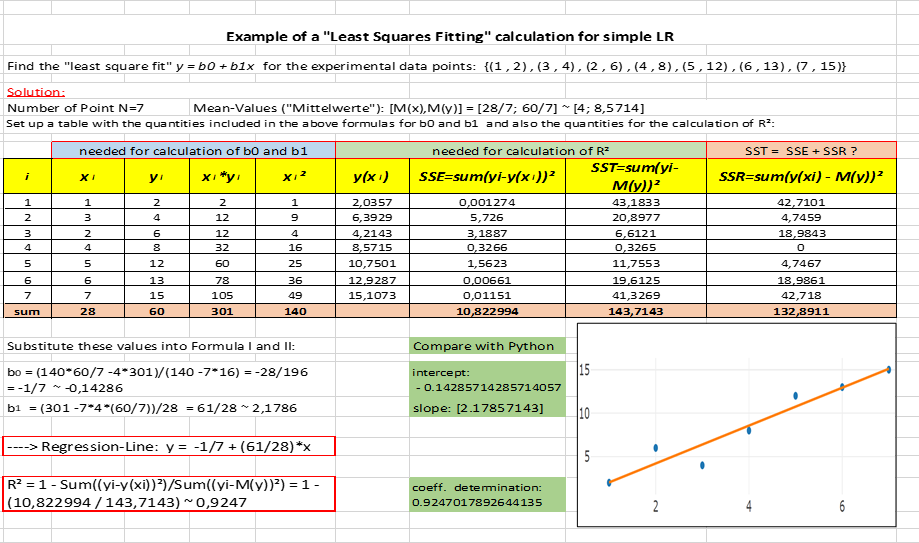
\includegraphics[width=1.25 \textwidth]{Einfaches-sLR_Beispiel}
  \caption{Manuelle Berechnung eines sLR Beispiels}
  \label{fig:einfaches-sLR-Bsp}
\end{figure}
%
\newpage

\subsubsection{Python-Programm zur Berechnung eines sLR Beispiels}
In den folgenden 3 Screenshots eines Jupyter Notebooks sind die expliziten Python Codeblöcke zur Berechnung eines weiteren sLR Beispieles aufgelistet.\\[0.2cm]
\hspace*{0.5cm} \textbf{1. Vorbereitung:}\\
Notwendige Python Bibliotheken zur Verfügung stellen, insbesondere Scikit-learn.
% 
\begin{figure}[htp]
  \centering
  \hspace*{-1.0cm} 
  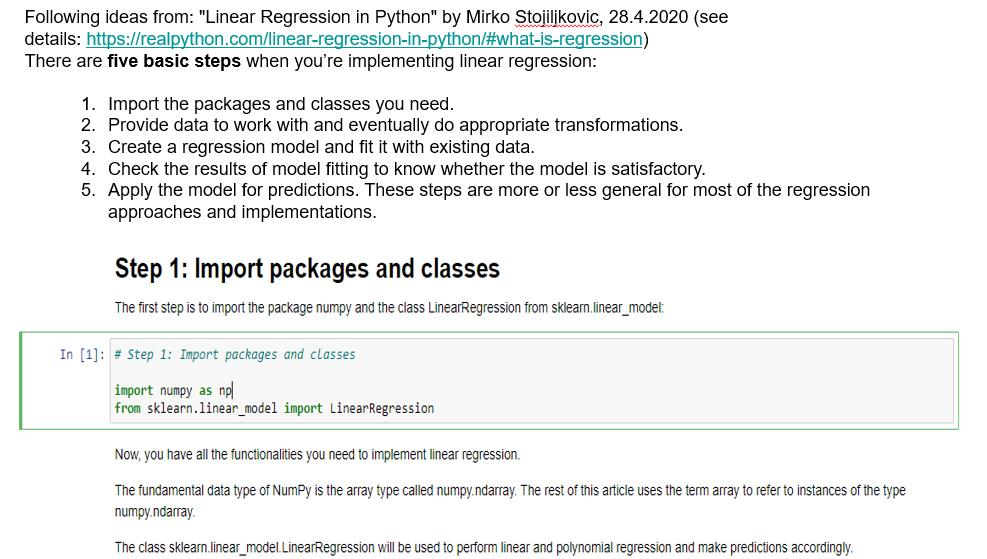
\includegraphics[width=1.25\textwidth]{sLR_Beispiel_Scikit-Learn-01}
  \caption{sLR-Beispiel-Python-1/3}
  \label{fig:sLR-SciKit-Learn01}  
\end{figure}
\\[1.2cm]
\hspace*{0.5cm} \textbf{2. Daten und Modell:}\\
Die sechs Datenpunkte werden definiert (Abm. andere wie im manuellen Beispiel). Das Modell LinearRegression( ) aus der Scikit Bibliothek wird aktiviert. 
\begin{figure}[htp]
  \centering
  \hspace*{-1.0cm} 
  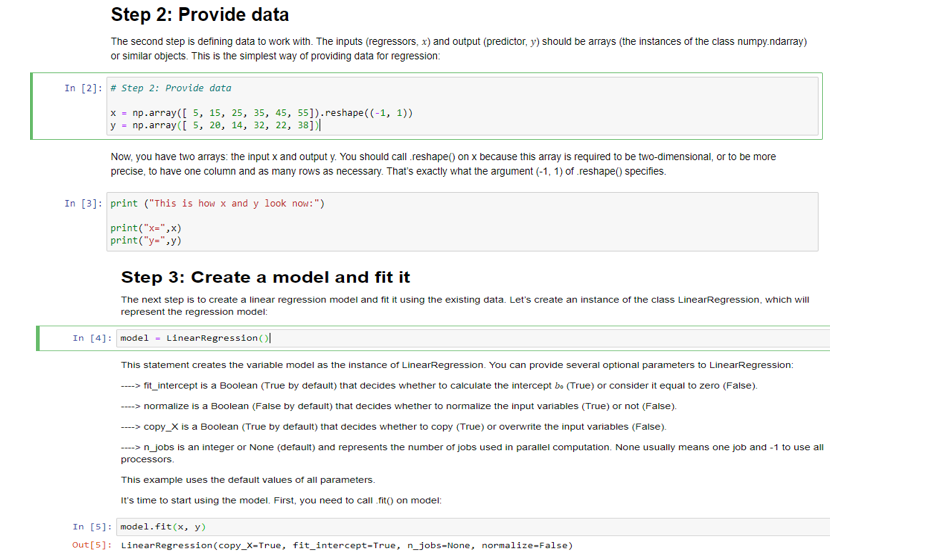
\includegraphics[width=1.4\textwidth]{sLR_Beispiel_Scikit-Learn-02}
  \caption{sLR-Beispiel-Python-2/3}
  \label{fig:sLR-SciKit-Learn02}
\end{figure}
%
\\[1.2cm]
\hspace*{0.5cm} \textbf{3. Ausgabe der Ergebnisse + Datenpunkte:}\\
Bestimmungsgrat $R^2$ und Achsenabschnitt $a$ und Steigung $b$ der Regressiosgeraden werden ausgegeben. Für die sechs Datenpunkte werden auch die Werte $ y(x_i)$ berechnet. 
\begin{figure}[htp]
  \centering
  \hspace*{-0.8cm} 
  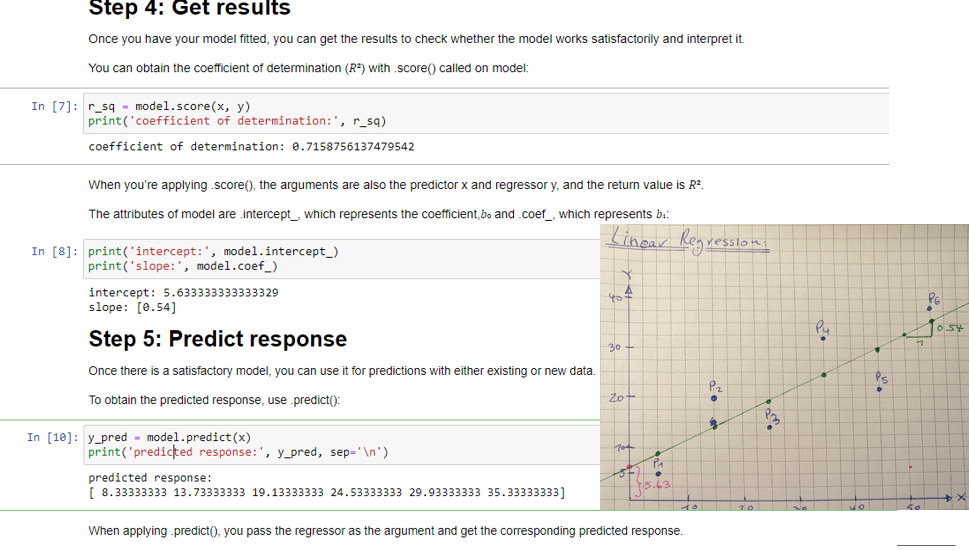
\includegraphics[width=1.2\textwidth]{sLR_Beispiel_Scikit-Learn-03}
  \caption{sLR-Beispiel-Python-3/3}
  \label{fig:sLR-SciKit-Learn02}
\end{figure}
\newpage

\subsection{multiple Lineare Regression mLR(k=2) Beispiele )}

\subsubsection{Manuelle Berechnungen zu einem mLR(k=2) Beispiel}
%
Bei der manuellen Berechnung für einfache Beispiele mit wenigen  Trainingspunkten entwickeln wir einen Excel-Tabelle, wo wir die wichtigsten Parameter/Komponenten für die Berechnung von der optimalen mLR(k=2)-Ebene und dem Bestimmungsgrad $adj.R^2$ per Tabellen-Kalkulation bestimmen lassen.\\

\textbf{1. Berechne opt. Regressionsgerade:}\\[0.2cm]   
Nach (Th-5.4): Sei $ \quad det = \sum{\widetilde{x_i}^2} \cdot \sum{\widetilde{y_i}^2}  -  (\sum{\widetilde{x_i} \cdot \widetilde{y_i}})^2 \quad $ \\
Für den Achsenabschnitt $a$ und die Steigungen $b$ und $c$ einer optimalen mLR(k=2)- Ebene $\quad  z = a +  b \cdot x + c \cdot y \quad $  
gelten folgende Formeln:\\[0.4cm]
\begin{large}
$ \quad a = \bar{z} - b \cdot \bar{x} - c \cdot \bar{y} \ \qquad \qquad \qquad\qquad $ \\[0.3cm]
$ \quad b = \frac{1}{det} \cdot \left[  \sum{\widetilde{y_i}^2} \cdot  \sum{(\widetilde{x_i} \cdot \widetilde{z_i})} - \sum{(\widetilde{x_i} \cdot \widetilde{y_i})} \cdot  \sum{(\widetilde{y_i} \cdot \widetilde{z_i})}          \right] $    \\[0.3cm]                                
$ \quad c = \frac{1}{det} \cdot \left[ \sum{\widetilde{x_i}^2} \cdot  \sum{(\widetilde{y_i} \cdot \widetilde{z_i})} - \sum{(\widetilde{x_i} \cdot \widetilde{y_i})} \cdot  \sum{( \widetilde{x_i} \cdot \widetilde{z_i})}          \right] $ \\[0.5cm]
\end{large}
Also brauchen wir: {\color{blue}{$ n, \quad \bar{x}, \bar{y}, \bar{z}, \quad \sum {\widetilde{x_i}^2}, \sum {\widetilde{y_i}^2}, \quad  \sum {(\widetilde{x_i} \cdot \widetilde{y_i})},  \sum {(\widetilde{x_i} \cdot \widetilde{z_i})}, \sum {(\widetilde{y_i} \cdot \widetilde{z_i})}$}}
\\[0.2cm]
Alle diese Werte werden nun in die Excel-Tabelle eingetragen. Siehe die blauen Felder im nächsten Bild.\\[0.1cm]

\textbf{2. Berechne $adj.R^2$:}\\[0.2cm]
Nachdem die opt. Regressionsebene $z(x,y)$ berechnet ist, lassen sich auch die  Werte SSE und SST berechnen. Siehe grünen Felder im nächsten Bild:\\
\\[0.5cm]

\begin{figure}[htp]
  \centering
  \hspace*{-0.8cm} 
  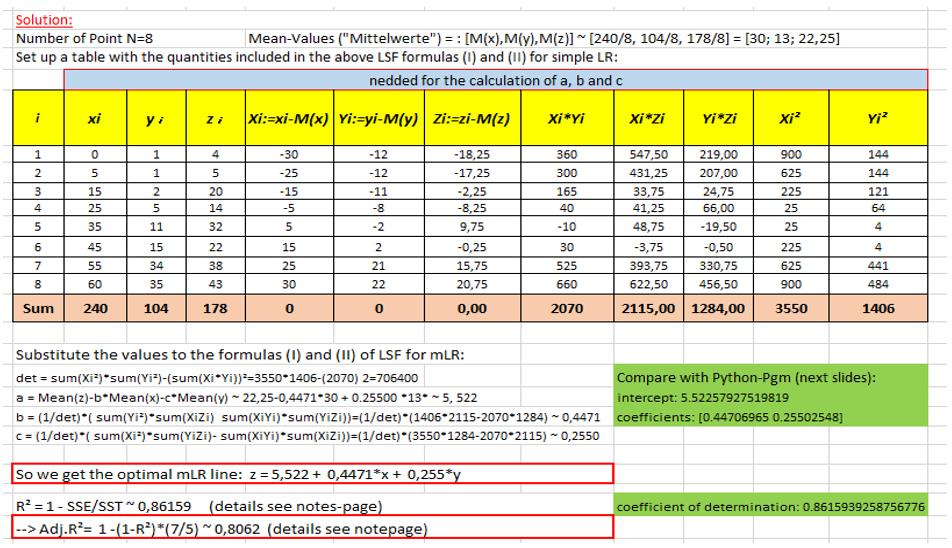
\includegraphics[width=1.2\textwidth]{Einfaches-mLR(k=2)_Beispiel}\\
  \caption{Manuelle Berechnung mLR(k=2)}
  \label{fig:mLR(k=2)-Beispiel}
\end{figure}
\newpage


\subsubsection{Python-Programm zur Berechnung eines mLR(k=2) Beispiels}

{\color{red}
{***** Weitere Kapitel Texte und Beispiele einfügen, siehe Vorlesung *****}}


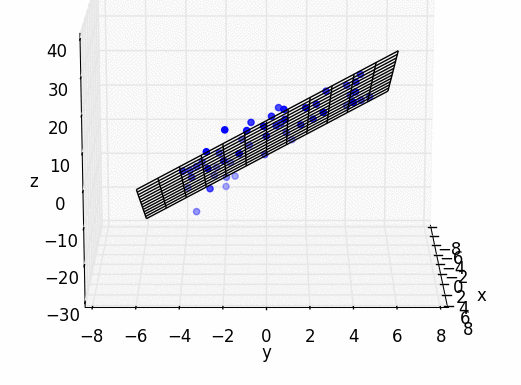
\includegraphics{ML5-MovingPicture_mLR}\\
%
Ein bewegtes Bild davon liegt in der Referenz [HVö-GitML20]: 
{\url{https://github.com/HVoellinger/Lecture-Notes-to-ML-WS2020/blob/master/ML5-QYuIc.gif}}

\subsection{Übungen zum Kapitel 5}
 
Diese Übungen waren teilweise Bestandteil der Vorlesung "Einführung in Maschinelles  Lernen (ML)" im WS 2020 an der DHBW Stuttgart.

\subsubsection{Übung 5.1 - Zwischenergebnis bei (Th-5.3)}

Zeige die im Theorem (Th-5.3) noch nicht bewiesene Behauptung (*):\\ [0.2cm]
(*) $ \qquad 0 = \sum_{i=1}^{n} (y_i - f_i)(f_i - \bar{y})$ für optimale sLR Geraden. 

\subsubsection{Übung 5.2 - Vermutung (V-5.1)}
Beweisen Sie oder Widerlegen Sie folgende \textbf{Vermutung (V-5.1)}:\\[0.2cm]
Aus der Bedingung $ SST = SSE + SSR $ folgt für eine sLR-Gerade, dass diese auch optimal ist in unserer Definition (d.h. R² = maximal).\\

\subsubsection{Übung 5.3 - Zwischenergebnis bei (Th-5.4)}
%\exercise
Zeige die im Theorem (Th-5.4) noch nicht bewiesene Behauptung:\\ 
\hspace*{4.5cm} $ \nabla g(\mathbf{x}) = A^\top \cdot \mathbf{b}$

\subsubsection{Übung 5.4 - Manuelles sLR Beispiel}
Führen Sei die Schritte analog der Vorlesung zur manuellen Befüllung der Excel-Tabelle zur Bestimmung der optimalen sLR-Gerade durch. Prüfen Sie da Ergebnis mit einem kleinen Python Programm. Plotten Sie die optimale sLR-Gerade mit den Ausgangsdatenpunkten. Stimmt das Bild mit Ihrer Erwartungshaltung überein (Datenpunkt 6 und 7)?

\subsubsection{Übung 5.5 - Manuelles mLR(k=2) Beispiel}
Führen Sei die Schritte analog der Vorlesung zur manuellen Befüllung der Excel-Tabelle zur Bestimmung der optimalen mLR-Ebene durch. Prüfen Sie da Ergebnis mit einem kleinen Python Programm. Plotten Sie die opt. mLR-Ebene mit den Ausgangsdatenpunkten. Stimmt das Bild mit Ihrer Erwartungshaltung überein?

\subsubsection{Übung 5.6 - sLR Beispiel "Studentisches Examen"}
%								
\textbf{1. Teil:} Finde eine "least square fit" gerade  y = a + b*x für y:=erreichte Punktzahl (Score) des Examens [pt.]” abhängig vom Parameter: x:="Aufwand der Examens Vorbereitung in Std.[h]". Daten der Trainings-Sets TS  = $ \lbrace (exam vorb.[h]; score[pt.])\rbrace \\
= \lbrace(7;41 ),(3;27), (5;35), (3;26), (8;48), (7;45), (10;46), (3;27), (5;29), (3;19)\rbrace $ \\
Baue das Modell sLR(x,y). Vergleiche und prüfe das Ergebnis mit einem Python-Programm.\\[0.2cm]
\textbf{2. Teil:} Wiederhole obige Aufgabe mit zehn anderen Eingabewerten: \\
 $ \lbrace (homework[h]; score[pt.])\\
= {(5; 41), (4; 27), (5; 35), (3; 26), (9; 48), (8; 45), (10; 46), (5; 27), (3; 29), (3; 19)}\rbrace $\\[0.2cm]
\textbf{Zusatzaufgaben:} Beantworte die folgenden Fragen:\\ 
Q1: Wie viele Punkte würde ein Student ohne Examens Vorbereitung erreichen? Ist dies realistisch (Hinweis: Sinnhaftigkeit von "Bias")?\\
Q1': Wie viele Punkte würde ein Student ohne Hausaufgabe/Homework Aufwand erreichen? Ist dies realistisch (Hinweis: Sinnhaftigkeit von "Bias")?\\
Q2: Wie viele Punkte würde ein Student mit 10 Stunden für Examens Vorbereitung  erreichen? \\ 
Q2': Wie viele Punkte würde ein Student mit 10 Stunden Homework erreichen? \\ 
Q3: Wie viel Aufwand Examens Vorbereitung ist notwendig um genug Punkte (=25) zum Bestehen des Examens?\\
Q3': Wie viel Aufwand Homework ist notwendig um genug Punkte (=25) zum Bestehen des Examens?\\
Q4: Welche Aufwandsart ist aufgrund unserer Trainingsdaten effektiver?\\ 

\subsubsection{Übung 5.7 - mLR(k=2) Beispiel "Studentisches Examen"}
%
Berechne das  mLR(k=2)-Modell studentische Examens-Ergebnisse mit zwei 2 unabhängigen Parametern (Vergleiche auch Übung 5.6):\\  
Finde eine "least square fit" Ebene  z = a + b*x + c*y für z:=erreichte Punktzahl (Score) des Examens [pt.]” abhängig von den zwei Parametern: x:="Aufwand der Examens Vorbereitung in Std.[h]" and y:=Aufwand für Hausaufgaben in Std.[h]“.\\[0.2cm]
Daten der Trainings-Sets $TS$: \\
= $ \lbrace (x, y; z) | (exam vorb.[h], homework[h]; score[pt.])\rbrace = \lbrace(7,5;41 ),(3,4;27), \\
(5,5;35), (3,3;26), (8,9;48), (7,8;45), (10,10;46), (3,5;27), (5,3;29), (3,3;19)\rbrace $ \\[0.2cm]
Baue das Modell mLR(x,y;z). Vergleiche und prüfe das Ergebnis mit einem Python-Programm.\\[0.2cm]
\textbf{Zusatz: Beantworte die folgenden Fragen:}\\ 
Q1: Wie viele Punkte würde ein Student ohne Examens Vorbereitung und ohne Hausaufgabe Aufwand erreichen? \\
Q2: Wie viele Punkte würde ein Student mit 10 Stunden für Examens Vorbereitung und auch mit 10 Std. Hausaufgabe Aufwand erreichen? \\ 
Q3: Wie viel Aufwand für Examensvorbereitung ist notwendig um genug Punkte (=25) zum Bestehen des Examens? Wie gross ist der Aufwand bei Homework?\\[0.2cm]
\textbf{Zusätzliche Frage/Anmerkung:} Unsere Berechnung nutzt beide Variablen zur Berechnung. Was ist der Unterschied zum sLR-Model Resultat? Vergleiche $adj.R^2$ (wie hier genutzt) zu den zwei $R^2$- Lösungen von Übung 5.6.\\
%
\subsubsection{Übung 5.8 - "Beweis zu Korollar (K-5.5)"}
%
Beweise die Aussage von Korollar (K-5.5) und lerne dabei die "Allgemeinen Berechnungen zu LSF-Verfahren" dadurch kennen. Beachte die Hinweise. 
%
\subsubsection{Übung 5.9 - "Beweis zur Anmerkung (A-5.2)-Fall (k=1)"}
%
Beweise die Aussage von Anmerkung (A-5.2) im Fall K=1 und lerne dabei die "Allgemeinen Berechnungen zum LSF-Verfahren (ohne Bias-Trick)" besser kennen.\\
Beachte die Hinweise im Skript. Nutze die Ergebnisse des Beispieles der Berechnung der inversen Matrix zu einer symmetrischen (2x2)-Matrix (Unterkapitel (5.4.1)).
%
\subsubsection{Übung 5.10 - "Beweis zur Anmerkung (A-5.2) Fall (k=2)"}
%
Beweise die Aussage von Anmerkung (A-5.4) im Fall k=2 und lerne dabei die "Allgemeinen Berechnungen zum LSF-Verfahren (ohne Bias-Trick)" besser kennen. \\ Beachte die Hinweise im Skript. Nutze die Ergebnisse des Beispieles der Berechnung der inversen Matrix\index{Inverse} zu einer symmetrischen (3x3)-Matrix (Unterkapitel (5.4.1)).

\subsubsection{Übung 5.1 - "Python-Pgm zu sLR-Verfahren(Iowa Housing Prices)"}
%
Erzeuge ein Python Pgm. (Jupyter Notebook) für eine sLR-Verfahren mit den Daten des Beispiels "Iowa Housing Prices”. Nutze die Informationen aus dem Video:\\
\url{https://www.youtube.com/watch?v=Mcs2x5-7bc0}\\ 

\newpage

\section{Text-Klassifikation via Naive-Bayes Verfahren \\}


Wir zeigen hier Text-Klassifikation mit dem \textbf{Naive Bayes- Klassifikator} ("Bayes Learning" via "naïve Bayes Classifier"). Grundlage ist das Bayes-Theorem ("Bayes Rule"), welches sich mit bedingten Wahrscheinlichkeiten befasst.\\
Die {\color{blue}{Naive-Bayes-Textklassifikation}} \index{Naive-Bayes-Textklassifikation} ist eine Methode des maschinellen Lernens, die auf dem Naive-Bayes-Theorem basiert und häufig zur Kategorisierung von Textdaten verwendet wird. Sie ist besonders nützlich für Anwendungen wie Spam-Erkennung, Sentiment-Analyse, Themenklassifikation und mehr.\\

Der Ansatz ist "naiv", weil er eine starke Unabhängigkeitsannahme zwischen den Features (Wörtern) macht, was in der Praxis oft nicht der Fall ist.

\subsection{Eine Einführung in den naiven Bayes-Klassifikator}

Hier ist eine grundlegende Erklärung, wie die {\color{blue}{Naive-Bayes-Textklassifikation}} \index{Naive-Bayes-Textklassifikation} funktioniert:\\

\begin{figure}[htb]
  \centering
  \hspace*{-1.5cm} 
  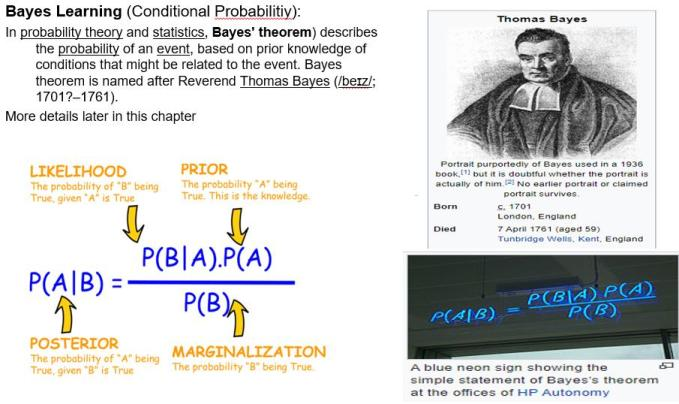
\includegraphics[width=1.2\textwidth]{Naive-Bayes-Learning}
  \caption{Screenshots zum Naive-Bayes-Learning}
\label{fig:NB_Learning}
\end{figure}


\textbf{1. Naive-Bayes-Theorem:}\\
Das Naive-Bayes-Theorem ist eine statistische Formel, die auf dem Satz von Wahrscheinlichkeitsregeln beruht, bekannt als \textbf{Bayes-Theorem}. Es gibt an, wie Wahrscheinlichkeiten nach der Anwendung neuer Informationen aktualisiert werden. Für die Textklassifikation bedeutet dies, dass wir die Wahrscheinlichkeit berechnen, mit der ein Dokument einer bestimmten Klasse (z. B. "Positiv" oder "Negativ") angehört, basierend auf den darin enthaltenen Wörtern.\\
\textbf{2. Feature-Extraktion:}\\
Für jeden Text werden Features (Wörter) extrahiert, die als Eingabe für den Naive-Bayes-Klassifikator dienen. In der Regel werden diese Wörter als "Bag of Words" betrachtet, d. h. die Reihenfolge der Wörter im Text wird ignoriert.\\
\textbf{3. Berechnung der Wahrscheinlichkeiten:}\\
Für jede Klasse wird die Wahrscheinlichkeit berechnet, dass ein gegebenes Dokument dieser Klasse angehört. Dies erfolgt, indem die Wahrscheinlichkeiten für jedes im Dokument vorkommende Wort (Feature) multipliziert werden. Die Wahrscheinlichkeiten werden aus Trainingsdaten abgeleitet.\\
\textbf{4. Klassifikation:}\\
Das Dokument wird der Klasse zugeordnet, für die die berechnete Wahrscheinlichkeit am höchsten ist. Dies wird oft durch den Satz von Klassenlabels erreicht, die im Trainingsprozess erlernt wurden.\\
\textbf{5. Laplace-Glättung:}\\
Ein Problem bei der Verwendung von Wahrscheinlichkeiten auf der Grundlage von Trainingsdaten ist, dass einige Wörter möglicherweise in bestimmten Klassen überhaupt nicht vorkommen. Dies könnte dazu führen, dass die berechnete Wahrscheinlichkeit null wird und das Modell nicht in der Lage ist, Vorhersagen für diese Klasse zu treffen. Um dieses Problem zu mildern, wird oft die Laplace-Glättung verwendet, um die Wahrscheinlichkeiten leicht zu verschieben.\\[0.2cm]

\textbf{Zusammenfassung:}\\
Naive-Bayes-Klassifikatoren sind einfach zu implementieren, schnell und können auch bei begrenzten Trainingsdaten gut funktionieren. Allerdings kann die starke Unabhängigkeitsannahme zwischen den Features in einigen Fällen zu weniger genauen Vorhersagen führen, insbesondere wenn es komplexe Abhängigkeiten zwischen den Wörtern gibt. Dennoch ist die Naive-Bayes-Textklassifikation eine nützliche Methode, um eine erste Annäherung an die Klassifikation von Textdaten zu erhalten.\\

\subsection{Mathematische Grundlagen bei Textklassifikatoren}
{\color{red}{*******************************************************************\\ 
ab hier bis Ende der section sind die Folien der Vorlesung ML  zu nutzen und diese sind in Latex umzusetzen\\
********************************************************************\\}}

\
\subsubsection{Bayes-Learning für Texte}

\begin{center} 
\hspace*{-1.5cm} 
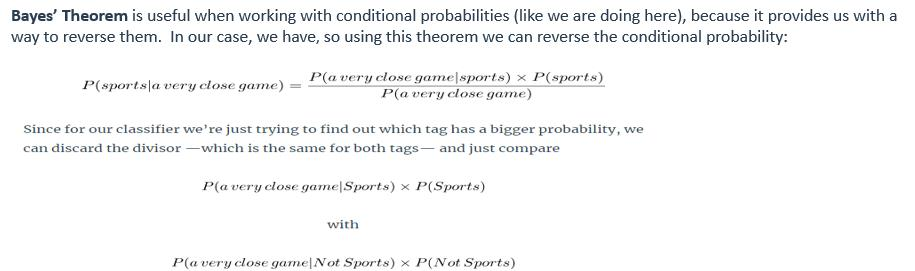
\includegraphics[width=1.2\textwidth]{Bayes-Rule01}
\end{center}

\subsubsection{"Laplace Glättung"}

\begin{center} 
\hspace*{-1.5cm} 
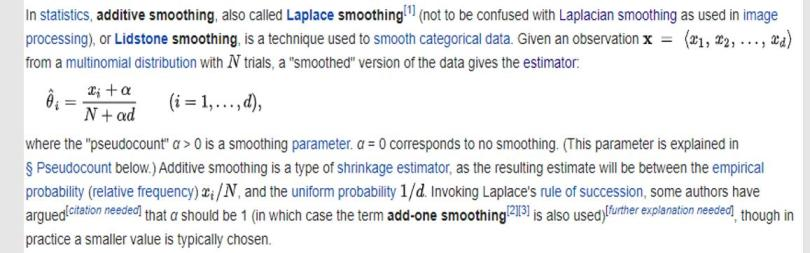
\includegraphics[width=1.2\textwidth]{Bayes-Rule02}
\end{center}

\subsection{Konkrete Anwendung des naiven Bayes-Klassifikator}

\begin{center}
\hspace*{-1.cm}   
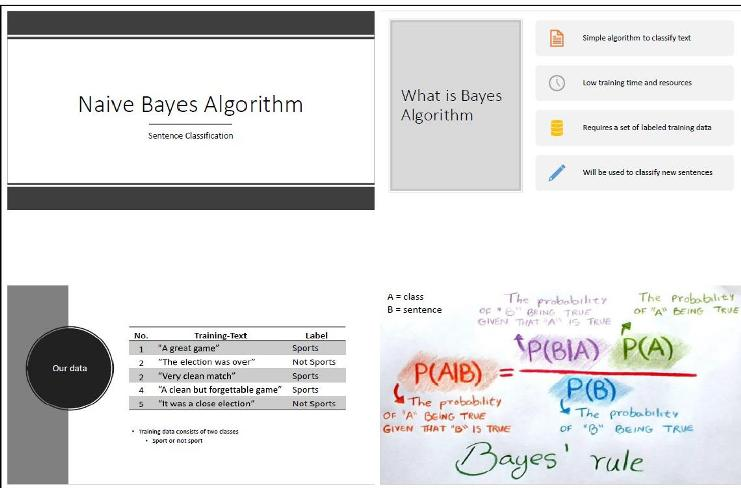
\includegraphics[width=1.2\textwidth]{Bayes-Text-Classification01}
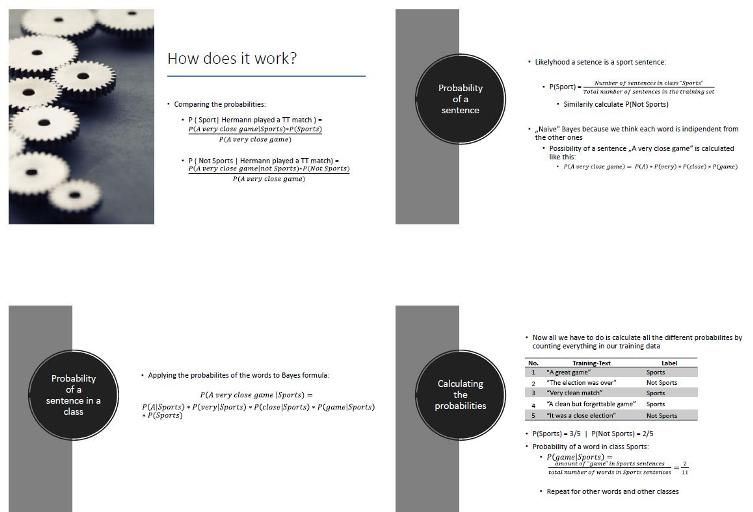
\includegraphics[width=1.1\textwidth]{Bayes-Text-Classification02}
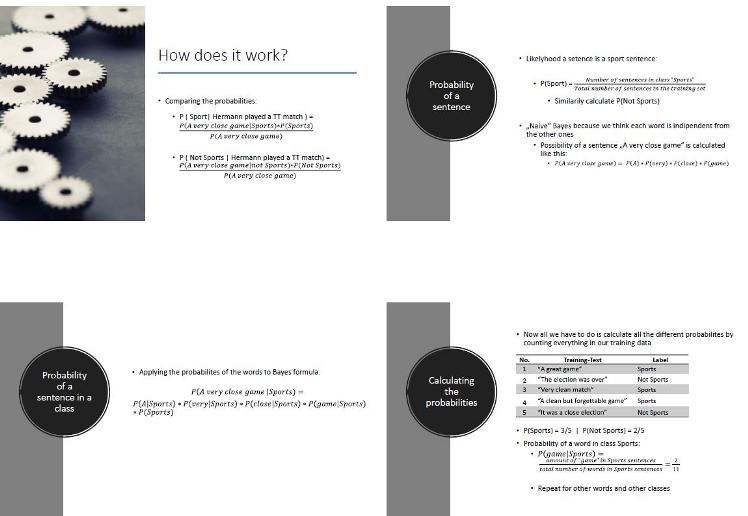
\includegraphics[width=1.1\textwidth]{Bayes-Text-Classification03}
\end{center}

\begin{center}  
\hspace*{-2.8cm} 
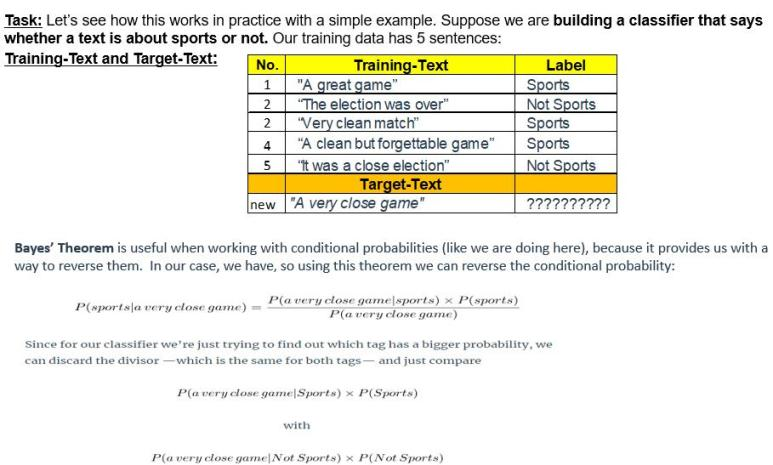
\includegraphics{Bayes-Beispiel01}
\end{center}

\begin{center}  
\hspace*{-2.5cm} 
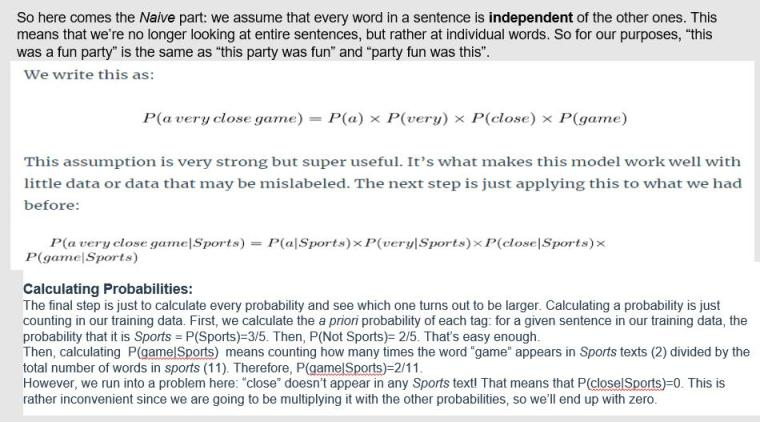
\includegraphics{Bayes-Beispiel02}
\end{center}\begin{center}  

\hspace*{-1.8cm} 
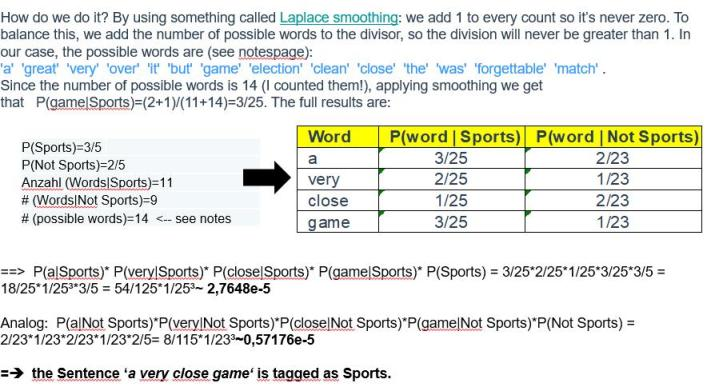
\includegraphics{Bayes-Beispiel03}
\end{center}

\newpage

\subsection{Übungen zum Kapitel 6}

{\color{red}{*******************************************************************\\ ab hier bis Ende der Übungen sind die Folien der Vorlesung ML  zu nutzen und diese sind in Latex umzusetzen\\
********************************************************************\\}}
.....\\



\subsubsection{Übung 6.1 - Bsp. einer Bayes-Texklassifikation}

Analog dem Beispiel aus obigen Kapitel soll die Bayes- Textklassifikation für einen weiteren Zielsatz mit den gleichen \textbf{"gelabelten" Trainingsdaten} durchgeführt werden. Wir suchen jetzt eine Klassifikation für den Zielsatz \textbf{"Hermann plays a TT match"}:\\   

\begin{center} 
\includegraphics[width=0.8\textwidth]{Bayes-Learning-Übungen}
\end{center}

\textbf{Zusatzfrage:} Wie verändert sich das Ergebnis wenn ich als Zielsatz: \textbf{"Hermann plays a very clean game"} eingebe? 


\subsubsection{Übung 6.2 - Bayes-Textklassifikation in Python}

Definiere einen Algorithmus in Python (benutze Jupyter Notebook) um obige Berechnung zu automatisieren. Tipp: Vergleich analoge Beispiele in \textbf{[HVö-GitML20]} - \url{https://github.com/HVoellinger/Lecture-Notes-to-ML-WS2020}\\

\subsubsection{Übung 6.3}:
*** Weitere Kapitel Texte *** 

\newpage

\section{Verfahren der Support Vector Machines (SVM)\\} 
%
*** Referenzen: [Wiki-SVM]; [SVM-Def] und  [TK + SVM]*****\\
%
Wichtig zum Verständnis von {\color{blue}{Support Vector Machines (SVM)}}\index{Support Vector Machines} ist die Beschreibung einiger mathematischen Grundlagen der SVM.\\
Diese sind in der Tat traditionelle Lineare Algebra und keine "Rocket Science". Es geht bei diesem Klassifikationsproblem darum optimale Hyperebenen zu finden die die Klassen "gut" trennen.
Dies kann man etwa auch gut am Beispiel von Text-Klassifikationen sehen. Text-Klassifikatiion hat sehr viel mit SVM zu tun. Vergleichen Sie dazu die Beispiele die in der Referenz [TK + SVM] zu sehen sind.
\subsection{Grundlegende mathematische Funktionsweise}
Das Hauptziel der SVM besteht darin, eine optimale Trennung (Klassifikation) zwischen zwei Klassen von Datenpunkten in einem mehrdimensionalen Raum zu finden. Die SVM sucht eine Hyperebene, die die beiden Klassen maximal voneinander trennt, wobei der Abstand zwischen der Hyperebene und den nächsten Datenpunkten (den sogenannten Support-Vektoren) maximiert wird.
\\
\textbf{Mathematisch Schreibweise:}
\\Angenommen, wir haben eine Menge von Trainingsdatenpunkten: ${(x_1, y_1), (x_2, y_2),... , (x_n, y_n)}$, wobei $x_i \in \mathbb{R}^n$ der Eingabevektor und $y_i$ als Klasse von Datenpunkten nur die Werte +1 oder -1 annehmen kann.\\
Für eine lineare SVM ist die mathematische Darstellung der Hyperebene dann gegeben durch:
\begin{center}
\begin{large} \textbf{$w \cdot x + b = 0$} \end{large} 
\end{center}
Hier ist "$w$" der Gewichtsvektor, der senkrecht zur Hyperebene zeigt und die Richtung der Trennung bestimmt. "$b$" ist der Bias (auch Verschiebungsparameter genannt), der die Verschiebung der Hyperebene entlang der "$w$"-Achse steuert. Es gelten dabei die folgenden \textbf{matematischen Bedingungen}\\
\textbf{1. Lineare Trennbarkeit:}\\
Die {\color{blue}{SVM}} \index{Support Vector Machines} hat bestimmte Trennbedingungen, die während des Trainingsprozesses erfüllt werden sollen:
Die Punkte jeder Klasse müssen auf unterschiedlichen Seiten der Hyperebene liegen.\\
Mathematisch ausgedrückt gilt für positive Beispiele ($y_i = 1$): $w \cdot x_i + b \geq 1$\\
und für negative Beispiele ($y_i = -1$): $w \cdot x_i + b \leq -1$\\
Der Abstand (Margin) zwischen den nächsten Datenpunkten (Support-Vektoren) und der Hyperebene muss maximal sein. Der Abstand zwischen zwei parallelen Hyperebenen, die die Support-Vektoren berühren, wird als Margin bezeichnet.\\
\textbf{2. Optimierung:}\\Das Ziel der SVM ist es, den Margin zu maximieren, indem die Länge des Gewichtsvektors "$w$" minimiert wird. Das führt zu einem quadratischen Optimierungsproblem. In der linearen SVM lautet das Optimierungsproblem:
\begin{center}
\begin{large} \textbf{Minimiere $||w||^2$} \end{large} \\
Unter den Bedingungen: $y_i \cdot (w \cdot x_i + b) \geq 1$ für alle Datenpunkte ${(x_i,y_i)}$
\end{center}
\textbf{3. Kernel-Trick:}\\
In Fällen, in denen die Daten nicht linear separierbar sind, kann der sogenannte  {\color{blue}{Kernel-Trick}} \index{Kernel-Trick} angewendet werden. Der Kernel-Trick ermöglicht es, die Daten in einen höherdimensionalen Raum zu transformieren, in dem sie linear separierbar werden. Beliebte Kernel-Funktionen sind beispielsweise der lineare Kernel, der polynomiale Kernel und der RBF (Radial Basis Function) Kernel.\\

\textbf{Anmerkung: Wie kommt es zu dem Namen "Kernel-Trick"?}\\
Der Name "Kernel" kommt daher, dass in der mathematischen Darstellung der SVM die Funktion, die die Datenpunkte in den höherdimensionalen Raum transformiert, als Kernel-Funktion bezeichnet wird.\\

Dies sind die grundlegenden mathematischen Grundlagen der Support Vector Machine. SVM ist eine äußerst flexible und leistungsfähige Methode, die in vielen Anwendungen erfolgreich eingesetzt wird.\\

*** Weitere Kapitel Texte *** 

\subsection{Funktionsweise im Detail}

Ausgangsbasis für den Bau einer {\color{blue}{Support Vector Machine}} \index{Support Vector Machines}ist eine Menge von Trainingsobjekten, für die jeweils bekannt ist, welcher Klasse sie zugehören. Jedes Objekt wird durch einen Vektor in einem Vektorraum repräsentiert. Aufgabe der Support Vector Machine ist es, in diesen Raum eine Hyperebene einzupassen, die als Trennfläche fungiert und die Trainingsobjekte in zwei Klassen teilt. Der Abstand derjenigen Vektoren, die der Hyperebene am nächsten liegen, wird dabei maximiert. Dieser breite, leere Rand soll später dafür sorgen, dass auch Objekte, die nicht genau den Trainingsobjekten entsprechen, möglichst zuverlässig klassifiziert werden.
\begin{center} 
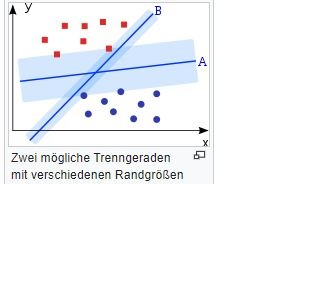
\includegraphics{SVM-Konzept} 
\end{center}
Beim Einsetzen der Hyperebene ist es nicht notwendig, alle Trainingsvektoren zu beachten. Vektoren, die weiter von der Hyperebene entfernt liegen und gewissermaßen hinter einer Front anderer Vektoren "versteckt" sind, beeinflussen Lage und Position der Trennebene nicht. Die Hyperebene ist nur von den ihr am nächsten liegenden Vektoren abhängig – und auch nur diese werden benötigt, um die Ebene mathematisch exakt zu beschreiben. Diese nächstliegenden Vektoren werden nach ihrer Funktion Stützvektoren (engl. support vectors) genannt und verhalfen den Support Vector Machines zu ihrem Namen.

\subsubsection{Lineare Trennbarkeit}

Eine Hyperebene kann nicht "verbogen" werden, sodass eine saubere Trennung mit einer Hyperebene nur dann möglich ist, wenn die Objekte linear trennbar sind.\\ 
\begin{center}  
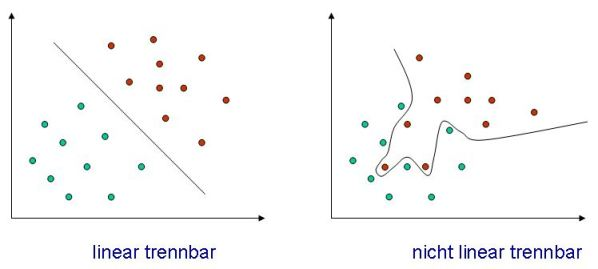
\includegraphics{Trennbarkeit}
\end{center}
Diese Bedingung ist für reale Trainingsobjektmengen im Allgemeinen nicht erfüllt. Support Vector Machines verwenden im Fall nichtlinear trennbarer Daten den {\color{blue}{Kernel-Trick}}\index{Kernel-Trick}, um eine nichtlineare Klassengrenze einzuziehen.\\

\subsubsection{Kernel-Trick} 
Die Idee dahinter ist, den Vektorraum in einen höherdimensionalen Raum zu überführen, wo die Objekte linear trennbar sind und dort eine Hyperebene zu definieren. In einem Raum mit genügend hoher Dimensionsanzahl – im Zweifelsfall unendlich – wird auch die verschachtelteste Vektormenge linear trennbar. In diesem höherdimensionalen Raum wird nun die trennende Hyperebene bestimmt. Bei der Rücktransformation in den niedrigerdimensionalen Raum wird die lineare Hyperebene zu einer nichtlinearen, unter Umständen sogar nicht zusammenhängenden Hyperfläche, welche die Trainingsvektoren sauber in zwei Klassen trennt.\\
Bei diesem Vorgang stellen sich zwei Probleme: Die Hochtransformation ist enorm rechenintensiv und die Darstellung der Trennfläche im niedrigdimensionalen Raum im Allgemeinen unwahrscheinlich komplex und damit praktisch unbrauchbar. An dieser Stelle setzt der \textbf{Kernel-Trick} an. \\ Verwendet man zur Beschreibung der Trennfläche geeignete Kernelfunktionen, die im Hochdimensionalen die Hyperebene beschreiben und trotzdem im Niedrigdimensionalen "gutartig" bleiben, so ist es möglich, die Hin- und Rücktransformation umzusetzen, ohne sie tatsächlich rechnerisch ausführen zu müssen. Auch hier genügt ein Teil der Vektoren, nämlich wiederum die Stützvektoren, um die Klassengrenze vollständig zu beschreiben.\\
Sowohl lineare als auch nichtlineare Support Vector Machines lassen sich durch zusätzliche \textbf{Schlupfvariablen} flexibler gestalten. Die Schlupfvariablen erlauben es dem Klassifikator, einzelne Objekte falsch zu klassifizieren, "bestrafen" aber gleichzeitig jede derartige Fehleinordnung. Auf diese Weise wird zum einen Überanpassung vermieden, zum anderen wird die benötigte Anzahl an Stützvektoren gesenkt.

\subsection{Anschauliches 2-dim. Beispiel für Kernel-Trick}

Stellen wir uns ein einfaches und anschauliches Beispiel in $\mathbb{R}^2$ vor, bei dem die Datenpunkte im ursprünglichen Raum $(x_1,x_2)$ nicht linear trennbar sind.\\ 
Gesucht ist dann eine Abbildung $\Phi:\mathbb{R}^2 \rightarrow\mathbb{R}^3$, so das die Datenpunkte im höherdimensionalen Raum $(x,y,z)\in  \mathbb{R}^3$ linear trennbar sind.\\ 
Der Kernel-Trick ermöglicht es der SVM, die Entscheidungsgrenze in diesem höherdimensionalen Raum zu finden, ohne die zusätzlichen Merkmale $z$ tatsächlich berechnen zu müssen:\\ 
\subsubsection{Definition des Kernel-Trick Beispieles}
Gegeben sind die folgenden Datenpunkte: {\color{red}{Klasse +1: A(1,1), B(-1,1)}} und {\color{blue}{Klasse -1: C(2,1), D(1,-2) und E(-2,1)}}.\\
In diesem Beispiel sind die Datenpunkte nicht linear trennbar (siehe auch nachfolgende Skizze). Es gibt keine gerade Linie, die die Punkte der {\color{red}{Klasse +1}} von den Punkten der {\color{blue}{Klasse -1}} perfekt trennen kann.\\
Jetzt wenden wir den Kernel-Trick an, um die Daten in $\mathbb{R}^3$ zu transformieren. Hier verwenden wir den polynomiellen Kernel über die folgende Transformation an: 
\begin{center}
 $\Phi:\mathbb{R}^2 \rightarrow\mathbb{R}^3$ definiert durch  $\Phi(x_1,x_2) = (x_1,x_2, x_1^2 + x_2^2)$. 
\end{center} 
Die transformierten Punkte A' = $\Phi(A)$ ....E' = $\Phi(A)$ werden dann berechnet als: {\color{red}{Klasse +1: A'(1,1,2), B'(-1,1,2)}} und {\color{blue}{Klasse -1: C'(2,1,5), D'(1,-2,5) und E'(-2,1,5)}}. Die roten Punkte liegen dabei alle auf der Höhe z=2 und die blauen Punkte auf z=5. Siehe dazu den folgenden Python Plot:\\[0.2cm]

\newpage

\begin{figure}[ht]
  \centering
  \hspace*{-0.5cm} 
  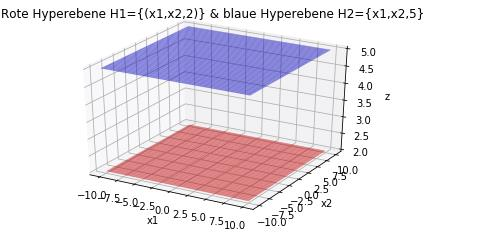
\includegraphics[width=0.9\textwidth]{Kernel-Hyperebene-Bild}
  \caption{Hyperebenen zum Kernel-Trick Beispiel}
  \label{fig:SVM_Ebenen}
\end{figure}
%
Ein bewegtes Bild davon liegt in der Referenz \textbf{[HVö-GitML20]:} \url{https://github.com/HVoellinger/Mathematische-Grundlagen_von_ML/blob/main/Images/hyperebenen_animation.gif}\\[0.2cm]
%
Wie man leicht aus dem Plot sieht, lassen sich diese Punkte optimal durch eine Hyperebene ${H := \lbrace (x_1,x_2,z)| z=3.5\rbrace}$ trennen. Der Normalenvektor dieser Ebene ist in z-Richtung also $(0,0,1) in \mathbb{R}^3 $. Da alle Punkte A' bis E' den gleichen Abstand 1.5 zu dieser Hyperebene haben, sind diese alle "Stützvektoren im Sinne von SVM (siehe oben). \\ 
Durch eine "Zurücktransformation" erhält man den \textbf{Kreis: $x_1^2+x_2^2=3,5$ } mit den Radius $r = \sqrt[2]{3,5} \approx 1.871 $  Damit ergibt sich die visuelle Darstellung der Klassifikation-Trennlinie als Kreislinie. Wir lassen uns diesen Kreis via einem kleinem Python Programm zeichnen:\\[0.2cm]
\begin{figure}[tp]
  \centering
  \hspace*{-0.1cm} 
  \includegraphics[width=1.1\textwidth]{SVM-Kreisbild-Python}
  \caption{Python Code und Kernel-Trick Kreisbild}       
  \label{fig:SVM_Kreis}
\end{figure}
%
\newpage
\subsubsection{Berechnung per Jupyter Notebook}
Wenn es mehr Daten-Punkte gibt (was die Regel ist) müssen wir Algorithmen einsetzen. Die Beispiele werden dann auch entsprechend komplizierter und können nicht mehr manuell berechnet werden. Die Normalvektoren $ (0,0,1)in {R}^3 $ sind sicherlich nicht senkrecht, sondern haben Beiträge in x- und y-Richtung.\\
Ein solches Beispiel soll als Übungsbeispiel in Übung(7.1) gerechnet werden\\[0.3cm]
% 
Um ein einfaches und anschauliches Beispiel für eine Support Vector Machine (SVM) mit einem Kernel-Trick von 2D nach 3D in einem Jupyter Notebook zu erstellen, können Sie den folgenden Python-Code verwenden. Der Code 
verwendet die scikit-learn Bibliothek für die SVM und die matplotlib Bibliothek zum Plotten. Zur Programmierung in Python importieren wir zuerst die erforderlichen Bibliotheken.... Hier das komplette Notebook:\\[0.2cm]
\textbf{\url{https://github.com/HVoellinger/Mathematische-Grundlagen_von_ML/blob/main/Quellen_Math-ML/SVM-Kernel-2D-3D.pdf}}\\
Ein mögliches Ergebnis könnte wie folgt aussehen: \\
\begin{figure}[tp]
  \centering
  \hspace*{-0.1cm} 
  \includegraphics[width=1.\textwidth]{SVM-Kernel(2D-3D)-Beispiel}
  \caption{Kernel-Trick(2D-3D) Beispiel}    
  \label{fig:SVM_2D-3D}
\end{figure}
%
\newpage

\subsection{Übungen zum Kapitel 7}



{\color{red}{*******************************************************************\\ 
ab hier bis Ende der Übungen sind die Folien der Vorlesung ML  zu nutzen und diese sind in Latex umzusetzen\\
********************************************************************\\}}
%
\subsubsection{Übung 7.1 - Einfaches Kernel-Trick(2D nach 3D)- Beispiel}
%
Berechnen Sie analog zum Kapitel (7.3) ein einfaches und anschauliches Beispiel für eine Support Vector Machine (SVM) mit einem Kernel-Trick von 2D nach 3D in einem Jupyter Notebook.\\
Sie nehmen wieder 2 Klassen +1 und -1 mit jetzt 5 Daten-Punkten. Wählen Sie eine passende Transformation von 2D nach 3D.\\
Gegen Sie die SVM-Ebene an mit Ebenen-Gleichung (Normalvektor), Stützvektoren an. Visualisieren Sie die Punkte und Trennlinie in 2D und in 3D \\[0.2cm]\\
\subsubsection{Übung 7.2 - Vergleich Polymonischer Kernel mit RBF Kernel}
%
In dieser Übung erstellen wir einen Datensatz mit Punkten, die konzentrische Kreise bilden, die im ursprünglichen Merkmalsraum nicht linear separierbar sind. Wir verwenden dann zwei SVM-Modelle: eines mit einem Polynomischen Kernel und ein anderes mit einem RBF-Kernel (Radial Basis Function). Der RBF-Kernel wendet effektiv den Kernel-Trick an, indem er die Daten in einen höherdimensionalen Raum transformiert, in dem sie linear trennbar werden. Die Entscheidungsgrenzen und Datenpunkte werden grafisch dargestellt, um den Unterschied zwischen den beiden Kerneln zu verdeutlichen.
Der RBF-Kernel wird in der Praxis häufig verwendet, um nicht linear trennbare Daten zu verarbeiten, und ist eine der wichtigsten Anwendungen des Kernel-Tricks in der SVM.
Hier ein Beispiel Notebook:\\[0.5cm]
\textbf{\url{https://github.com/HVoellinger/Mathematische-Grundlagen_von_ML/blob/main/Quellen_Math-ML/SVM-RBF+Polyn-Kernel.pdf}}\\[0.5cm]


\subsubsection{Übung 7.3 - Python Code zu Hyperebenen}
Schreiben Sie den Python Code zur Generierung der zwei Hyperebenen im 2-dim. Beispiel zum Kernel-Trick. Animieren Sie die Grafik, so dass sie sich dreht. 

\newpage

\section{Neuronale Netzwerk,i.e.Tiefe Neuronale Netzwerke }

\textbf{Neuronale Faltungsnetzwerke} sind eine spezielle Art von künstlichen neuronalen Netzwerken, die hauptsächlich für die Verarbeitung von strukturierten Daten wie Bildern oder anderen Gitterdaten entwickelt wurden. Sie sind besonders effektiv bei der Extraktion von Merkmalen aus solchen Daten, was sie ideal für Aufgaben wie Bilderkennung und Bildklassifikation macht.
\\
Der Name "Faltungsnetzwerke" leitet sich von der \textbf{Faltungsoperation} ab, die in diesen Netzwerken eine wichtige Rolle spielt. Diese Operation ermöglicht es, lokale Merkmale oder Muster in den Eingabedaten zu erkennen, indem sie über die Daten "geschoben" wird. Diese Merkmale werden dann auf höheren Ebenen des Netzwerks kombiniert, um komplexere Muster und Strukturen zu identifizieren.
\\{\color{blue}{Faltungsnetzwerke)}}\index{Faltungsnetzwerke)} sind eine spezielle Art von \textbf {Deep-Learning-Modellen}. Insgesamt bezieht sich "Deep Learning" auf den Einsatz von neuronalen Netzwerken mit mehreren Schichten (daher "tief") für das Lernen von Darstellungen und Mustern in Daten. Faltungsnetztwerke sind nur eine von vielen Architekturen im Bereich des Deep Learning.\\
. Ein DNN besteht neben dem Eingabe- und Ausgabe-Schicht noch aus sehr vielen weiteren "versteckten" Schichten ("Hidden Layers"). Jede Schicht(Layer) enthält eine bestimmte Anzahl von Neuronen oder Aktivierungseinheiten.\\
DNNs haben in den letzten Jahren große Fortschritte erzielt und sind zum Beispiel in der Bilderkennung, Gesichtserkennung, medizinischen Bildverarbeitung und sogar in der natürlichen Sprachverarbeitung (mit Modellen wie den sogenannten "Convolutional Seq2Seq" Modellen) weit verbreitet.\\
\subsection{Anwendung von DNN - "ChatGPT"}
%
{\color{blue}{ChatGPT)}} \index{ChatGPT}ist eine der bekanntesten Anwendungen von DNN's mit erstaunlichen Ergebnissen.
Aber lassen wir ChatGPT mal selbst sprechen und stellen entsprechende Fragen ans Tool:\\
\begin{figure}[tp]
  \centering
  \hspace*{-0.1cm} 
  \includegraphics[width=1.\textwidth]{ChatGPT ist ein tiefes neuronales Netz}
  \caption{ChatGPT ist ein tiefes neuronales Netz} 
  \label{fig:ChatGPt=DNN}
\end{figure}
\begin{figure}[tp]
  \centering
  \hspace*{-0.1cm} 
  \includegraphics[width=1.\textwidth]{ChatGPT nutzen Generative Pretrained Transformer(CPT)}
  \caption{ChatGPT nutzen Generative Pretrained Transformer(CPT)}     
  \label{fig:ChatGPt-Transformer}
\end{figure}
\\[10.2cm] 
***\\ Weitere Kapitel Texte \\
***\\
**** Referenz: [Math for DL] ******** 
\subsection{Mathematische Grundlagen von Faltungsnetzwerken}
%
Die mathematischen Grundlagen des {\color{blue}{Faltungsnetzwerke: Englisch auch oft Convolutional Neural Networks (CNN)genannt }}\index{Convolutional Neural Network (CNN)} beruhen auf Konzepten aus linearen Algebra, partiellen Ableitungen und Faltung (Convolution). Ein CNN ist eine spezielle Art von neuronalem Netzwerk, das häufig in der Bild- und Sprachverarbeitung eingesetzt wird, aufgrund seiner Fähigkeit, räumliche Strukturen in Daten zu erkennen.\\
\subsubsection{Liste der wichtigsten mathematische Methoden}
Hier sind die wichtigen mathematischen Grundlagen eines Convolutional Neural Networks:\\
%
\textbf{1. Lineare Algebra:}\\
CNNs verwenden Matrizenoperationen, um Gewichte und Aktivierungen zu berechnen. Ein typischer Schritt in einem CNN ist die lineare Transformation, bei der Eingabedaten durch eine Gewichtsmatrix multipliziert und ein Bias addiert wird. Dies erzeugt die Aktivierungen der nächsten Schicht.\\
\textbf{2. Faltung (Convolution):}\\
Die Faltung ist ein zentrales Konzept in CNNs. In einem CNN werden Filter (auch Kernel genannt) verwendet, um räumliche Merkmale aus den Eingabedaten zu extrahieren. Die Faltung erfolgt durch das Verschieben des Filters über die Eingabedaten und die Berechnung des Punktprodukts zwischen dem Filter und dem überlappenden Teil der Daten. Das Ergebnis ist ein sogenanntes Aktivierungsmuster oder Feature-Map, das die erkannten Merkmale anzeigt.\\
\textbf{3. Nichtlinearität (Aktivierungsfunktionen):}\\
Nach der Faltung wird in den meisten Schichten des CNN eine Nichtlinearität eingeführt, um die Expressivität des Netzwerks zu erhöhen. Eine Aktivierungsfunktion wie die ReLU (Rectified Linear Unit) wird oft verwendet, um negative Werte zu eliminieren und nichtlineare Verzerrungen in den Daten zu erzeugen.\\
\textbf{4. Pooling:}\\
Pooling ist ein weiterer wichtiger Schritt in CNNs, um die räumliche Dimension der Daten zu reduzieren und die Invarianz gegenüber leichten Translationen zu erreichen. Typischerweise wird Max-Pooling angewendet, bei dem der maximalste Wert aus einem kleinen Ausschnitt der Daten beibehalten wird.\\
\textbf{5. Backpropagation:}\\
Wie bei anderen neuronalen Netzwerken werden CNNs mit dem Backpropagation-Algorithmus trainiert. Backpropagation verwendet die Kettenregel der partiellen Ableitungen, um die Gewichte des Netzwerks so anzupassen, dass der Fehler zwischen den vorhergesagten und tatsächlichen Ausgaben minimiert wird.\\
\textbf{6. Mehrschichtige Struktur:}\\
CNNs bestehen aus mehreren Schichten, darunter Eingabeschicht, Faltungsschichten, Aktivierungsschichten, Pooling-Schichten und einer Ausgabeschicht. Die tieferen Schichten sind in der Lage, einfache Merkmale zu lernen, während die höheren Schichten komplexere Merkmale und Kombinationen von Merkmalen erfassen können.
\\
Diese mathematischen Grundlagen ermöglichen es Convolutional Neural Networks, Merkmale aus Eingabedaten zu extrahieren und komplexe Muster zu lernen, was zu einer effektiven Verarbeitung von Bildern, Videos, Sprache und anderen räumlichen Daten führt.
%
\subsubsection{Mathematische Definition eines tiefen Neuronalen Netzes (DNN)}
%
Ein {\color{blue}{tiefes neuronales Netzwerk}}\index{Deep Neural Network (DNN)} besteht aus $L$ Schichten, wobei $L$ normalerweise größer oder gleich 3 ist. Jede Schicht $l$, wobei $l = 1, 2, \ldots, L$, enthält eine bestimmte Anzahl von Neuronen oder Aktivierungseinheiten.\\
%
Jedes Neuron in einer Schicht $l$ erhält Eingaben von den Neuronen in der vorherigen Schicht $(l-1)$ und berechnet eine gewichtete Summe dieser Eingaben. Diese gewichtete Summe wird normalerweise mit einer Aktivierungsfunktion $\phi$ aktiviert, um die Ausgabe des Neurons zu erzeugen.\\[0.1cm]
Ein künstliches Neuron mit Gewichten $w_1, \ldots, w_n \in \mathbb{R}$, Bias $b \in \mathbb{R}$ und Aktivierungsfunktion $\rho : \mathbb{R} \rightarrow \mathbb{R}$ kann man also wie folgt definierten:
\[
f(x_1, x_2, \ldots, x_n) = \rho\left(\sum_{i=1}^{n} w_i x_i + b\right)
\]
%
In dieser Definition sind $x_1, x_2, \ldots, x_n$ die Eingabewerte, $w_1, w_2, \ldots, w_n$ die entsprechenden Gewichte und $b$ ist der Bias-Term. \\
Die gewichtete Summe der Eingaben ($\sum_{i=1}^{n} w_i x_i + b$) wird durch die Aktivierungsfunktion $\rho$ geleitet, um die Ausgabe des künstlichen Neurons $f(x_1, x_2, \ldots, x_n)$ zu erzeugen.\\ 
Die Aktivierungsfunktion führt eine Nichtlinearität in die Reaktion des Neurons ein und bestimmt das Verhalten des Neurons. Häufig verwendete Aktivierungsfunktionen sind unter anderem die Sigmoid-, ReLU (Rectified Linear Unit)- und Tangens hyperbolicus (tanh)-Funktionen.\\
%
Die Gewichtungen und Schwellenwerte der Neuronen in einem tiefen neuronalen Netzwerk werden normalerweise in einem Trainingsprozess erlernt, der auf Daten basiert. Dies geschieht oft mithilfe von Verfahren wie dem Backpropagation-Algorithmus und Optimierungsalgorithmen wie dem Gradientenabstiegsverfahren.\\[0.2cm]
%
\textbf{Mathematische Definition eines DNN's:}\\
Die mathematische Darstellung eines tiefen neuronalen Netzwerks kann komplex sein und hängt von den genauen Architekturen und Hyperparametern ab, die für ein bestimmtes Problem festgelegt wurden. In der Regel wird die gesamte Transformation eines Netzwerks von der Eingabe zur Ausgabe als eine Funktion $f(x; \phi)$ dargestellt, wobei $x$ die Eingabe ist und $\phi$ die Parameter des Netzwerks sind.\\[0.2cm]
Die Verkettung künstlicher Neuronen führt zu Kompositionen von affinen linearen Abbildungen und Aktivierungsfunktionen.\\
In den folgenden zwei Bildern sehen wir ein Beispiel für einer solche Komposition und daraus folgend die mathematische Definition eines (Deep) Neuronalen Netz (DNN): 
\begin{figure}[ht]
  \centering
  \hspace*{-0.5cm} 
  \includegraphics[width=1.15\textwidth]{Mapping+Weights}
  \caption{Affine Abbildungen und Gewichte zwischen Neuronen}.\\[0.2cm]      
  \label{fig:Map+Weights}
\end{figure}
%
\begin{figure}[ht]
  \centering
  \hspace*{-0.5cm} 
  \includegraphics[width=1.15\textwidth]{Definition-Deep-NN}
  \caption{Definition eines (Deep) Neuronalen Netzes}.\\[0.2cm]      
  \label{fig:def-DNN}
\end{figure}\\
%
\newpage
%
{\color{red}{*******************************************************************\\ab hier werden weitere mathematischen Grundlagen bald eingefügt werden\\
********************************************************************\\}}
%
\newpage
\subsection{Einfaches Beispiel - Rückwärtspropagierung}
%
Die Rückwärtspropagierung ("Backpropagation") erfolgt um die Gewichte zu aktualisieren und den Fehler zu minimieren. Durch diese Schritte werden die Gewichte des neuronalen Netzwerks iterativ angepasst, um den \textbf{Fehler zwischen den vorhergesagten und tatsächlichen Ausgaben zu minimieren} und bessere Vorhersagen zu machen. Der Vorgang wird für jeden Eingabedatensatz und seine zugehörige Ausgabe wiederholt, bis das Netzwerk trainiert ist.
\\Lassen Sie uns einfaches Beispiel für den Backpropagation-Prozess für ein sehr einfaches neuronales Netz mit nur einer versteckten Schicht ("Hidden Layer") durchgehen. Insgesamt haben ein neuronales Netzwerk mit zwei Eingängen, zwei versteckten Neuronen und zwei Ausgangsneuronen. Zusätzlich werden die versteckten Neuronen und die Ausgangsneuronen einen Bias (aka: Verzerrungen") enthalten. An diesem 3-Schichten CNN können wir den kompletten Backpropagation Prozess beispielhaft berechnen:\\
\textbf{Eingabeschicht ("Input Layer" mit 2 "Input Nodes" $(i_1,i_2)$) $\Rightarrow$ Verarbeitunsschicht ("Hidden Layer" mit 2 "Hidden Nodes "$(h_1,h_2)$ ) $\Rightarrow$ Ausgabeschicht ("Output Layer" mit 2 "Output Nodes" $(o_1,o_2)$).} \\ 
Um ein paar Zahlen zu haben, mit denen man arbeiten kann, sind hier die {\color{red}{anfänglichen Gewichte}}, die {\color{orange}{Bias("Verzerrungen")}} und die {\color{blue}{Trainingsinputs/-outputs}} angegeben:\\

\begin{center}
\includegraphics{Backpropagation_Example3} 
\end{center}

\subsubsection{Berechnungen zum Vorwärtsdurchlauf ("Forward Pass")}
Der Vorwärtsdurchlauf (englisch: forward pass) bei Convolutional Neural Networks (CNNs) ist der Prozess, bei dem die Eingabedaten durch das Netzwerk propagiert werden, um eine Vorhersage oder Ausgabe zu generieren. Während des Vorwärtsdurchlaufs werden die Daten Schicht für Schicht verarbeitet, wobei die Gewichtungen, Aktivierungen und Pooling-Operationen angewendet werden, um schließlich die Ausgabe zu erhalten.\\
Berechnen wir zunächst die gewichtete Summe ($h_1, h_2$) und glätten dann den  Wertebereich durch die \textbf{logistische Funktion} $\sigma(z) := \frac{1}{1 + e^{-z}}$) (siehe auch die Anmerkung dazu weiter unten im Text) um die Ausgaben der versteckten Schicht zu erhalten.\\ Wir bezeichne diese mit Großbuchstaben $(H_1,H_2)$:
\\ 
\[
\begin{aligned}
h_1 &= (i_1 \cdot w_1) + (i_2 \cdot w_2) + b_1 = (0.05 \cdot 0.15) + (0.1 \cdot 0.25) + 0.35 = 0.3775 \\
h_2 &= (i_1 \cdot w_3) + (i_2 \cdot w_4) + b_1 = (0.05 \cdot 0.2) + (0.1 \cdot 0.3) + 0.35 = 0.3925\\
H_1 &= \sigma(h_1) = \frac{1}{1 + e^{-0.3775}} \approx 0.5933 \\
H_2 &= \sigma(h_2) = \frac{1}{1 + e^{-0.3925}} \approx 0.5969 \\
\end{aligned}\]
Wir wiederholen diesen Vorgang für die Neuronen der Ausgabeschicht und verwenden die Ausgaben der Neuronen der versteckten Schicht als Eingaben. Wir bezeichnen die Ergebnisse Ausgabeschicht mit Großbuchstaben $(O_1,O_2)$:$(i_1,i_2)$\\
\[
\begin{aligned}
o_1 &= (a_1 \cdot w_5) + (a_2 \cdot w_6) + b_2 = (0.5933 \cdot 0.4) + (0.5969 \cdot 0.45) + 0.6 \approx 1.1059 \\
O_1 &= \sigma(o_1) \approx 0.7514\\
o_2 &= (a_1 \cdot w_7) + (a_2 \cdot w_8) + b_2 = (0.5933 \cdot 0.5) + (0.5969 \cdot 0.55) + 0.6 \approx 1.2249 \\
O_2 &= \sigma(o_2) \approx 0.7729\\
\end{aligned}
\]
\\
\textbf{Anmerkung zur "logistischen Funktion":}
\\Die Sigmoid-Funktion $\sigma(z)$ glättet den Wertebereich und ist aufgrund ihres kontinuierlichen Verlaufs gut für die Berechnung von Gradienten bei der Rückwärtspropagation (Backpropagation) geeignet. Sie wird in CNNs und anderen neuronalen Netzwerken häufig verwendet, um die Aktivierungsstärke eines Neurons zu modulieren.\\
Die Sigmoid-Funktion ist eine nichtlineare Funktion, die eine kontinuierliche Ausgabe zwischen 0 und 1 erzeugt. Der folgende Graph zeigt den S-förmigen Verlauf der logistischen Funktion  $\sigma(z)$ über den Bereich von z=-6 bis z=+6:\\
\begin{center}
\begin{tikzpicture}
\begin{axis}[
    xlabel=$z$,
    ylabel={$\sigma(z)$},
    axis lines=middle,
    ymin=-0.1, ymax=1.1,
    xmin=-6, xmax=6,
    xtick={-5,-4,-3,-2,-1,0,1,2,3,4,5},
    ytick={0,0.2,0.4,0.6,0.8,1},
    xticklabels={$-5$,$-4$,$-3$,$-2$,$-1$,$0$,$1$,$2$,$3$,$4$,$5$},
    yticklabels={$0$,$0.2$,$0.4$,$0.6$,$0.8$,$1$},
    samples=100,
    smooth
]
\addplot[blue, domain=-6:6] {1 / (1 + exp(-x))};
\end{axis}
\end{tikzpicture}
\end{center}
\textbf{Bemerkung}: Die Sigmoid-Aktivierung wurde früher häufiger verwendet, hat jedoch in einigen Situationen Probleme wie das Verschwinden von Gradienten verursacht. Aus diesem Grund verwenden moderne CNN-Architekturen oft ReLU (Rectified Linear Unit) und ihre Varianten als Aktivierungsfunktionen, da sie das Problem des Verschwindens von Gradienten verringern und zur schnelleren Konvergenz des Lernprozesses beitragen können.

\subsubsection{Berechnungen des Fehlers/Verlustes "Error/Loss":}

Wir können nun den Fehler für jedes Ausgangsneuron mit Hilfe der quadratischen Fehlerfunktion berechnen und sie addieren, um den Gesamtfehler zu erhalten.\\
Anmerkung: Die $\frac{1}{2}$ ist enthalten, damit der Exponent beim späteren Differenzieren aufgehoben wird. Das Ergebnis wird schließlich ohnehin mit einer Lernrate $\eta$ multipliziert, so dass es keine Rolle spielt, dass wir hier eine Konstante einführen. \\ Bezeichne den Fehler ("Error") pro Ausgabeneuron wieder mit Großbuchstaben $(E_1,E_2)$ und den Gesamtfehler als $E$, so ergibt sich: 
\[ 
\begin{aligned}
E_1 &= \frac{1}{2} \cdot (b_1 - y_{\text{target1}})^2 \approx \frac{1}{2} \cdot (0.7514 - 0.01)^2 \approx 0.2748
\\
E_2 &= \frac{1}{2} \cdot (b_2 - y_{\text{target2}})^2 \approx \frac{1}{2} \cdot (0.7729 - 0.99)^2 \approx 0.0236 
\\
E &= E_1 + E_2 \approx 0.2748 + 0.0236 \approx 0.2983
\end{aligned} 
\]
\\
\subsubsection{Rückwärtsdurchlauf "Backward Pass":}
Unser Ziel bei der Backpropagation ist es, die einzelnen Gewichte im Netz so zu aktualisieren, dass die tatsächliche Ausgabe näher an der Zielausgabe liegt, wodurch der Fehler für jedes Ausgangsneuron und das Netz als Ganzes minimiert wird.\\
In der nachfolgenden Grafik ist das Vorgehen schematisch dargestellt. Insbesondere kommt die \textbf{Kettenregel von "geschachtelten" Funktionen} zur Anwendung (siehe Vorlesung "Analysis I + II"):

\begin{figure}[htb]
  \centering
  \vspace*{0.5cm}
 \includegraphics{Backpropagation-BP} 
  \vspace*{-0.5cm}
  \caption{Backpropagation-Rückwärtslauf}
\end{figure}
{\color{red}{*******************************************************************\\ ******* ab hier bis Ende subsection ist dass noch anzupassen ******* \\
********************************************************************\\}}
\[
\begin{aligned}
\frac{\partial \text{loss}}{\partial a_3} &= a_3 - y_{\text{target}} \approx 0.6685 - 1 \approx -0.3315 \\
\frac{\partial a_3}{\partial z_3} &= a_3 \cdot (1 - a_3) \approx 0.6685 \cdot (1 - 0.6685) \approx 0.2241 \\
\frac{\partial \text{loss}}{\partial w_5} &= \frac{\partial \text{loss}}{\partial a_3} \cdot \frac{\partial a_3}{\partial z_3} \cdot a_1 \approx -0.3315 \cdot 0.2241 \cdot 0.6682 \approx -0.0664 \\
\frac{\partial \text{loss}}{\partial w_6} &= \frac{\partial \text{loss}}{\partial a_3} \cdot \frac{\partial a_3}{\partial z_3} \cdot a_2 \approx -0.3315 \cdot 0.2241 \cdot 0.8909 \approx -0.0497 \\
\frac{\partial \text{loss}}{\partial b_3} &= \frac{\partial \text{loss}}{\partial a_3} \cdot \frac{\partial a_3}{\partial z_3} \approx -0.3315 \cdot 0.2241 \approx -0.0743 \\
\end{aligned}
\] \\[0.2cm]

Wir multiplizieren die Gewichte $w_i$ und die Biases $b_i$ mit einer Lernrate (e.g., $\eta = 0.1$):\\

\[
\begin{aligned}
w_5' &= w_5 - \eta \cdot \frac{\partial \text{loss}}{\partial w_5} \approx 0.2 - 0.1 \cdot (-0.0664) \approx 0.3066 \\
w_6' &= w_6 - \eta \cdot \frac{\partial \text{loss}}{\partial w_6} \approx 0.4 - 0.1 \cdot (-0.0497) \approx 0.7050 \\
b_3' &= b_3 - \eta \cdot \frac{\partial \text{loss}}{\partial b_3} \approx 0.1 - 0.1 \cdot (-0.0743) \approx 0.2074 \\
\end{aligned}
\]

In ähnlicher Weise werden die Gradienten berechnet und die Gewichte und Verzerrungen für die Verbindungen zwischen der Eingabeschicht und der verborgenen Schicht aktualisiert.

Dieser Prozess des Vorwärtsdurchlaufs, der Verlustberechnung und des Rückwärtsdurchlaufs wird iterativ über den gesamten Trainingsdatensatz wiederholt, um die Gewichte und Verzerrungen zu aktualisieren, bis das Netzwerk lernt, genaue Vorhersagen zu treffen.\\[0.2cm]

Weitere Details unter folgenden \textbf{Referenzen:} [BackP-Exam] und [BackP-Scikit] 
{\color{red}{*******************************************************************\\ ****************  Ende Anpassung für diese Subsection ************** \\
********************************************************************\\}}

 
\newpage

\subsection{Übungen zum Kapitel 8}

{\color{red}{*******************************************************************\\ 
ab hier bis Ende der Übungen sind die Folien der Vorlesung ML  zu nutzen und diese sind in Latex umzusetzen\\
********************************************************************\\}}  
.....\\
\subsubsection{Übung 8.1 - CNN Architekur}
TEXT\\
\subsubsection{Übung 8.2 - Beispiel Backpropagation}
.....\\
\subsubsection{Übung 8.3 - ...............}

\newpage


\section{Anhänge\\}

In den Anhängen werden einige weitere Verfahren des Maschinellen Lernens der Vollständigkeit halber erwähnt - ohne zu sehr in die inhaltlich Tiefe zu gehen. Zukünftig können jedoch diesem Themen in einer erweiterten Version des Skriptes durchaus nochmals aufgegriffen werden.  \\[0.2cm]


\subsection{Empfehlungssysteme "Recommender Systems" (LinAlgebra)}
Die mathematischen Grundlagen von Recommender Systems (auch als Empfehlungssysteme bezeichnet) hängen von der spezifischen Art des Empfehlungssystems ab. Es gibt verschiedene Ansätze und Modelle, die in Recommender Systems verwendet werden, um Empfehlungen für Benutzer zu generieren.\\
Hier sind einige der wichtigsten mathematischen Grundlagen:\\

\textbf{1. Collaborative Filtering (Kollaborative Filterung):} Bei der kollaborativen Filterung werden Empfehlungen basierend auf der Ähnlichkeit zwischen Benutzern oder Objekten generiert. Diese Ähnlichkeit kann durch Berechnung von Ähnlichkeitsmetriken wie der Kosinusähnlichkeit oder der Pearson-Korrelation zwischen Benutzern oder Objekten ermittelt werden.\\

\textbf{2. Matrix Factorization (Matrizenfaktorisierung):} Dies ist eine Technik, bei der die Bewertungen von Benutzern für Objekte in eine niedrigdimensionale latente Raum eingebettet werden. Diese Einbettung ermöglicht es, die Bewertungen als Produkte von latenten Benutzer- und Objektvektoren darzustellen. Die Matrix wird in zwei niedrigdimensionale Matrizen (Benutzermatrix und Objektmatrix) zerlegt, und Empfehlungen werden basierend auf den latenten Vektoren berechnet.\\

\textbf{3. Content-Based Filtering (Inhaltsbasierte Filterung):} Hier werden Empfehlungen basierend auf den Merkmalen (Eigenschaften) der Objekte und den Präferenzen der Benutzer generiert. Ähnlichkeiten zwischen Objekten werden durch Ähnlichkeitsmaße wie den Kosinusähnlichkeitswert der Merkmale berechnet.\\
\textbf{4. Singular Value Decomposition (SVD):} SVD ist eine Technik der linearen Algebra, die zur Dimensionsreduktion und Matrizenfaktorisierung verwendet wird. Im Zusammenhang mit Recommender Systems wird SVD häufig in der Matrixfaktorisierung für kollaborative Filterung angewendet.\\

\textbf{5. ** Deep Learning **:} In den letzten Jahren haben Recommender Systems auch von den Fortschritten im Bereich des Deep Learning profitiert. Hier werden neuronale Netzwerke verwendet, um komplexe Muster in den Daten zu lernen und präzisere Empfehlungen zu generieren.\\

\textbf{6. Evaluation Metrics (Auswertungsmetriken):} Um die Leistung von Recommender Systems zu bewerten, werden verschiedene Auswertungsmetriken verwendet, wie zum Beispiel Genauigkeit, Trefferquote, Mittlere absolute Fehler (MAE) oder Mittlere quadratische Abweichung (MSE).\\[0.2cm]

\textbf{Zusammenfassung:} Je nach Art des Recommender Systems können weitere mathematische Konzepte und Modelle involviert sein. Die Grundlagen der Mathematik und Statistik spielen jedoch eine entscheidende Rolle bei der Modellierung, Berechnung und Bewertung von Empfehlungssystemen, um nützliche und relevante Empfehlungen für die Benutzer zu generieren.\\


\newpage

\subsection{Regularisierungen und Lineare Algebra (LA)}

\subsubsection{Regularisierung in maschinellem Lernen}
Regularisierung ist eine Technik im maschinellen Lernen, die verwendet wird, um Overfitting zu vermeiden. Overfitting tritt auf, wenn ein Modell zu stark auf die Trainingsdaten passt und dadurch auf neuen, bisher ungesehenen Daten schlecht abschneidet. Regularisierung fügt eine zusätzliche Bedingung zur Verlustfunktion hinzu, um die Gewichtungen im Modell zu begrenzen oder einzuschränken.

Es gibt zwei gängige Arten von Regularisierung:\\

1. \textbf{L2-Regularisierung (Ridge-Regularisierung)}: Hierbei wird der Verlustfunktion ein Ausdruck hinzugefügt, der proportional zur Quadratsumme der Gewichtungen ist. Dies zwingt das Modell dazu, die Gewichtungen kleiner zu halten.\\

2. \textbf{L1-Regularisierung (Lasso-Regularisierung)}: Bei dieser Methode wird der Verlustfunktion ein Ausdruck hinzugefügt, der proportional zur Summe der absoluten Werte der Gewichtungen ist. Dadurch neigen viele der Gewichtungen im Modell dazu, genau null zu werden, was zu einer Art von Feature-Auswahl führt.\\

\subsubsection{Lineare Algebra in Bezug auf Regularisierung}
Lineare Algebra ist ein wichtiger Teilbereich der Mathematik, der sich mit Vektoren, Matrizen und linearen Gleichungssystemen befasst. Sie spielt eine bedeutende Rolle in der Vorstellung und Berechnung von Regularisierungstechniken. Hier sind einige Punkte, wie Lineare Algebra mit Regularisierung zusammenhängt:\\

1. \textbf{Gewichtungen als Vektoren:} In maschinellen Lernalgorithmen werden die Gewichtungen oft als Vektoren dargestellt. Diese Vektoren werden mithilfe von Linearer Algebra manipuliert, um die Regularisierungsbedingungen zu erfüllen.\\

2. \textbf{Matrixformulierung:} Viele Regularisierungstechniken können in der Matrixformulierung ausgedrückt werden. Zum Beispiel kann die L2-Regularisierung als Hinzufügen eines Ausdrucks zur Verlustfunktion betrachtet werden, der mit der Quadratwurzel der Gewichtungsmatrix multipliziert wird.\\

3. \textbf{Optimierung:} Bei der Anwendung von Regularisierungstechniken wird häufig eine Verlustfunktion optimiert, um die besten Gewichtungen zu finden. Lineare Algebra spielt eine Rolle bei der Ableitung und Lösung dieser Optimierungsprobleme.\\

4. \textbf{Eigenschaften von Matrizen:} In einigen Fällen können Eigenschaften von Matrizen genutzt werden, um Regularisierungsverfahren zu analysieren und zu verstehen.\\[0.15cm]

Insgesamt ist die \textbf{Lineare Algebra} ein unverzichtbares Werkzeug, wenn es darum geht, Regularisierung in maschinellem Lernen zu verstehen, zu implementieren und anzuwenden. Sie ermöglicht es, die mathematischen Grundlagen hinter diesen Techniken zu verstehen und effektiv mit komplexen Modellen zu arbeiten. \\

\newpage

\subsection{Hauptkomponentenanalyse "Principal Component Analysis"}
 
Die Hauptkomponentenanalyse (Englisch: "Principal Component Analysis") kurz: PCA) ist auch als Hauptachsentransformation bekannt. Das PCA  ein Verfahren der multivariaten Statistik.\\
Sie strukturiert umfangreiche Datensätze durch Benutzung der Eigenvektoren der Kovarianzmatrix. Dadurch können Datensätze vereinfacht und veranschaulicht werden, indem eine Vielzahl statistischer Variablen durch eine geringere Zahl möglichst aussagekräftiger Linearkombinationen (die Hauptkomponenten) genähert wird.\\
Speziell in der Bildverarbeitung wird die Hauptkomponentenanalyse, auch \textit{Karhunen-Loève-Transformation} genannt, benutzt. Sie ist von der Faktoren-Analyse zu unterscheiden, mit der sie formale Ähnlichkeit hat und in der sie als Näherungsmethode zur Faktorenextraktion verwendet werden kann (der Unterschied der beiden Verfahren kann in Wikipedia nachgelesen werden). \\[0.2cm]
\begin{figure}[h]
  \centering
  \includegraphics[width=0.6
  \textwidth]{Hauptkomponentenanalyse}
  \caption{Schematische Darstellung der Hauptkomponentenanalyse}
  \label{fig:HK_A}
\end{figure}
Das Bild unten zeigt die \textbf{Hauptkomponentenanalyse als Faktorenanalyse}.\\ Zwei Hauptkomponenten einer zweidimensionalen Normalverteilung mit Mittelwert (1,3) und Standardabweichung circa 3 in (0.866, 0.5)-Richtung und 1 in die dazu orthogonale Richtung. Die Vektoren sind die Eigenvektoren der Kovarianzmatrix und haben als Länge die Wurzel des zugehörigen Eigenwertes. Sie sind so verschoben, dass sie am Mittelwert ansetzen. \\[0.2cm]
Es gibt verschiedene \textbf{Verallgemeinerungen} der Hauptkomponentenanalyse, z. B. die Hauptkurven ("Principal Curves"), die Hauptflächen ("Principal Surfaces"), t-verteilte stochastische Nachbarschaftseinbettung ("t-distributed stochastic neighbor embedding") oder die kernbasierte Hauptkomponentenanalyse ("kernel Principal Component Analysis", kurz: kernel PCA).\\

\newpage


\subsection{Singulärwertzerlegung "Singular Value Decomposition" (SVD)}

Eine \textbf{Singulärwertzerlegung} (engl. Singular Value Decomposition; abgekürzt SWZ oder SVD) einer Matrix bezeichnet deren Darstellung als Produkt dreier spezieller Matrizen. Daraus kann man die Singulärwerte der Matrix ablesen. Diese charakterisieren, ähnlich den Eigenwerten, Eigenschaften der Matrix. Singulärwertzerlegungen existieren für jede Matrix – auch für nichtquadratische Matrizen.\\
\textbf{Singulärwertzerlegung am Beispiel einer zweidimensionalen, reellen Scherung M}: Diese Transformation verzerrt den blauen Einheitskreis oben links zur Ellipse rechts oben im Bild. M kann zerlegt werden in zwei Drehungen U und V* sowie eine Dehnung/Stauchung $\Sigma$  entlang der Koordinatenachsen. Die Singulärwerte $\sigma1$ und $\sigma2$ sind die Längen der großen bzw. kleinen Halbachse der Ellipse.\\ 
 
\begin{figure}[htb]
  \centering
  \includegraphics[width=0.6\textwidth]{Singulärwertszerlegung}
  \caption{Schematische Darstellung des Singulärwertzerlegung}
  \label{fig:svd-bild-1}
\end{figure}

\newpage

\subsection{Mathematische Verfahren im NLP,\\ i.e. "Latent Semantic Analysis/Indexing"}

\textbf{Latent Semantic Indexing} (kurz \textit{LSI}) ist ein (nicht mehr patentgeschütztes Verfahren des Information Retrieval, das 1990 zuerst von Deerwester et al.erwähnt wurde.\\[0.2cm]
Verfahren wie das LSI sind insbesondere für die Suche auf großen Datenmengen wie dem Internet von Interesse. Das Ziel von LSI ist es, Hauptkomponenten von Dokumenten zu finden. Diese Hauptkomponenten (Konzepte) kann man sich als generelle Begriffe vorstellen.\\
So ist Pferd zum Beispiel ein Konzept, das Begriffe wie Mähre, Klepper oder Gaul umfasst. Somit ist dieses Verfahren zum Beispiel dazu geeignet, aus sehr vielen Dokumenten (wie sie sich beispielsweise im Internet finden lassen), diejenigen herauszufinden, die sich thematisch mit 'Autos' befassen, auch wenn in ihnen das Wort Auto nicht explizit vorkommt.\\
 Des Weiteren kann LSI dabei helfen, Artikel, in denen es wirklich um Autos geht, von denen zu unterscheiden, in denen nur das Wort Auto erwähnt wird (wie zum Beispiel bei Seiten, auf denen ein Auto als Gewinn angepriesen wird.\\
Die \textbf{Singulärwertzerlegung} (siehe Kapitel 9.4) ist der Kern der "Latent Semantic Analysis", eines Verfahrens des Information Retrieval, das hilft, in großen Textkollektionen latente Konzepte aufzudecken, anhand derer dann z. B. unterschiedlich bezeichnete Informationen zum gleichen Thema gefunden werden können.\\


\subsection{Mathematik und grosse Sprachmodelle \\ "Large Language Models" (LLMs)}

\subsubsection{Wie funktionieren LLMs?}
Große bzw. generative KI-Modelle werden auch als "Basismodelle" ("Foundation Models")
oder, als wichtigster Unterfall, ""große Sprachmodelle" ("Large Language Models" – LLMs) bezeichnet.\\
Obwohl das Aufkommen dieser Modelle in den letzten Jahren einen bedeutenden
technologischen Fortschritt darstellt, nutzen sie weitestgehend bestehende Technologien – jedoch in einem viel größeren Maßstab und Umfang. Generative KI-Modelle werden typischerweise mit mehreren Milliarden, wenn nicht Hunderten von Milliarden Parametern trainiert und benötigen große Mengen an Trainingsdaten und Rechenleistung.\\
Generative KI-Modelle sind fortgeschrittene, auf maschinellem Lernen beruhende Modelle, die darauf ausgelegt sind, neue, zur Zeit so bislang nicht existierende Inhalte zu erzeugen.\\
Sie basieren hauptsächlich auf zwei speziellen Typen von neuronalen Netzen: "Generative Adversarial Networks" (GANs) oder "Transformer-Netzwerken".\\
Damit unterscheiden sie sich von anderen KI-Modellen, die nur für Vorhersagen oder Klassifikationen konzipiert sind oder andere spezifische Funktionen erfüllen.
Die beiden derzeit bedeutendsten generativen KI-Modelle, ChatGPT und GPT-4, sind Transformer-Modelle. Vereinfacht ausgedrückt, lernen texterzeugende Transformer die Muster und Strukturen aus einem großen Datensatz menschlicher Sprache und nutzen dieses Wissen, um neuen,zusammenhängenden Text zu erzeugen.\\
%
Dazu wird der Eingabetext durch mehrere Schichten von neuronalen Netzwerken verarbeitet, welche die relevanten Merkmale und Muster in der Eingabe extrahieren und verarbeiten. Der Eingabetext wird dabei als Matrix von Wort-Umgebungen repräsentiert, die Bedeutungen und Beziehungen zwischen den Wörtern in der Eingabe erfassen.\\
Die Ausgabe des Transformers ist eine Wahrscheinlichkeitsverteilung über die Wörter im
Vokabular, die die Wahrscheinlichkeit jedes Worts im erzeugten Text darstellt. Das Modell verwendet diese Wahrscheinlichkeitsverteilung, um das nächste zu generierende Wort auszuwählen, und dieser Prozess wird wiederholt, bis die gewünschte Länge des Textes erzeugt ist.\\
%
Durch das Ziehen von Stichproben aus den Daten und das Mischen dieser Stichproben kann das Modell Inhalte erzeugen, die über den Trainingsdatensatz hinausgehen – die man mithin als "neu" ansehen kann. Generative KI-Modelle sind oft in der Lage, menschliche Texteingaben zu verarbeiten und auf dieser Grundlage eine Ausgabe (Text, Bild, Audio, Video) zu erzeugen.\\
Aufgrund der großen Datenmengen, die benötigt werden, müssen sich die Entwickler von
generativen KI-Modellen allerdings häufig auf Trainingsdaten verlassen, die frei im Internet verfügbar sind und deren Datenqualität zweifelhaft ist. Die von diesen Modellen generierten Inhalte können personenbezogene Daten enthalten, und auch verzerrt, verfälscht oder schädlich sein. \\
%
\subsubsection{Einsatz von Mathematik in LLMs}
Insgesamt beruht die Funktionsweise von LLMs auf einer Kombination verschiedener mathematischer Konzepte und Techniken. Die Modelle werden trainiert, um Muster in großen Textkorpora zu erkennen und Texte zu generieren, die auf den erlernten statistischen Zusammenhängen basieren. \\ Mathematik ermöglicht es, diese komplexen Modelle zu verstehen, zu entwickeln und weiterzuentwickeln. \\
Mathematik spielt eine zentrale Rolle bei der Funktionsweise von großen Sprachmodellen wie den "Large Language Models" (LLMs) wie GPT-4. \\
Hier sind einige Schlüsselaspekte, wie Mathematik in Bezug auf LLMs relevant ist:\\

\textbf{1. Lineare Algebra:} LLMs verarbeiten Textdaten in Form von Matrizen. Die zugrunde liegenden Berechnungen involvieren Operationen wie Matrixmultiplikation, Addition, Subtraktion und Skalierung. Lineare Algebra ist daher entscheidend, um die Transformationen und Berechnungen in den Modellen zu verstehen.\\

\textbf{2. Tensorrechnung:} LLMs verwenden oft Tensoren, die eine Erweiterung von Matrizen auf höhere Dimensionen darstellen. Die meisten Daten in LLMs werden in Form von Tensoren dargestellt, und die Manipulation dieser Tensoren durch mathematische Operationen ist entscheidend für die Generierung von Text.\\

\textbf{3. Wahrscheinlichkeit und Statistik:} Wahrscheinlichkeitstheorie und Statistik sind unverzichtbar, um die Unsicherheit in Textdaten zu modellieren. LLMs verwenden oft Methoden wie Bayes'sche Wahrscheinlichkeit und Maximum-Likelihood-Schätzungen, um die Wahrscheinlichkeit von Wörtern oder Sätzen zu bestimmen.\\

\textbf{4. Optimierung:} Die Trainingsphasen von LLMs sind Optimierungsprobleme, bei denen das Modell so angepasst wird, dass es die beste Leistung erzielt. Hier kommen mathematische Optimierungsverfahren wie Gradientenabstieg zum Einsatz, um die Modellparameter zu optimieren.\\

\textbf{5. Neuronale Netzwerke:} LLMs verwenden tiefe neuronale Netzwerke, um komplexe Muster in den Daten zu erfassen. Die Mathematik hinter neuronalen Netzwerken umfasst Aktivierungsfunktionen, Gewichtungen, Verknüpfungen und Schichten, die zusammenarbeiten, um Eingabedaten in sinnvolle Ausgaben zu transformieren.\\

\textbf{6. Informationstheorie:} Die Theorie der Information ist relevant, um zu verstehen, wie effektiv Informationen in einem LLM codiert und übertragen werden. Konzepte wie Entropie, Kullback-Leibler-Divergenz und Informationsgewinn sind hier von Bedeutung.\\

\textbf{7. Convolutions und Pooling:} In manchen LLM-Architekturen kommen Faltungen und Pooling-Operationen zum Einsatz, um räumliche Muster in den Daten zu erfassen. Diese Operationen basieren auf mathematischen Konzepten aus der Signalverarbeitung.\\

\textbf{8. Aufmerksamkeitsmechanismen:} Aufmerksamkeitsmechanismen sind zentral für LLMs. Mathematische Modelle von Aufmerksamkeit ermöglichen es dem Modell, relevante Teile des Textes zu identifizieren und sich darauf zu konzentrieren.\\

\textbf{9. Rekursive und iterative Prozesse:} In einigen Textgenerationsaufgaben verwenden LLMs rekursive oder iterative Prozesse. Mathematische Konzepte wie Rekursion und Iteration sind hier von Bedeutung.\\

.....\\
\subsubsection{ChatGPT}

\textit{Es schreibt Gedichte, Raptexte, es besteht Zertifizierungen von Softwareherstellern, absolviert MBA-Prüfungen, kann Referate und Reiseberichte schreiben, die Stringtheorie erklären und Computerspiele programmieren. Es schreibt Aufsätze basierend auf Fakten, erfindet manches vollkommen frei und halluziniert gelegentlich. \\
Beim Weltwirtschaftsforum in Davos sprechen führende CEOs leidenschaftlich darüber, und Google hat ernsthaft Angst davor.}\\


Die Rede ist natürlich von ChatGPT, einem Dialogsystem, das die Errungenschaften der generativen Künstlichen Intelligenz auf einfachste Weise der breiten Öffentlichkeit zugänglich macht und damit wie ein Schaufenster in die Zukunft wirkt. \\
Mit ChatGPT wird das bereits seit längerem existierende GPT-3 (bzw.
genau genommen GPT-3.5) plötzlich für jedermann nutzbar und erfährt ein gewaltiges Medienecho.

\begin{center}
\includegraphics{ChatGPT-Text1} 
\end{center}


\newpage

\section{Lösungen / Lösungshinweise zu den Übungen \\}

Bei vielen Aufgaben werden Lösungshinweise gegeben mit den die Übungen dann selbstständig gelöst werden können. Bei einfachen Rechenaufgaben, deren Lösungsweg klar vorgegeben ist, wird lediglich das Ergebnis der Rechnung genannt.\\
{\color{red}{*******************************************************************\\ ab hier bis Ende der Hinweise sind die Folien der Vorlesung ML  zu nutzen und diese sind in Latex umzusetzen\\
********************************************************************\\}}



***\\
\subsection{Lösungshinweise zu Übungen Kapitel 3}

\hspace*{-1.8cm} Weitere Hilfe unter \textbf{[HVö-GitML20]} \url{https://github.com/HVoellinger/Lecture-Notes-to-ML-WS2020}\\


\subsubsection{Lösungshinweise zu Übung 3.1}


.....\\

\subsubsection{Lösungshinweise zu Übung 3.2} 


\newpage

\subsection{Lösungshinweise zu Übungen Kapitel 4}

\subsubsection{Lösungshinweise zu Übung 4.1}
.....\\
\subsubsection{Lösungshinweise zu Übung 4.2}
......\\
\subsubsection{Lösungshinweise zu Übung 4.3}

Für eine Lösung vergleiche:\\

\newpage

\subsection{Lösungshinweise zu Übungen Kapitel 5}
%
\hspace*{-0.3cm} Weitere Hilfe \textbf{[HVö-GitML20]:} 
\url{https://github.com/HVoellinger/Lecture-Notes-to-ML-WS2020}
%
\subsubsection{Lösungshinweise zu Übung 5.1}
%
Siehe analoge Teilberechnungen im Skript.
%
\subsubsection{Lösungshinweise zu Übung 5.2}
%
Siehe Hinweise im entsprechenden Kapitel des Skriptes.  
%
\subsubsection{Lösungshinweise zu Übung 5.3}
%
Siehe analoge Teilberechnungen im Skript.
%
\subsubsection{Lösungshinweise zu Übung 5.4}
%
$ a = - \frac{1}{7}, \quad b =  \frac{61}{28}, \qquad R^2 \backsim 0.9247 $\\[0.2cm]
siehe auch konkrete Werte in der entsprechenden Tabelle im Skript.
%
\subsubsection{Lösungshinweise zu Übung 5.5}
%
$ a \backsim 5.522, \quad b \backsim 0.4471, \quad c \backsim 0.225, \qquad adj.R^2 \backsim 0.8062 $\\[0.2cm]
Siehe auch konkrete Werte in der entsprechenden Tabelle im Skript.
%
\subsubsection{Lösungshinweise zu Übung 5.6}
%
\textbf{Teil 1:}\\
$\rightarrow$ opt. Regression-Gerade:  y =  14,117 + 3,7376*x \\[0.3cm]
$\rightarrow$ R² = 1 - Sum((yi-y(xi))²)/Sum((yi-M(y))²) = 1 -(134,2172/922,1) $\backsim $ 0,8544 \\[0.3cm]	
%				
\textbf{Teil 2:}\\
$\rightarrow$ opt. Regression-Gerade:  y =  15,164 + 3,479*x \\[0.3cm]
$\rightarrow$ R² = 1 - Sum((yi-y(xi))²)/Sum((yi-M(y))²) = 1 -(189,6999/922,1) $\backsim $ 0,7943 \\[0.3cm]	
%				
							
\textbf{Zusatzfragen:}\\
%
Question 1:   14,117 points. Bias = unrealistisch (zu wenig Daten und zudem fiktiv).	\\[0.1cm]
Question 1': 15,114 points. Bias = unrealistisch (zu wenig Daten und zudem fiktiv).	\\[0.1cm]		
Question 2:  14,117 + 37,38 = 51,497 points.\\[0.1cm]
Question 2': 15,164 + 34,79 = 49,954 points.\\[0.1cm]		
Question 3:  x= (25-14,117)/3,7376=2,91[h] \\[0.3cm]	
Question 3': x= (25-15,164)/3,479=2,83[h] \\[0.3cm]	
Question 4: Zum Bestehen ist Homework besser (höherer Bias) und um jedoch insgesamt ein besseres Ergebnis zu erhalten ist die Examensvorbereitung besser (höherer "Slope" = "Lernkurve") und der Bestimmungswert $R^2$ ist besser.\\[0.3cm]	
%
\hspace*{0.0cm}Für eine komplette Lösung vergleiche:\\
\url{https://github.com/HVoellinger/Mathematische-Grundlagen_von_ML/blob/main/Quellen_Math-ML/LR-Calculation_of_Coeff.xlsx}


\subsubsection{Lösungshinweise zu Übung 5.7}
%
$\rightarrow$ opt. mLR-Ebene :  z = 13,264 +  2,488*x +  1,382*y \\[0.2cm]				
$\rightarrow$ Adj.R²=  1 -(1-R²)*(9/7) $\backsim $ 0.8512  \\[0.3cm]				
Question 1:  13,264 points.	\\[0.1cm]
Question 2:  13,264 + 24,88 + 13,82 = 51,96 points.\\[0.1cm]
Question 3:  Examensvorbereitung x = (25-13,264)/2,488=4,72[h]\\ Homework y = (25-13,264)/1,382 = 8,49[h]\\[0.2cm]
Anmerkung: $adj.R^2$ ist geringer als $R^2$ für Examensvorbereitung, aber weit besser als $R^2$ bei Homework. Insgesamt ist somit diese Modell besser ("ausbalancierter" und geringerer Bias). \\[0.2cm]
%	
\hspace*{0.0cm}Für eine komplette Lösung vergleiche:\\
\url{https://github.com/HVoellinger/Mathematische-Grundlagen_von_ML/blob/main/Quellen_Math-ML/LR-Calculation_of_Coeff.xlsx}

\subsubsection{Lösungshinweise zu Übung 5.8}
%
Setze die Gleichungen (B) für k=1 und K=2 um, so erhalten wir für $(X^\top \cdot X)^{(-1)}$ und $X^\top \cdot \widetilde{y} $ die entsprechenden (kxk)-Matrix und (kx1)-Vektoren:\\
\url{https://github.com/HVoellinger/Mathematische-Grundlagen_von_ML/blob/main/Images/Korollar-(K-5.5)-Seite1.jpg}  \\
Berechnen wird die notwendigen Matrixen-Multiplikaionenen so erhalten wir für k=1 und k=2 die Ergebnisse der Theoreme (Th-5.2) und (Th-5.4):\\
\url{https://github.com/HVoellinger/Mathematische-Grundlagen_von_ML/blob/main/Images/Korollar-(K-5.5)-Seite2.jpg}
%

% Siehe die folgenden Handnotizen dazu:\\
% \begin{center}
%\hspace*{-1.5cm}   
%\includegraphics[width=1.2\textwidth]{Korollar-(K-5.5)-Seite1}
%\hspace*{-1.5cm}   
%\includegraphics[width=1.2\textwidth]{Korollar-(K-5.5)-Seite2}
%\end{center}
%
\subsubsection{Lösungshinweise zu Übung 5.9}
%
Setze die Gleichungen (B') für k=1 um, so erhalten wir für $(X^\top \cdot X)$ und $X^\top \cdot y $ die folgenden (2x2)- und (2x1)-Matrizen :\\[0.4cm]
\hspace*{+0.6cm}
$ X^\top \cdot X = \left(
  \begin{array}{c}
  \quad \sum\limits_{i=1}^n [{x_1^{(i)}}]^2 \quad \sum\limits_{i=1}^n {x_1^{(i)}}  \\
      \sum\limits_{i=1}^n {x_1^{(i)}} \qquad n \\
  \end{array}  \
  \right) \quad 
$    
$ X^\top \cdot y = \left(
  \begin{array}{c}
    \sum\limits_{i=1}^n [{x_1^{(i)}} \cdot {{y^{(i)}}}]\\
    \sum\limits_{i=1}^n {{y^{(_i)}}} \\
  \end{array}  \
  \right) \quad (B'_{k=1})
$     
\\[0.3cm]
Für die Inverse Matrix\index{Inverse} $(X^\top \cdot X)^{(-1)}$ erhalten wir: \\[0.2cm]
\hspace*{+3.2cm}
$ (X^\top \cdot X)^{(-1)} = \left(
  \begin{array}{c}
  \quad  n \qquad -\sum\limits_{i=1}^n {x_1^{(i)}} \\
 -\sum\limits_{i=1}^n {x_1^{(i)}} \quad \sum\limits_{i=1}^n [{x_1^{(i)}}]^2 \\
  \end{array}  
  \right) \qquad 
$    
\\[0.4cm]
%\url{https://github.com/HVoellinger/Mathematische-Grundlagen_von_ML/blob/main/Images/Anmerkung-A5.2-Blatt1.jpg}  \\
Multiplizieren wir diese jetzt noch mit $X^\top \cdot y $ und berechnen das Ergebnis für $w_1$ und $b$, so erhalten wir das Ergebnis von Theorem (Th-5.2). Siehe auch den folgenden Link:\\[0.2cm]
\url{https://github.com/HVoellinger/Mathematische-Grundlagen_von_ML/blob/main/Images/Anmerkung-A5.2-Blatt2.jpg}
%
\subsubsection{Lösungshinweise zu Übung 5.10}
%
Setze die Gleichungen (B') für k=2 um, so erhalten wir für $(X^\top \cdot X)$ eine (3x3)- Matrix analog wie im Falls k=1 wo wir eine (2x2)-Matrix erhalten hatten:\\
Die Herleitung der Normalform ist dabei analog wie mit dem "Bias-Trick". Wir erhalten für die Faktoren der {\color{blue}{Normalform}}:
\\[0.4cm]
\hspace*{-0.5cm}
$ X^\top \cdot X = \left(
  \begin{array}{c}
  \qquad \sum\limits_{i=1}^n [{x_1^{(i)}}]^2 \quad \sum \limits_{i=1}^n [{x_1^{(i)}} \cdot {x_2^{(i)}}] \quad  \sum\limits_{i=1}^n {x_1^{(i)}}  \\
        \sum\limits_{i=1}^n [{x_2^{(i)}} \cdot {{x_1^{(_i)}}] \quad \sum\limits_{i=1}^n [{x_2^{(i)}}]^2} \qquad  \sum\limits_{i=1}^n {x_2^{(i)}} \\
  \sum\limits_{i=1}^n {x_1^{(i)}} \qquad \sum\limits_{i=1}^n {x_2^{(i)}} \quad \qquad n \\
  \end{array}  \
  \right) 
$    
$ X^\top \cdot y = \left(
  \begin{array}{c}
    \sum\limits_{i=1}^n [{x_1^{(i)}} \cdot {{y^{(i)}}}]\\
        \sum\limits_{i=1}^n [{{x_2^{(i)}}} \cdot {{y^{(_i)}}}] \\
    \sum\limits_{i=1}^n {{y^{(_i)}}} \\
  \end{array}  \
  \right) \quad (B'_{k=2})
$     
\\[0.3cm]
Wie man leicht an der Matrix $X^\top \cdot X$ erkennt, ist die Matrix symmetrisch, da das Produkt zweier reellen Zahlen kommutativ ist. Als nächstes ist $(X^\top \cdot X)^{(-1)}$ zu berechnen.\\
\textbf{Hinweis}: Eine manuelle Berechnung einer solchen inversen Matrix ist sehr aufwendig und fehleranfällig. Wir empfehlen deshalb dies über ein Programm zu machen. Siehe dazu auch das Codebeispiel in Python im Unterkapitel (5.4.1). Das komplette Jupyter Notebook (Code und PDF-Version) dazu finden sie auch unter folgendem Links:\\
Code: \url{https://github.com/HVoellinger/Mathematische-Grundlagen_von_ML/blob/main/Quellen_Math-ML/Inv-Matrix-Berech+Ausgaben.ipynb}\\ 
PDF-Version: \url{https://github.com/HVoellinger/Mathematische-Grundlagen_von_ML/blob/main/Quellen_Math-ML/Inv-Matrix-Berech+Ausgaben.pdf} 
\\[0.2cm]
Bilden wir noch das Matrix-Produkt dieser Matrix mit $X^\top \cdot y $ und  berechnen das Ergebnis für $w_1, w_2$ und $b$, so erhalten wir das Ergebnis von Theorem (Th-5.4).
%
\subsubsection{Lösungshinweise zu Übung 5.11}
%
Die komplette Lösung zum Jupyter Notebook des Beispiels "Iowa Housing Prices” wird dargestellt im folgenden Video: \url{https://www.youtube.com/watch?v=Mcs2x5-7bc0}\\ 
Die {\color{red}{sLR-Gerade}} ist im folgenden Bild sichtbar: 
\begin{figure}[ht]
  \centering
  \hspace*{-0.1cm} 
  \includegraphics[width=0.9\textwidth]{Iowa-Housing-Prices}
  \caption{{\color{red}{sLR-Gerade}} im Beispiel "Iowa-Housing-Prices"}     
  \label{fig:Iowa-HP}
\end{figure}

\newpage

\subsection{Lösungshinweise zu Übungen Kapitel 6}

\subsubsection{Lösungshinweise zu Übung 6.1}

\begin{center} 
\includegraphics[width=1.1\textwidth]{Naive-Bayes-Ueb61_Hinweis}
\end{center}
\textbf{Zusatzfrage:} Das Ergebnis dreht sich um wenn Sie als Zielsatz \textbf{"Hermann plays a very clean game"} eingeben.\\................

\subsubsection{Lösungshinweise zu Übung 6.2}

\begin{center} 
\includegraphics[width=1.1\textwidth]{Naive-Bayes-Ueb62_Hinweis}
\end{center}

\subsubsection{Lösungshinweise zu Übung 6.3}


\newpage

\subsection{Lösungshinweise zu Übungen Kapitel 7}
... \\[0.8cm]
\subsubsection{Lösungshinweise zu Übung 7.1}
Hier ist ein beispielhafter Python-Code zur Generierung der zwei Hyperebenen im 2-dim. Beispiel zum Kernel-Trick. Eine animierte Darstellung des Ergebnisses kann man in meinem GitHub anschauen: \\[0.3cm]
\url{https://github.com/HVoellinger/Mathematische-Grundlagen_von_ML/blob/main/Images/Kernel-Trick_Animation.gif} \\[0.3cm]
%
Hier noch die entsprechenden Python Codeblöcke (1-3):
%
\begin{figure}[htp]
  \centering
  \hspace*{-0.5cm} 
  \includegraphics[width=1.1\textwidth]{Kernel-Hyperebene-Code-Bild1}
  \caption{Codeblock(1+2) zum Kernel-Trick Beispiel}
  \label{fig:SVM_Ebenen}
\end{figure}
%
\begin{figure}[htp]
  \centering
  \hspace*{-0.5cm} 
  \includegraphics[width=1.1\textwidth]{Kernel-Hyperebene-Code-Bild2}
  \caption{Codeblock(3) zum Kernel-Trick Beispiel}
  \label{fig:SVM_Ebenen}
\end{figure}
%
\newpage
\subsubsection{Lösungshinweise zu Übung 7.2} 
... \\[0.8cm]
\subsubsection{Lösungshinweise zu Übung 7.3}
... \\[0.8cm]
\newpage

\subsection{Lösungshinweise zu Übungen Kapitel 8}

\subsubsection{Lösungshinweise zu Übung 8.1}
.....\\
\subsubsection{Lösungshinweise zu Übung 8.2}
Weitere Kapitel Texte \\
***\\
***\\
***

\newpage

\section{Referenzen}

\textbf{Liste der Referenzen:} \\[0.3cm] 
%
\textbf{[HVö-LecDWH23]} - Hermann Völlinger: Script of the Lecture "Introduction to Data Warehousing"; DHBW Stuttgart; WS2023; \url{http://www.dhbw-stuttgart.de/~hvoellin/}\\[0.2cm] 
%
\textbf{[HVö-ExcDWH23]} - Hermann Völlinger and Other: Exercises and Solutions of the Lecture "Introduction to Data Warehousing"; DHBW Stuttgart; WS2023; \url{http://www.dhbw-stuttgart.de/~hvoellin/}\\[0.2cm] 
%
\textbf{[HVö-ExcML20]} - Hermann Völlinger and Other: Exercises and Solutions of the Lecture ”Machine Learning: Concepts and Algorithms"; DHBW Stuttgart; WS2020; \url{http://www.dhbw-stuttgart.de/~hvoellin/}\\[0.2cm] 
%
\textbf{[HVö-LecML20]} - Hermann Völlinger: Script of the Lecture "Machine Learning: Concepts and Algorithms"; DHBW Stuttgart; WS2020; \url{http://www.dhbw-stuttgart.de/~hvoellin/}\\[0.2cm]  
%
\textbf{[HVö-GitML20]} - Hermann Völlinger: GitHub to the Lecture "Machine Learning: Concepts and Algorithms"; \url{https://github.com/HVoellinger/Lecture-Notes-to-ML-WS2020}\\[0.2cm] 
%
\textbf{[DHBW-Moodle]} - DHBW-Moodle for TINF19D: "Directory of supporting Information for the DWH Lecture"; \textit{Kurs: T3INF4304-3-Data Warehouse (dhbw-stuttgart.de)}\\[0.2cm] 
%
\textbf{[TDWI-DatenFlüsse]} - TDWI BI-Spektrum 05/2023 - Fachartikel "Der (Daten-)Weg ist das Ziel - Datenflüsse besser verstehen"; A. Weininger u.a.\\[0.2cm] 
%
\textbf{[TDWI-Feature Learning]} - TDWI BI-Spektrum  05/2023 - Fachartikel "KI in der relationalen Welt - Feature Learning"; F. Ullmann\\[0.2cm] 
%
\textbf{[Hands-on ML]} - Aurelien Geron "Hands-on Machine Learning with SciKit-Learn, Keras and Tensorflow"; Paperback, O'Reilly (2nd edition), 2019\\[0.2cm] 
%
\textbf{[DL for NLP]} - Kamath, Liu and Whitaker "Deep Learning for NLP and Speech Recognition"; Paperback, Springer Verlag, 2019.\\[0.2cm] 
%
\textbf{[LA and Opt for ML]} - Charu C. Aggarwal "Linear Algebra and Optimization for Machine Learning"; Paperback, Springer Verlag, 2020.\\[0.2cm] 
%
\textbf{[Math for DL]} - Berner, Grohs, Kutyniok, and Petersen: "The Modern Mathematics of Deep Learning"; Review Paper; ResearchGate arXiv:2105.04026v1 [cs.LG] 9 May 2021; This review paper will appear as a book chapter in the book "Theory of Deep Learning" by Cambridge University Press\\[0.2cm] 
%
\textbf{[SVM-Def]} - "Was ist eine Support Vector Machine?"; 06.11.2019; Autor, Redakteur: Dipl.-Ing. (FH) Stefan Luber / Nico Litzel; \url{https://www.bigdata-insider.de/was-ist-eine-support-vector-machine-a-880134/}\\[0.2cm] 
%
\textbf{[TK + SVM]} - Seminararbeit von Alena Tabea Geduldig: "Textklassifikation mit Support Vector Machines" im  Hauptseminar "Linguistic Software Engineering“ bei Prof. Dr. Jürgen Rolshoven (Uni Köln); WS 2014/2015; \url{https://docplayer.org/9656155-Textklassifikation-mit-support-vector-machines.html}\\[0.2cm] 
%
\textbf{[BackP-Exam]} - "A Step by Step Backpropagation Example" by Matt Mazur (2018); \url{https://mattmazur.com/2015/03/17/a-step-by-step-backpropagation-example/}\\[0.2cm] 
%
\textbf{[BackP-Scikit]} - "Scikit-learn 0.23.1; Ch. 1.17. Neural network models (supervised)";\url{https://github.com/mattm/simple-neural-network}\\[0.2cm] 
%
\textbf{[KS-GitHub]} Karl Stroetmann "Lecture Notes on Artificial Intelligence"-  GitHub/Artificial-Intelligence; \url{https://github.com/karlstroetmann/Artificial-Intelligence}, 2019\\[0.2cm]  
%
\textbf{[Wiki-ML]} - Wikipedia: "Machine learning ML"; \url{https://en.wikipedia.org/wiki/Machine_learning}{Machine Learning}\\[0.2cm] 
%
\textbf{[Wiki-SVM]} - Wikipedia Support Vector Machine (SVM); \url{https://de.wikipedia.org/wiki/Support Vector Machine(SVM)} \\[0.2cm] \\[0.2cm]

*** Weitere Referenzen ***\\

\newpage

%\begin{LARGE} Indexverzeichnis \end{LARGE}

\clearpage % Seite wechseln

{\color{blue}{\printindex}}


\end{document}